% This generates the PPA DAWG presentation for a quarter of data
% Version: 12/13/2011; Doug Caldwell
% Version: 09/27/2010; Jessie Christiansen
%
% Modified to work for PPA
% 
% Copyright 2017 United States Government as represented by the
% Administrator of the National Aeronautics and Space Administration.
% All Rights Reserved.
% 
% NASA acknowledges the SETI Institute's primary role in authoring and
% producing the Kepler Data Processing Pipeline under Cooperative
% Agreement Nos. NNA04CC63A, NNX07AD96A, NNX07AD98A, NNX11AI13A,
% NNX11AI14A, NNX13AD01A & NNX13AD16A.
% 
% This file is available under the terms of the NASA Open Source Agreement
% (NOSA). You should have received a copy of this agreement with the
% Kepler source code; see the file NASA-OPEN-SOURCE-AGREEMENT.doc.
% 
% No Warranty: THE SUBJECT SOFTWARE IS PROVIDED "AS IS" WITHOUT ANY
% WARRANTY OF ANY KIND, EITHER EXPRESSED, IMPLIED, OR STATUTORY,
% INCLUDING, BUT NOT LIMITED TO, ANY WARRANTY THAT THE SUBJECT SOFTWARE
% WILL CONFORM TO SPECIFICATIONS, ANY IMPLIED WARRANTIES OF
% MERCHANTABILITY, FITNESS FOR A PARTICULAR PURPOSE, OR FREEDOM FROM
% INFRINGEMENT, ANY WARRANTY THAT THE SUBJECT SOFTWARE WILL BE ERROR
% FREE, OR ANY WARRANTY THAT DOCUMENTATION, IF PROVIDED, WILL CONFORM
% TO THE SUBJECT SOFTWARE. THIS AGREEMENT DOES NOT, IN ANY MANNER,
% CONSTITUTE AN ENDORSEMENT BY GOVERNMENT AGENCY OR ANY PRIOR RECIPIENT
% OF ANY RESULTS, RESULTING DESIGNS, HARDWARE, SOFTWARE PRODUCTS OR ANY
% OTHER APPLICATIONS RESULTING FROM USE OF THE SUBJECT SOFTWARE.
% FURTHER, GOVERNMENT AGENCY DISCLAIMS ALL WARRANTIES AND LIABILITIES
% REGARDING THIRD-PARTY SOFTWARE, IF PRESENT IN THE ORIGINAL SOFTWARE,
% AND DISTRIBUTES IT "AS IS."
% 
% Waiver and Indemnity: RECIPIENT AGREES TO WAIVE ANY AND ALL CLAIMS
% AGAINST THE UNITED STATES GOVERNMENT, ITS CONTRACTORS AND
% SUBCONTRACTORS, AS WELL AS ANY PRIOR RECIPIENT. IF RECIPIENT'S USE OF
% THE SUBJECT SOFTWARE RESULTS IN ANY LIABILITIES, DEMANDS, DAMAGES,
% EXPENSES OR LOSSES ARISING FROM SUCH USE, INCLUDING ANY DAMAGES FROM
% PRODUCTS BASED ON, OR RESULTING FROM, RECIPIENT'S USE OF THE SUBJECT
% SOFTWARE, RECIPIENT SHALL INDEMNIFY AND HOLD HARMLESS THE UNITED
% STATES GOVERNMENT, ITS CONTRACTORS AND SUBCONTRACTORS, AS WELL AS ANY
% PRIOR RECIPIENT, TO THE EXTENT PERMITTED BY LAW. RECIPIENT'S SOLE
% REMEDY FOR ANY SUCH MATTER SHALL BE THE IMMEDIATE, UNILATERAL
% TERMINATION OF THIS AGREEMENT.
%

\documentclass{article}

\usepackage[landscape]{geometry}
\usepackage{dawgpresentation}
\usepackage{report-inputs}
\usepackage{scalefnt}
\usepackage{subfigure}
\usepackage{amsfonts}

%\graphicspath{/path/to/autogen_latex/}

\usepackage[pdftex]{graphicx} % must come before epstopdf
\usepackage{epstopdf}
\graphicspath{\reportgraphicspath}

\begin{document}

\scalefont{1.5}

%%%%%%%%%%%%%%%%%%%%%%%%%%%% TITLE SLIDE %%%%%%%%%%%%%%%%%%%%%%%%%%%%%%

% Title slide for DAWG presentation
% 
% Copyright 2017 United States Government as represented by the
% Administrator of the National Aeronautics and Space Administration.
% All Rights Reserved.
% 
% This file is available under the terms of the NASA Open Source Agreement
% (NOSA). You should have received a copy of this agreement with the
% Kepler source code; see the file NASA-OPEN-SOURCE-AGREEMENT.doc.
% 
% No Warranty: THE SUBJECT SOFTWARE IS PROVIDED "AS IS" WITHOUT ANY
% WARRANTY OF ANY KIND, EITHER EXPRESSED, IMPLIED, OR STATUTORY,
% INCLUDING, BUT NOT LIMITED TO, ANY WARRANTY THAT THE SUBJECT SOFTWARE
% WILL CONFORM TO SPECIFICATIONS, ANY IMPLIED WARRANTIES OF
% MERCHANTABILITY, FITNESS FOR A PARTICULAR PURPOSE, OR FREEDOM FROM
% INFRINGEMENT, ANY WARRANTY THAT THE SUBJECT SOFTWARE WILL BE ERROR
% FREE, OR ANY WARRANTY THAT DOCUMENTATION, IF PROVIDED, WILL CONFORM
% TO THE SUBJECT SOFTWARE. THIS AGREEMENT DOES NOT, IN ANY MANNER,
% CONSTITUTE AN ENDORSEMENT BY GOVERNMENT AGENCY OR ANY PRIOR RECIPIENT
% OF ANY RESULTS, RESULTING DESIGNS, HARDWARE, SOFTWARE PRODUCTS OR ANY
% OTHER APPLICATIONS RESULTING FROM USE OF THE SUBJECT SOFTWARE.
% FURTHER, GOVERNMENT AGENCY DISCLAIMS ALL WARRANTIES AND LIABILITIES
% REGARDING THIRD-PARTY SOFTWARE, IF PRESENT IN THE ORIGINAL SOFTWARE,
% AND DISTRIBUTES IT "AS IS."
%
% Waiver and Indemnity: RECIPIENT AGREES TO WAIVE ANY AND ALL CLAIMS
% AGAINST THE UNITED STATES GOVERNMENT, ITS CONTRACTORS AND
% SUBCONTRACTORS, AS WELL AS ANY PRIOR RECIPIENT. IF RECIPIENT'S USE OF
% THE SUBJECT SOFTWARE RESULTS IN ANY LIABILITIES, DEMANDS, DAMAGES,
% EXPENSES OR LOSSES ARISING FROM SUCH USE, INCLUDING ANY DAMAGES FROM
% PRODUCTS BASED ON, OR RESULTING FROM, RECIPIENT'S USE OF THE SUBJECT
% SOFTWARE, RECIPIENT SHALL INDEMNIFY AND HOLD HARMLESS THE UNITED
% STATES GOVERNMENT, ITS CONTRACTORS AND SUBCONTRACTORS, AS WELL AS ANY
% PRIOR RECIPIENT, TO THE EXTENT PERMITTED BY LAW. RECIPIENT'S SOLE
% REMEDY FOR ANY SUCH MATTER SHALL BE THE IMMEDIATE, UNILATERAL
% TERMINATION OF THIS AGREEMENT.
%

\begin{center}

\begin{figure*}[h!]
\subfigure{\includegraphics[width=2in]{\logo}}
\hfill
\subfigure{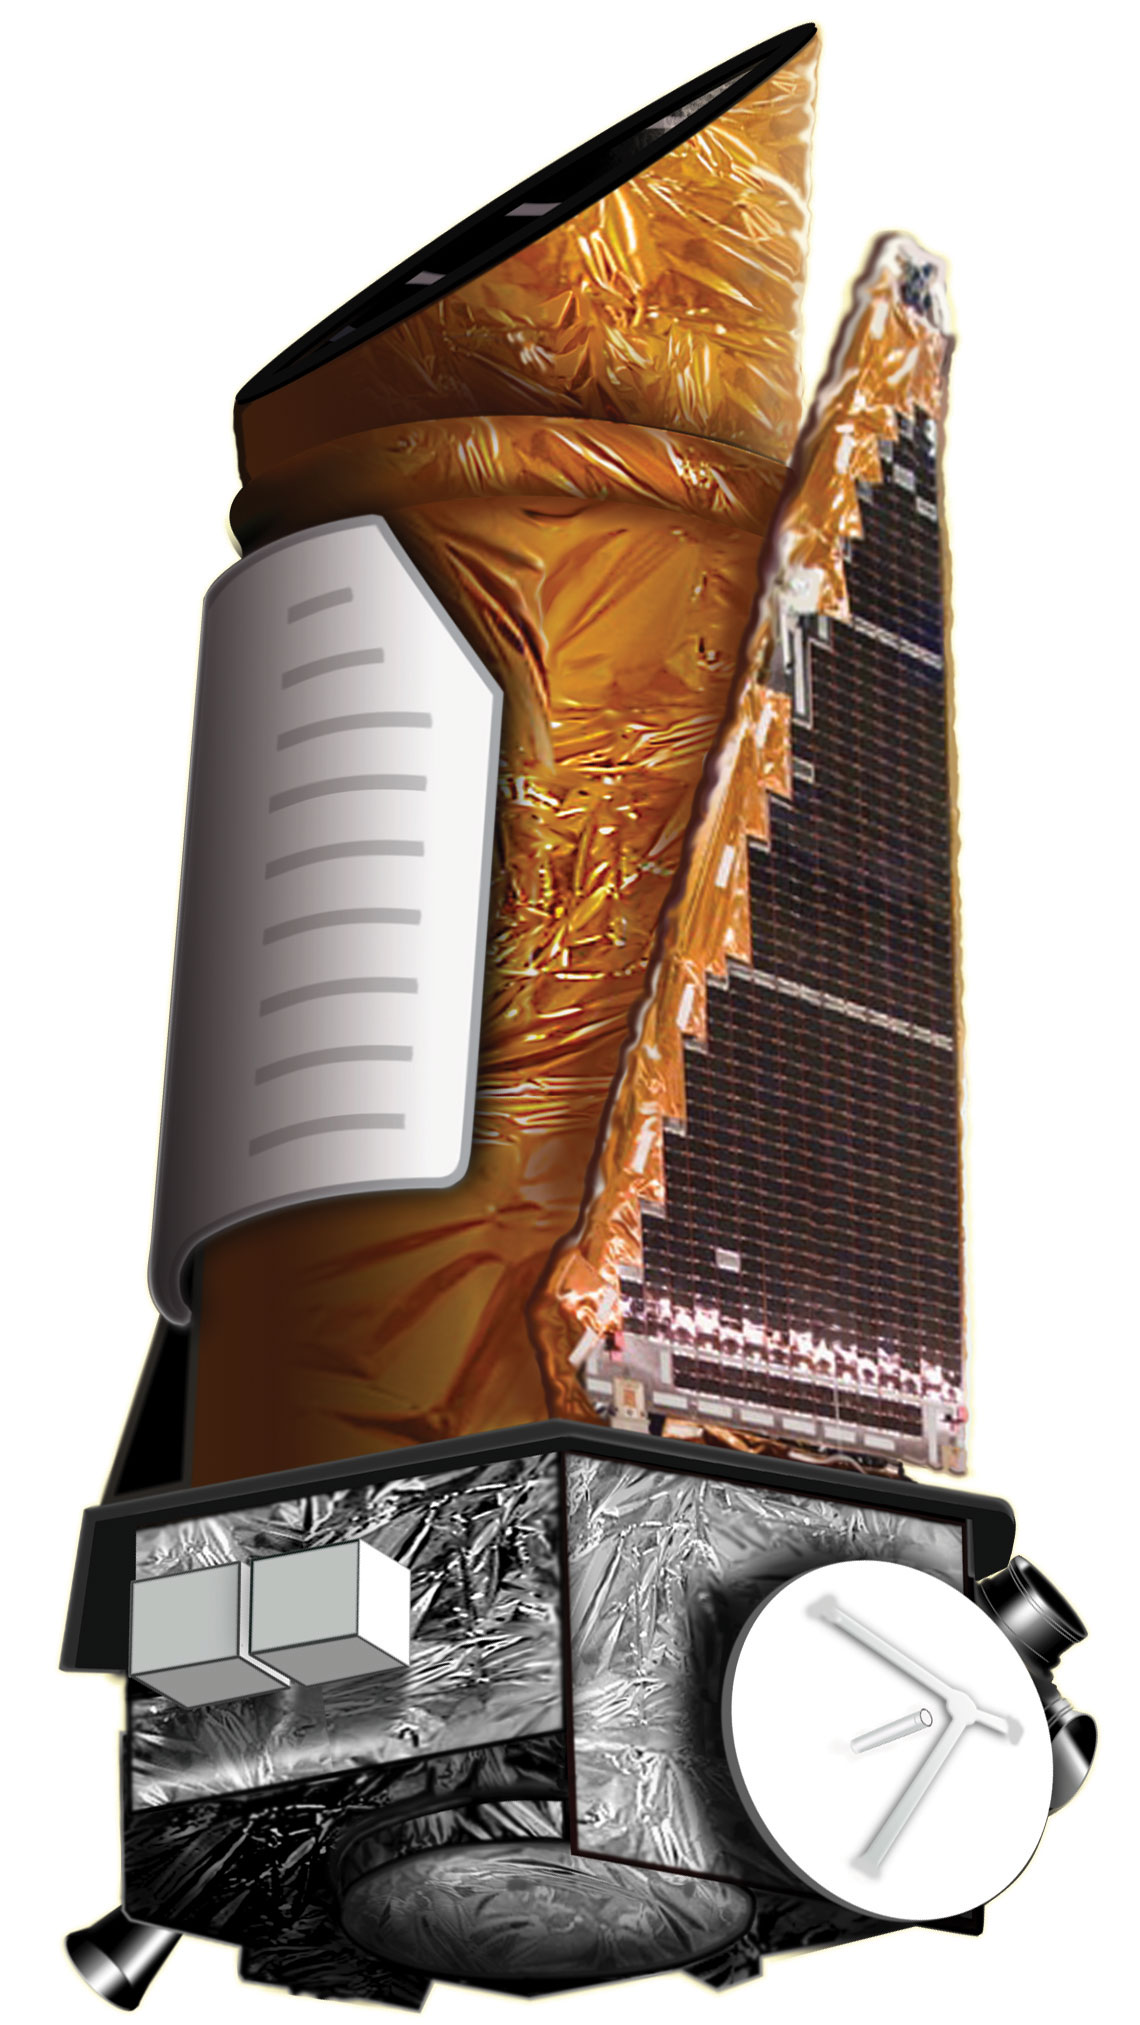
\includegraphics[angle=45,width=1in]{Kepler_spacecraft.png}}
\end{figure*}

\hrule

\vspace{2in}

{\Huge {\bf PA \swversion\ DAWG REVIEW FOR Q0-Q17 LC}}

\vspace{1in}

{\huge Generated \today}
\end{center}


%%%%%%%%%%%%%%%%%%%% CONTENTS SUMMARY SLIDE %%%%%%%%%%%%%%%%%%%%%%%%%

\newcommand{\slideTitle}{{\Huge {\bf PPA \quarter\ LC Data}}}
%
% Copyright 2017 United States Government as represented by the
% Administrator of the National Aeronautics and Space Administration.
% All Rights Reserved.
% 
% This file is available under the terms of the NASA Open Source Agreement
% (NOSA). You should have received a copy of this agreement with the
% Kepler source code; see the file NASA-OPEN-SOURCE-AGREEMENT.doc.
% 
% No Warranty: THE SUBJECT SOFTWARE IS PROVIDED "AS IS" WITHOUT ANY
% WARRANTY OF ANY KIND, EITHER EXPRESSED, IMPLIED, OR STATUTORY,
% INCLUDING, BUT NOT LIMITED TO, ANY WARRANTY THAT THE SUBJECT SOFTWARE
% WILL CONFORM TO SPECIFICATIONS, ANY IMPLIED WARRANTIES OF
% MERCHANTABILITY, FITNESS FOR A PARTICULAR PURPOSE, OR FREEDOM FROM
% INFRINGEMENT, ANY WARRANTY THAT THE SUBJECT SOFTWARE WILL BE ERROR
% FREE, OR ANY WARRANTY THAT DOCUMENTATION, IF PROVIDED, WILL CONFORM
% TO THE SUBJECT SOFTWARE. THIS AGREEMENT DOES NOT, IN ANY MANNER,
% CONSTITUTE AN ENDORSEMENT BY GOVERNMENT AGENCY OR ANY PRIOR RECIPIENT
% OF ANY RESULTS, RESULTING DESIGNS, HARDWARE, SOFTWARE PRODUCTS OR ANY
% OTHER APPLICATIONS RESULTING FROM USE OF THE SUBJECT SOFTWARE.
% FURTHER, GOVERNMENT AGENCY DISCLAIMS ALL WARRANTIES AND LIABILITIES
% REGARDING THIRD-PARTY SOFTWARE, IF PRESENT IN THE ORIGINAL SOFTWARE,
% AND DISTRIBUTES IT "AS IS."
%
% Waiver and Indemnity: RECIPIENT AGREES TO WAIVE ANY AND ALL CLAIMS
% AGAINST THE UNITED STATES GOVERNMENT, ITS CONTRACTORS AND
% SUBCONTRACTORS, AS WELL AS ANY PRIOR RECIPIENT. IF RECIPIENT'S USE OF
% THE SUBJECT SOFTWARE RESULTS IN ANY LIABILITIES, DEMANDS, DAMAGES,
% EXPENSES OR LOSSES ARISING FROM SUCH USE, INCLUDING ANY DAMAGES FROM
% PRODUCTS BASED ON, OR RESULTING FROM, RECIPIENT'S USE OF THE SUBJECT
% SOFTWARE, RECIPIENT SHALL INDEMNIFY AND HOLD HARMLESS THE UNITED
% STATES GOVERNMENT, ITS CONTRACTORS AND SUBCONTRACTORS, AS WELL AS ANY
% PRIOR RECIPIENT, TO THE EXTENT PERMITTED BY LAW. RECIPIENT'S SOLE
% REMEDY FOR ANY SUCH MATTER SHALL BE THE IMMEDIATE, UNILATERAL
% TERMINATION OF THIS AGREEMENT.
%
\cleardoublepage
\begin{figure*}[h!]
  \centering
  \subfigure{\includegraphics[width=1in]{\logo}}
  \hfill
  \slideTitle
  \hfill
  \subfigure{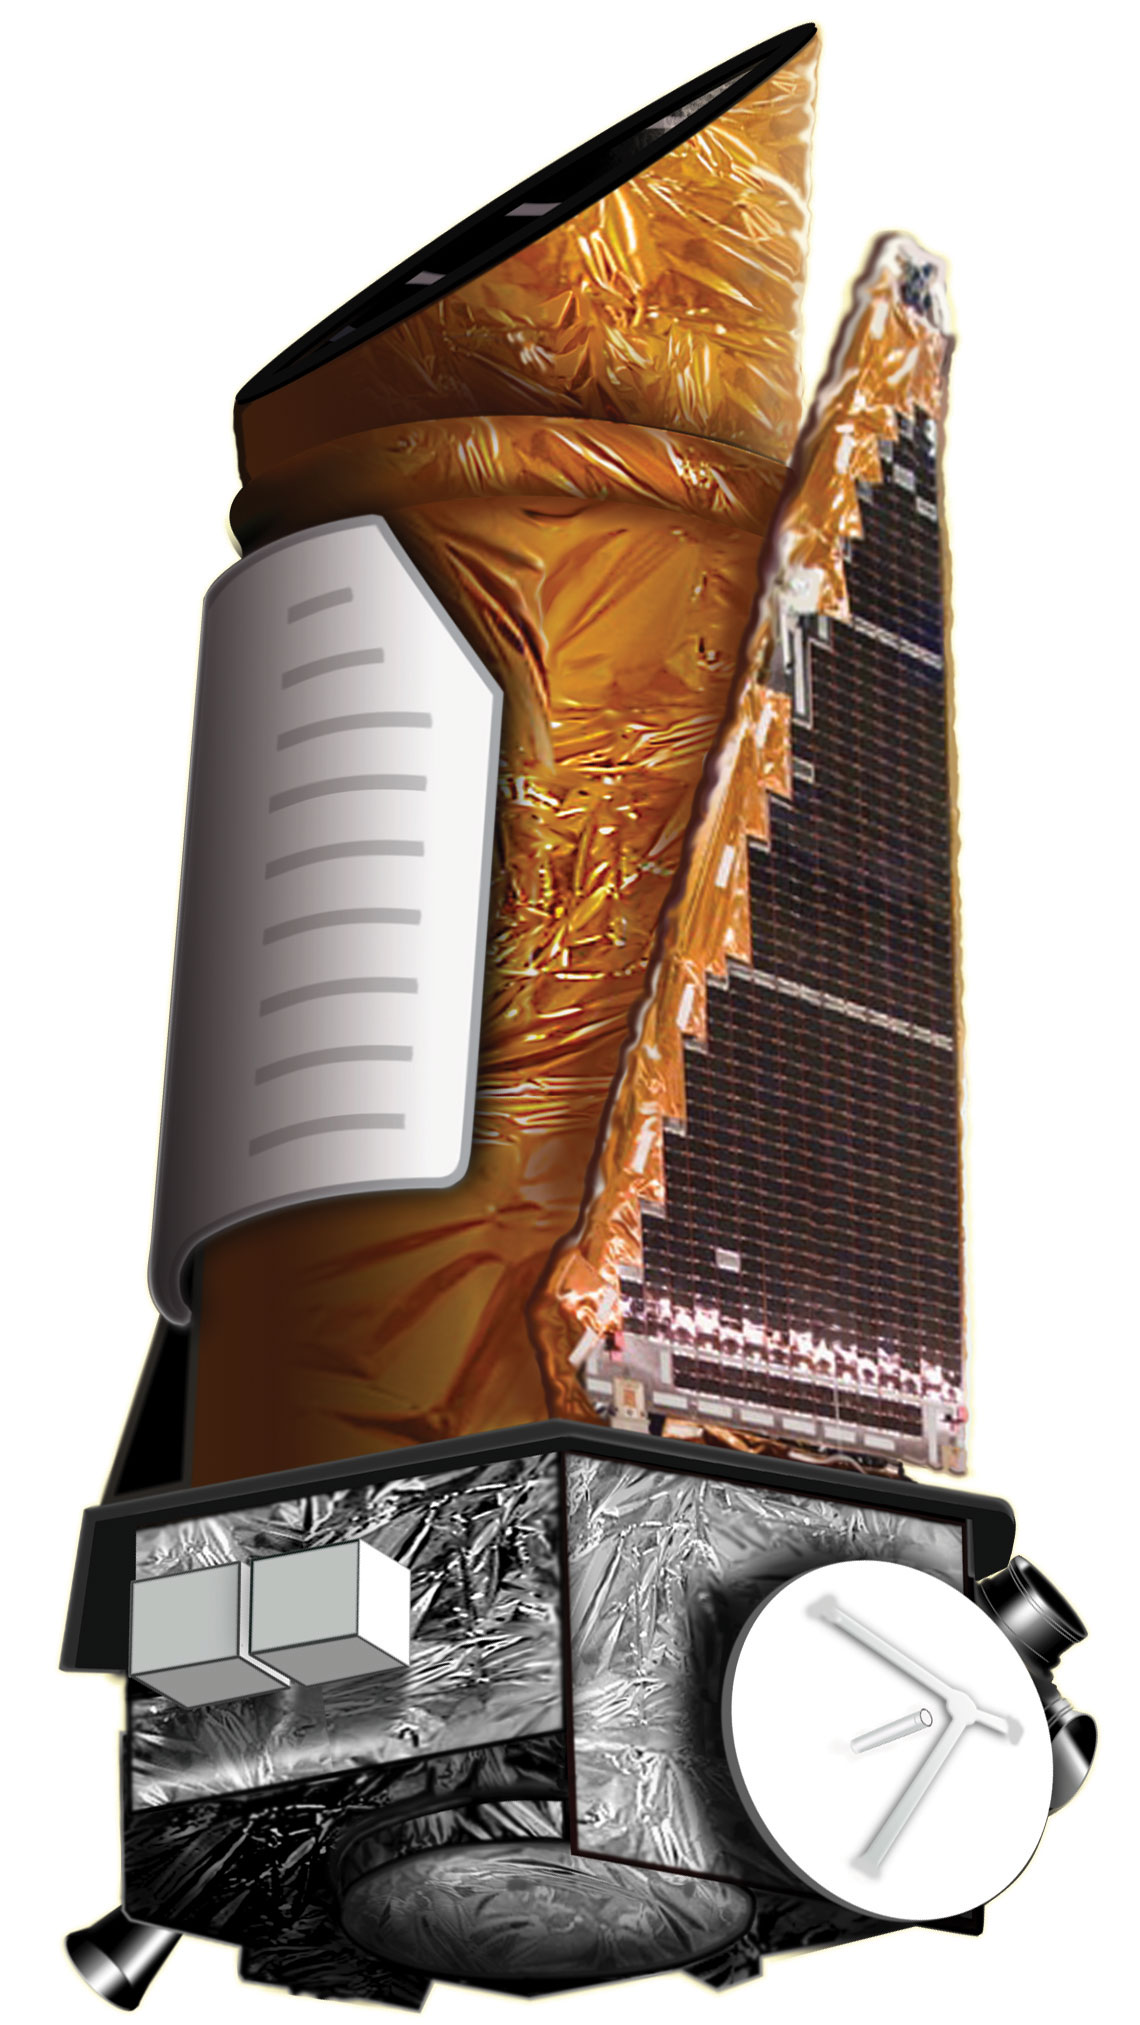
\includegraphics[angle=45,width=1in]{Kepler_spacecraft.png}}
\end{figure*}
\hrule

% Slide for the DAWG presentation intro
% 
% Copyright 2017 United States Government as represented by the
% Administrator of the National Aeronautics and Space Administration.
% All Rights Reserved.
% 
% This file is available under the terms of the NASA Open Source Agreement
% (NOSA). You should have received a copy of this agreement with the
% Kepler source code; see the file NASA-OPEN-SOURCE-AGREEMENT.doc.
% 
% No Warranty: THE SUBJECT SOFTWARE IS PROVIDED "AS IS" WITHOUT ANY
% WARRANTY OF ANY KIND, EITHER EXPRESSED, IMPLIED, OR STATUTORY,
% INCLUDING, BUT NOT LIMITED TO, ANY WARRANTY THAT THE SUBJECT SOFTWARE
% WILL CONFORM TO SPECIFICATIONS, ANY IMPLIED WARRANTIES OF
% MERCHANTABILITY, FITNESS FOR A PARTICULAR PURPOSE, OR FREEDOM FROM
% INFRINGEMENT, ANY WARRANTY THAT THE SUBJECT SOFTWARE WILL BE ERROR
% FREE, OR ANY WARRANTY THAT DOCUMENTATION, IF PROVIDED, WILL CONFORM
% TO THE SUBJECT SOFTWARE. THIS AGREEMENT DOES NOT, IN ANY MANNER,
% CONSTITUTE AN ENDORSEMENT BY GOVERNMENT AGENCY OR ANY PRIOR RECIPIENT
% OF ANY RESULTS, RESULTING DESIGNS, HARDWARE, SOFTWARE PRODUCTS OR ANY
% OTHER APPLICATIONS RESULTING FROM USE OF THE SUBJECT SOFTWARE.
% FURTHER, GOVERNMENT AGENCY DISCLAIMS ALL WARRANTIES AND LIABILITIES
% REGARDING THIRD-PARTY SOFTWARE, IF PRESENT IN THE ORIGINAL SOFTWARE,
% AND DISTRIBUTES IT "AS IS."
%
% Waiver and Indemnity: RECIPIENT AGREES TO WAIVE ANY AND ALL CLAIMS
% AGAINST THE UNITED STATES GOVERNMENT, ITS CONTRACTORS AND
% SUBCONTRACTORS, AS WELL AS ANY PRIOR RECIPIENT. IF RECIPIENT'S USE OF
% THE SUBJECT SOFTWARE RESULTS IN ANY LIABILITIES, DEMANDS, DAMAGES,
% EXPENSES OR LOSSES ARISING FROM SUCH USE, INCLUDING ANY DAMAGES FROM
% PRODUCTS BASED ON, OR RESULTING FROM, RECIPIENT'S USE OF THE SUBJECT
% SOFTWARE, RECIPIENT SHALL INDEMNIFY AND HOLD HARMLESS THE UNITED
% STATES GOVERNMENT, ITS CONTRACTORS AND SUBCONTRACTORS, AS WELL AS ANY
% PRIOR RECIPIENT, TO THE EXTENT PERMITTED BY LAW. RECIPIENT'S SOLE
% REMEDY FOR ANY SUCH MATTER SHALL BE THE IMMEDIATE, UNILATERAL
% TERMINATION OF THIS AGREEMENT.
%
\begin{itemize}

\item Examine long cadence CSCI outputs

  \begin{itemize}
    \item Background polynomial fits
    \item Motion polynomial fits
    \item Raw flux time series including PA-COA metrics
    \item Centroid time series
    \item Detected Cosmic Ray Distribution
    \item Argabrightenings and Reaction wheel zero crossings
  \end{itemize}

%\item Examine short cadence CSCI outputs
%
%  \begin{itemize}
%    \item Raw flux time series
%    \item Centroid time series
%  \end{itemize}

\end{itemize}


%%%%%%%%%%%%%%%%% START THE LC SET OF SLIDES %%%%%%%%%%%%%%%%%%%%%%%%


% attitude comparison
% 
% Copyright 2017 United States Government as represented by the
% Administrator of the National Aeronautics and Space Administration.
% All Rights Reserved.
% 
% NASA acknowledges the SETI Institute's primary role in authoring and
% producing the Kepler Data Processing Pipeline under Cooperative
% Agreement Nos. NNA04CC63A, NNX07AD96A, NNX07AD98A, NNX11AI13A,
% NNX11AI14A, NNX13AD01A & NNX13AD16A.
% 
% This file is available under the terms of the NASA Open Source Agreement
% (NOSA). You should have received a copy of this agreement with the
% Kepler source code; see the file NASA-OPEN-SOURCE-AGREEMENT.doc.
% 
% No Warranty: THE SUBJECT SOFTWARE IS PROVIDED "AS IS" WITHOUT ANY
% WARRANTY OF ANY KIND, EITHER EXPRESSED, IMPLIED, OR STATUTORY,
% INCLUDING, BUT NOT LIMITED TO, ANY WARRANTY THAT THE SUBJECT SOFTWARE
% WILL CONFORM TO SPECIFICATIONS, ANY IMPLIED WARRANTIES OF
% MERCHANTABILITY, FITNESS FOR A PARTICULAR PURPOSE, OR FREEDOM FROM
% INFRINGEMENT, ANY WARRANTY THAT THE SUBJECT SOFTWARE WILL BE ERROR
% FREE, OR ANY WARRANTY THAT DOCUMENTATION, IF PROVIDED, WILL CONFORM
% TO THE SUBJECT SOFTWARE. THIS AGREEMENT DOES NOT, IN ANY MANNER,
% CONSTITUTE AN ENDORSEMENT BY GOVERNMENT AGENCY OR ANY PRIOR RECIPIENT
% OF ANY RESULTS, RESULTING DESIGNS, HARDWARE, SOFTWARE PRODUCTS OR ANY
% OTHER APPLICATIONS RESULTING FROM USE OF THE SUBJECT SOFTWARE.
% FURTHER, GOVERNMENT AGENCY DISCLAIMS ALL WARRANTIES AND LIABILITIES
% REGARDING THIRD-PARTY SOFTWARE, IF PRESENT IN THE ORIGINAL SOFTWARE,
% AND DISTRIBUTES IT "AS IS."
% 
% Waiver and Indemnity: RECIPIENT AGREES TO WAIVE ANY AND ALL CLAIMS
% AGAINST THE UNITED STATES GOVERNMENT, ITS CONTRACTORS AND
% SUBCONTRACTORS, AS WELL AS ANY PRIOR RECIPIENT. IF RECIPIENT'S USE OF
% THE SUBJECT SOFTWARE RESULTS IN ANY LIABILITIES, DEMANDS, DAMAGES,
% EXPENSES OR LOSSES ARISING FROM SUCH USE, INCLUDING ANY DAMAGES FROM
% PRODUCTS BASED ON, OR RESULTING FROM, RECIPIENT'S USE OF THE SUBJECT
% SOFTWARE, RECIPIENT SHALL INDEMNIFY AND HOLD HARMLESS THE UNITED
% STATES GOVERNMENT, ITS CONTRACTORS AND SUBCONTRACTORS, AS WELL AS ANY
% PRIOR RECIPIENT, TO THE EXTENT PERMITTED BY LAW. RECIPIENT'S SOLE
% REMEDY FOR ANY SUCH MATTER SHALL BE THE IMMEDIATE, UNILATERAL
% TERMINATION OF THIS AGREEMENT.
%
\newcommand{\RaAttitudePlot}{\reportgraphicspath pad_pdq_attitude_ra.png}
\newcommand{\DecAttitudePlot}{\reportgraphicspath pad_pdq_attitude_dec.png}
\newcommand{\RollAttitudePlot}{\reportgraphicspath pad_pdq_attitude_roll.png}
\newcommand{\MarAttitudePlot}{\reportgraphicspath pad_pdq_attitude_mar.png}

% focal plane metrics
\newcommand{\BlackPlot}{\reportgraphicspath blackLevel.png}
\newcommand{\BackgroundPlot}{\reportgraphicspath backgroundLevel.png}
\newcommand{\BrightnessPlot}{\reportgraphicspath brightness.png}

\newcommand{\EncircledEnergyPlot}{\reportgraphicspath encircledEnergy.png}
\newcommand{\PlateScalePlot}{\reportgraphicspath plateScale.png}

% pointing metrics
\newcommand{\RowCentroidPlot}{\reportgraphicspath centroidsMeanRow.png}
\newcommand{\ColCentroidPlot}{\reportgraphicspath centroidsMeanColumn.png}

% cdpp metrics 9th, 12th, 15th; 6 hour
\newcommand{\cdppExpectedNinePlot}{\reportgraphicspath cdppExpected_mag9_sixHour.png}
\newcommand{\cdppMeasuredNinePlot}{\reportgraphicspath cdppMeasured_mag9_sixHour.png}
\newcommand{\cdppRatioNinePlot}{\reportgraphicspath cdppRatio_mag9_sixHour.png}
\newcommand{\cdppExpectedTwelvePlot}{\reportgraphicspath cdppExpected_mag12_sixHour.png}
\newcommand{\cdppMeasuredTwelvePlot}{\reportgraphicspath cdppMeasured_mag12_sixHour.png}
\newcommand{\cdppRatioTwelvePlot}{\reportgraphicspath cdppRatio_mag12_sixHour.png}
\newcommand{\cdppExpectedFifteenPlot}{\reportgraphicspath cdppExpected_mag15_sixHour.png}
\newcommand{\cdppMeasuredFifteenPlot}{\reportgraphicspath cdppMeasured_mag15_sixHour.png}
\newcommand{\cdppRatioFifteenPlot}{\reportgraphicspath cdppRatio_mag15_sixHour.png}

% seasonal CDPP comparision plots
\newcommand{\deltaCdppNinePlot}{\reportgraphicspath delta_cdpp_6hr_9mag.png}
\newcommand{\deltaCdppTwelvePlot}{\reportgraphicspath delta_cdpp_6hr_12mag.png}
\newcommand{\deltaCdppFourteenPlot}{\reportgraphicspath delta_cdpp_6hr_14mag.png}
\newcommand{\cdppCompChanNinePlot}{\reportgraphicspath cdpp_channel_6hr_9mag.png}
\newcommand{\cdppCompChanTwelvePlot}{\reportgraphicspath cdpp_channel_6hr_12mag.png}
\newcommand{\cdppCompChanFourteenPlot}{\reportgraphicspath cdpp_channel_6hr_14mag.png}

% compression metrics
%%%% need to fix these so that they don't have to be edited for each run!
\newcommand{\TheoreticalCompressionPlot}{\reportgraphicspath pag_theoretical_compression_efficiency.png}
\newcommand{\AchievedCompressionPlot}{\reportgraphicspath pag_achieved_compression_efficiency.png}
\newcommand{\TheoreticalCompressionChannelPlot}{\reportgraphicspath theoreticalCompressionEfficiency.png}
\newcommand{\AchievedCompressionChannelPlot}{\reportgraphicspath achievedCompressionEfficiency.png}
\newcommand{\TheoreticalCompressionChannelPlotZoom}{\reportgraphicspath theoreticalCompressionEfficiencyZoom.png}
\newcommand{\AchievedCompressionChannelPlotZoom}{\reportgraphicspath achievedCompressionEfficiencyZoom.png}

%%START SLIDE 
% 
% Copyright 2017 United States Government as represented by the
% Administrator of the National Aeronautics and Space Administration.
% All Rights Reserved.
% 
% NASA acknowledges the SETI Institute's primary role in authoring and
% producing the Kepler Data Processing Pipeline under Cooperative
% Agreement Nos. NNA04CC63A, NNX07AD96A, NNX07AD98A, NNX11AI13A,
% NNX11AI14A, NNX13AD01A & NNX13AD16A.
% 
% This file is available under the terms of the NASA Open Source Agreement
% (NOSA). You should have received a copy of this agreement with the
% Kepler source code; see the file NASA-OPEN-SOURCE-AGREEMENT.doc.
% 
% No Warranty: THE SUBJECT SOFTWARE IS PROVIDED "AS IS" WITHOUT ANY
% WARRANTY OF ANY KIND, EITHER EXPRESSED, IMPLIED, OR STATUTORY,
% INCLUDING, BUT NOT LIMITED TO, ANY WARRANTY THAT THE SUBJECT SOFTWARE
% WILL CONFORM TO SPECIFICATIONS, ANY IMPLIED WARRANTIES OF
% MERCHANTABILITY, FITNESS FOR A PARTICULAR PURPOSE, OR FREEDOM FROM
% INFRINGEMENT, ANY WARRANTY THAT THE SUBJECT SOFTWARE WILL BE ERROR
% FREE, OR ANY WARRANTY THAT DOCUMENTATION, IF PROVIDED, WILL CONFORM
% TO THE SUBJECT SOFTWARE. THIS AGREEMENT DOES NOT, IN ANY MANNER,
% CONSTITUTE AN ENDORSEMENT BY GOVERNMENT AGENCY OR ANY PRIOR RECIPIENT
% OF ANY RESULTS, RESULTING DESIGNS, HARDWARE, SOFTWARE PRODUCTS OR ANY
% OTHER APPLICATIONS RESULTING FROM USE OF THE SUBJECT SOFTWARE.
% FURTHER, GOVERNMENT AGENCY DISCLAIMS ALL WARRANTIES AND LIABILITIES
% REGARDING THIRD-PARTY SOFTWARE, IF PRESENT IN THE ORIGINAL SOFTWARE,
% AND DISTRIBUTES IT "AS IS."
% 
% Waiver and Indemnity: RECIPIENT AGREES TO WAIVE ANY AND ALL CLAIMS
% AGAINST THE UNITED STATES GOVERNMENT, ITS CONTRACTORS AND
% SUBCONTRACTORS, AS WELL AS ANY PRIOR RECIPIENT. IF RECIPIENT'S USE OF
% THE SUBJECT SOFTWARE RESULTS IN ANY LIABILITIES, DEMANDS, DAMAGES,
% EXPENSES OR LOSSES ARISING FROM SUCH USE, INCLUDING ANY DAMAGES FROM
% PRODUCTS BASED ON, OR RESULTING FROM, RECIPIENT'S USE OF THE SUBJECT
% SOFTWARE, RECIPIENT SHALL INDEMNIFY AND HOLD HARMLESS THE UNITED
% STATES GOVERNMENT, ITS CONTRACTORS AND SUBCONTRACTORS, AS WELL AS ANY
% PRIOR RECIPIENT, TO THE EXTENT PERMITTED BY LAW. RECIPIENT'S SOLE
% REMEDY FOR ANY SUCH MATTER SHALL BE THE IMMEDIATE, UNILATERAL
% TERMINATION OF THIS AGREEMENT.
%
\cleardoublepage
\begin{figure*}[h!]
  \centering
  \subfigure{\includegraphics[width=1in]{\logo}}
  \hfill
  {\Huge {\bf \quarter\ PAD/PDQ Attitude Comparison}}
  \hfill
  \subfigure{\includegraphics[angle=90,width=1.0in]{\spacecraft}}
\end{figure*}
\hrule
\begin{figure*}[h!]
  \centering
  \subfigure{\includegraphics[height=0.37\textheight]{\RaAttitudePlot}}
  \subfigure{\includegraphics[height=0.37\textheight]{\DecAttitudePlot}}
  \hfill
  \subfigure{\includegraphics[height=0.37\textheight]{\RollAttitudePlot}}
  \caption{PA/PDQ RA, Dec, Roll comparison}
\end{figure*}
%% END SLIDE 

%%START SLIDE 
\cleardoublepage
\begin{figure*}[h!]
  \centering
  \subfigure{\includegraphics[width=1in]{\logo}}
  \hfill
  {\Huge {\bf \quarter\ PAD/PDQ Attitude Comparison}}
  \hfill
  \subfigure{\includegraphics[angle=90,width=1in]{\spacecraft}}
\end{figure*}
\hrule
\begin{figure*}[h!]
  \centering
  \includegraphics[width=0.7\textwidth]{\MarAttitudePlot}
  \caption{LC Smear and Dark Levels (e-/exposure)}
\end{figure*}
%% END SLIDE 

%%START SLIDE 
\cleardoublepage
\begin{figure*}[h!]
  \centering
  \subfigure{\includegraphics[width=1in]{\logo}}
  \hfill
  {\Huge {\bf \quarter\ PAD Row and Column Centroid}}
  \hfill
  \subfigure{\includegraphics[angle=90,width=1.0in]{\spacecraft}}
\end{figure*}
\hrule
\begin{figure*}[h!]
  \centering
  \subfigure{\includegraphics[width=0.47\textwidth]{\RowCentroidPlot}}
  \subfigure{\includegraphics[width=0.47\textwidth]{\ColCentroidPlot}}
  \caption{Row and Column centroids for \quarter.}
\end{figure*}
%% END SLIDE 

%%START SLIDE 
% 
% Copyright 2017 United States Government as represented by the
% Administrator of the National Aeronautics and Space Administration.
% All Rights Reserved.
% 
% NASA acknowledges the SETI Institute's primary role in authoring and
% producing the Kepler Data Processing Pipeline under Cooperative
% Agreement Nos. NNA04CC63A, NNX07AD96A, NNX07AD98A, NNX11AI13A,
% NNX11AI14A, NNX13AD01A & NNX13AD16A.
% 
% This file is available under the terms of the NASA Open Source Agreement
% (NOSA). You should have received a copy of this agreement with the
% Kepler source code; see the file NASA-OPEN-SOURCE-AGREEMENT.doc.
% 
% No Warranty: THE SUBJECT SOFTWARE IS PROVIDED "AS IS" WITHOUT ANY
% WARRANTY OF ANY KIND, EITHER EXPRESSED, IMPLIED, OR STATUTORY,
% INCLUDING, BUT NOT LIMITED TO, ANY WARRANTY THAT THE SUBJECT SOFTWARE
% WILL CONFORM TO SPECIFICATIONS, ANY IMPLIED WARRANTIES OF
% MERCHANTABILITY, FITNESS FOR A PARTICULAR PURPOSE, OR FREEDOM FROM
% INFRINGEMENT, ANY WARRANTY THAT THE SUBJECT SOFTWARE WILL BE ERROR
% FREE, OR ANY WARRANTY THAT DOCUMENTATION, IF PROVIDED, WILL CONFORM
% TO THE SUBJECT SOFTWARE. THIS AGREEMENT DOES NOT, IN ANY MANNER,
% CONSTITUTE AN ENDORSEMENT BY GOVERNMENT AGENCY OR ANY PRIOR RECIPIENT
% OF ANY RESULTS, RESULTING DESIGNS, HARDWARE, SOFTWARE PRODUCTS OR ANY
% OTHER APPLICATIONS RESULTING FROM USE OF THE SUBJECT SOFTWARE.
% FURTHER, GOVERNMENT AGENCY DISCLAIMS ALL WARRANTIES AND LIABILITIES
% REGARDING THIRD-PARTY SOFTWARE, IF PRESENT IN THE ORIGINAL SOFTWARE,
% AND DISTRIBUTES IT "AS IS."
% 
% Waiver and Indemnity: RECIPIENT AGREES TO WAIVE ANY AND ALL CLAIMS
% AGAINST THE UNITED STATES GOVERNMENT, ITS CONTRACTORS AND
% SUBCONTRACTORS, AS WELL AS ANY PRIOR RECIPIENT. IF RECIPIENT'S USE OF
% THE SUBJECT SOFTWARE RESULTS IN ANY LIABILITIES, DEMANDS, DAMAGES,
% EXPENSES OR LOSSES ARISING FROM SUCH USE, INCLUDING ANY DAMAGES FROM
% PRODUCTS BASED ON, OR RESULTING FROM, RECIPIENT'S USE OF THE SUBJECT
% SOFTWARE, RECIPIENT SHALL INDEMNIFY AND HOLD HARMLESS THE UNITED
% STATES GOVERNMENT, ITS CONTRACTORS AND SUBCONTRACTORS, AS WELL AS ANY
% PRIOR RECIPIENT, TO THE EXTENT PERMITTED BY LAW. RECIPIENT'S SOLE
% REMEDY FOR ANY SUCH MATTER SHALL BE THE IMMEDIATE, UNILATERAL
% TERMINATION OF THIS AGREEMENT.
%
\cleardoublepage
\begin{figure*}[h!]
  \centering
  \subfigure{\includegraphics[width=1in]{\logo}}
  \hfill
  {\Huge {\bf \quarter\ PAD Black Level}}
  \hfill
  \subfigure{\includegraphics[angle=90,width=1.0in]{\spacecraft}}
\end{figure*}
\hrule
\begin{figure*}[h!]
  \centering
  \includegraphics[height=0.755555\textheight]{\BlackPlot}
  \caption{Black Level}
\end{figure*}
%% END SLIDE 

%%START SLIDE 
\cleardoublepage
\begin{figure*}[h!]
  \centering
  \subfigure{\includegraphics[width=1in]{\logo}}
  \hfill
  {\Huge {\bf \quarter\ PAD Background and Brightness}}
  \hfill
  \subfigure{\includegraphics[angle=90,width=1.0in]{\spacecraft}}
\end{figure*}
\hrule
\begin{figure*}[h!]
  \centering
  \subfigure{\includegraphics[width=0.47\textwidth]{\BackgroundPlot}}
  \subfigure{\includegraphics[width=0.47\textwidth]{\BrightnessPlot}}
  \caption{PAD Background and Brightness metric}
\end{figure*}
%% END SLIDE 

%%START SLIDE 
\cleardoublepage
\begin{figure*}[h!]
  \centering
  \subfigure{\includegraphics[width=1in]{\logo}}
  \hfill
  {\Huge {\bf \quarter\ PAD Encircled Energy and Platescale}}
  \hfill
  \subfigure{\includegraphics[angle=90,width=1.0in]{\spacecraft}}
\end{figure*}
\hrule
\begin{figure*}[h!]
  \centering
  \subfigure{\includegraphics[width=0.47\textwidth]{\EncircledEnergyPlot}}
  \subfigure{\includegraphics[width=0.47\textwidth]{\PlateScalePlot}}
  \caption{PAD Encircled Energy and Platescale}
\end{figure*}
%% END SLIDE 

%%START SLIDE 
% 
% Copyright 2017 United States Government as represented by the
% Administrator of the National Aeronautics and Space Administration.
% All Rights Reserved.
% 
% NASA acknowledges the SETI Institute's primary role in authoring and
% producing the Kepler Data Processing Pipeline under Cooperative
% Agreement Nos. NNA04CC63A, NNX07AD96A, NNX07AD98A, NNX11AI13A,
% NNX11AI14A, NNX13AD01A & NNX13AD16A.
% 
% This file is available under the terms of the NASA Open Source Agreement
% (NOSA). You should have received a copy of this agreement with the
% Kepler source code; see the file NASA-OPEN-SOURCE-AGREEMENT.doc.
% 
% No Warranty: THE SUBJECT SOFTWARE IS PROVIDED "AS IS" WITHOUT ANY
% WARRANTY OF ANY KIND, EITHER EXPRESSED, IMPLIED, OR STATUTORY,
% INCLUDING, BUT NOT LIMITED TO, ANY WARRANTY THAT THE SUBJECT SOFTWARE
% WILL CONFORM TO SPECIFICATIONS, ANY IMPLIED WARRANTIES OF
% MERCHANTABILITY, FITNESS FOR A PARTICULAR PURPOSE, OR FREEDOM FROM
% INFRINGEMENT, ANY WARRANTY THAT THE SUBJECT SOFTWARE WILL BE ERROR
% FREE, OR ANY WARRANTY THAT DOCUMENTATION, IF PROVIDED, WILL CONFORM
% TO THE SUBJECT SOFTWARE. THIS AGREEMENT DOES NOT, IN ANY MANNER,
% CONSTITUTE AN ENDORSEMENT BY GOVERNMENT AGENCY OR ANY PRIOR RECIPIENT
% OF ANY RESULTS, RESULTING DESIGNS, HARDWARE, SOFTWARE PRODUCTS OR ANY
% OTHER APPLICATIONS RESULTING FROM USE OF THE SUBJECT SOFTWARE.
% FURTHER, GOVERNMENT AGENCY DISCLAIMS ALL WARRANTIES AND LIABILITIES
% REGARDING THIRD-PARTY SOFTWARE, IF PRESENT IN THE ORIGINAL SOFTWARE,
% AND DISTRIBUTES IT "AS IS."
% 
% Waiver and Indemnity: RECIPIENT AGREES TO WAIVE ANY AND ALL CLAIMS
% AGAINST THE UNITED STATES GOVERNMENT, ITS CONTRACTORS AND
% SUBCONTRACTORS, AS WELL AS ANY PRIOR RECIPIENT. IF RECIPIENT'S USE OF
% THE SUBJECT SOFTWARE RESULTS IN ANY LIABILITIES, DEMANDS, DAMAGES,
% EXPENSES OR LOSSES ARISING FROM SUCH USE, INCLUDING ANY DAMAGES FROM
% PRODUCTS BASED ON, OR RESULTING FROM, RECIPIENT'S USE OF THE SUBJECT
% SOFTWARE, RECIPIENT SHALL INDEMNIFY AND HOLD HARMLESS THE UNITED
% STATES GOVERNMENT, ITS CONTRACTORS AND SUBCONTRACTORS, AS WELL AS ANY
% PRIOR RECIPIENT, TO THE EXTENT PERMITTED BY LAW. RECIPIENT'S SOLE
% REMEDY FOR ANY SUCH MATTER SHALL BE THE IMMEDIATE, UNILATERAL
% TERMINATION OF THIS AGREEMENT.
%
\cleardoublepage
\begin{figure*}[h!]
  \centering
  \subfigure{\includegraphics[width=1in]{\logo}}
  \hfill
  {\Huge {\bf \quarter\ PAD CDPP: $9^{th}$ mag, 6 hr}}
  \hfill
  \subfigure{\includegraphics[angle=90,width=1.0in]{\spacecraft}}
\end{figure*}
\hrule
\begin{figure*}[h!]
  \centering
  \subfigure{\includegraphics[height=0.37\textheight]{\cdppExpectedNinePlot}}
  \subfigure{\includegraphics[height=0.37\textheight]{\cdppMeasuredNinePlot}}
  \hfill
  \subfigure{\includegraphics[height=0.37\textheight]{\cdppRatioNinePlot}}
  \caption{$9^{th}$ mag 6 hr CDPP}
\end{figure*}
%% END SLIDE 

%%START SLIDE 
\cleardoublepage
\begin{figure*}[h!]
  \centering
  \subfigure{\includegraphics[width=1in]{\logo}}
  \hfill
  {\Huge {\bf \quarter\ PAD CDPP: $12^{th}$ mag, 6 hr}}
  \hfill
  \subfigure{\includegraphics[angle=90,width=1.0in]{\spacecraft}}
\end{figure*}
\hrule
\begin{figure*}[h!]
  \centering
  \subfigure{\includegraphics[height=0.37\textheight]{\cdppExpectedTwelvePlot}}
  \subfigure{\includegraphics[height=0.37\textheight]{\cdppMeasuredTwelvePlot}}
  \hfill
  \subfigure{\includegraphics[height=0.37\textheight]{\cdppRatioTwelvePlot}}
  \caption{$12^{th}$ mag 6 hr CDPP}
\end{figure*}
%% END SLIDE 

%%START SLIDE 
\cleardoublepage
\begin{figure*}[h!]
  \centering
  \subfigure{\includegraphics[width=1in]{\logo}}
  \hfill
  {\Huge {\bf \quarter\ PAD CDPP: $15^{th}$ mag, 6 hr}}
  \hfill
  \subfigure{\includegraphics[angle=90,width=1.0in]{\spacecraft}}
\end{figure*}
\hrule
\begin{figure*}[h!]
  \centering
  \subfigure{\includegraphics[height=0.37\textheight]{\cdppExpectedFifteenPlot}}
  \subfigure{\includegraphics[height=0.37\textheight]{\cdppMeasuredFifteenPlot}}
  \hfill
  \subfigure{\includegraphics[height=0.37\textheight]{\cdppRatioFifteenPlot}}
  \caption{$15^{th}$ mag 6 hr CDPP}
\end{figure*}
%% END SLIDE 

% optional cdpp plots, TURN OFF if cdpp_seasonal_comparison_plotter.m was not run
%%%START SLIDE  -focal plane plot
% 
% Copyright 2017 United States Government as represented by the
% Administrator of the National Aeronautics and Space Administration.
% All Rights Reserved.
% 
% NASA acknowledges the SETI Institute's primary role in authoring and
% producing the Kepler Data Processing Pipeline under Cooperative
% Agreement Nos. NNA04CC63A, NNX07AD96A, NNX07AD98A, NNX11AI13A,
% NNX11AI14A, NNX13AD01A & NNX13AD16A.
% 
% This file is available under the terms of the NASA Open Source Agreement
% (NOSA). You should have received a copy of this agreement with the
% Kepler source code; see the file NASA-OPEN-SOURCE-AGREEMENT.doc.
% 
% No Warranty: THE SUBJECT SOFTWARE IS PROVIDED "AS IS" WITHOUT ANY
% WARRANTY OF ANY KIND, EITHER EXPRESSED, IMPLIED, OR STATUTORY,
% INCLUDING, BUT NOT LIMITED TO, ANY WARRANTY THAT THE SUBJECT SOFTWARE
% WILL CONFORM TO SPECIFICATIONS, ANY IMPLIED WARRANTIES OF
% MERCHANTABILITY, FITNESS FOR A PARTICULAR PURPOSE, OR FREEDOM FROM
% INFRINGEMENT, ANY WARRANTY THAT THE SUBJECT SOFTWARE WILL BE ERROR
% FREE, OR ANY WARRANTY THAT DOCUMENTATION, IF PROVIDED, WILL CONFORM
% TO THE SUBJECT SOFTWARE. THIS AGREEMENT DOES NOT, IN ANY MANNER,
% CONSTITUTE AN ENDORSEMENT BY GOVERNMENT AGENCY OR ANY PRIOR RECIPIENT
% OF ANY RESULTS, RESULTING DESIGNS, HARDWARE, SOFTWARE PRODUCTS OR ANY
% OTHER APPLICATIONS RESULTING FROM USE OF THE SUBJECT SOFTWARE.
% FURTHER, GOVERNMENT AGENCY DISCLAIMS ALL WARRANTIES AND LIABILITIES
% REGARDING THIRD-PARTY SOFTWARE, IF PRESENT IN THE ORIGINAL SOFTWARE,
% AND DISTRIBUTES IT "AS IS."
% 
% Waiver and Indemnity: RECIPIENT AGREES TO WAIVE ANY AND ALL CLAIMS
% AGAINST THE UNITED STATES GOVERNMENT, ITS CONTRACTORS AND
% SUBCONTRACTORS, AS WELL AS ANY PRIOR RECIPIENT. IF RECIPIENT'S USE OF
% THE SUBJECT SOFTWARE RESULTS IN ANY LIABILITIES, DEMANDS, DAMAGES,
% EXPENSES OR LOSSES ARISING FROM SUCH USE, INCLUDING ANY DAMAGES FROM
% PRODUCTS BASED ON, OR RESULTING FROM, RECIPIENT'S USE OF THE SUBJECT
% SOFTWARE, RECIPIENT SHALL INDEMNIFY AND HOLD HARMLESS THE UNITED
% STATES GOVERNMENT, ITS CONTRACTORS AND SUBCONTRACTORS, AS WELL AS ANY
% PRIOR RECIPIENT, TO THE EXTENT PERMITTED BY LAW. RECIPIENT'S SOLE
% REMEDY FOR ANY SUCH MATTER SHALL BE THE IMMEDIATE, UNILATERAL
% TERMINATION OF THIS AGREEMENT.
%
\cleardoublepage
\begin{figure*}[h!]
  \centering
  \subfigure{\includegraphics[width=1in]{\logo}}
  \hfill
  {\Huge {\bf \quarter\ PAD CDPP: Seasonal Comparision }}
  \hfill
  \subfigure{\includegraphics[angle=90,width=1.0in]{\spacecraft}}
\end{figure*}
\hrule
\begin{figure*}[h!]
  \centering
  \subfigure{\includegraphics[height=0.37\textheight]{\deltaCdppNinePlot}}
  \subfigure{\includegraphics[height=0.37\textheight]{\deltaCdppTwelvePlot}}
  \hfill
  \subfigure{\includegraphics[height=0.37\textheight]{\deltaCdppFourteenPlot}}
  \caption{$9^{th}$, $12^{th}$, $14^{th}$ mag 6 hr Seasonal CDPP comparison}
\end{figure*}
%% END SLIDE 

%%START SLIDE  - line plot
\cleardoublepage
\begin{figure*}[h!]
  \centering
  \subfigure{\includegraphics[width=1in]{\logo}}
  \hfill
  {\Huge {\bf \quarter\ PAD CDPP: Seasonal Comparision }}
  \hfill
  \subfigure{\includegraphics[angle=90,width=1.0in]{\spacecraft}}
\end{figure*}
\hrule
\begin{figure*}[h!]
  \centering
  \subfigure{\includegraphics[height=0.37\textheight]{\cdppCompChanNinePlot}}
  \subfigure{\includegraphics[height=0.37\textheight]{\cdppCompChanTwelvePlot}}
  \hfill
  \subfigure{\includegraphics[height=0.37\textheight]{\cdppCompChanFourteenPlot}}
  \caption{$9^{th}$, $12^{th}$, $14^{th}$ mag 6 hr Seasonal CDPP comparison}
\end{figure*}
%% END SLIDE 

%%START SLIDE 
%\cleardoublepage
%\begin{figure*}[h!]
%  \centering
%  \subfigure{\includegraphics[width=1in]{\logo}}
%  \hfill
%  {\Huge {\bf \quarter\ PAD CDPP: $12^{th}$ mag, 6 hr}}
%  \hfill
%  \subfigure{\includegraphics[angle=90,width=1.0in]{\spacecraft}}
%\end{figure*}
%\hrule
%\begin{figure*}[h!]
%  \centering
%  \subfigure{\includegraphics[height=0.37\textheight]{\cdppExpectedTwelvePlot}}
%  \subfigure{\includegraphics[height=0.37\textheight]{\cdppMeasuredTwelvePlot}}
%  \hfill
%  \subfigure{\includegraphics[height=0.37\textheight]{\cdppRatioTwelvePlot}}
%  \caption{$12^{th}$ mag 6 hr CDPP}
%\end{figure*}
%% END SLIDE 

%%START SLIDE 
%\cleardoublepage
%\begin{figure*}[h!]
%  \centering
%  \subfigure{\includegraphics[width=1in]{\logo}}
%  \hfill
%  {\Huge {\bf \quarter\ PAD CDPP: $15^{th}$ mag, 6 hr}}
%  \hfill
%  \subfigure{\includegraphics[angle=90,width=1.0in]{\spacecraft}}
%\end{figure*}
%\hrule
%\begin{figure*}[h!]
%  \centering
%  \subfigure{\includegraphics[height=0.37\textheight]{\cdppExpectedFifteenPlot}}
%  \subfigure{\includegraphics[height=0.37\textheight]{\cdppMeasuredFifteenPlot}}
%  \hfill
%  \subfigure{\includegraphics[height=0.37\textheight]{\cdppRatioFifteenPlot}}
%  \caption{$15^{th}$ mag 6 hr CDPP}
%\end{figure*}
%% END SLIDE 


%%START SLIDE 
% 
% Copyright 2017 United States Government as represented by the
% Administrator of the National Aeronautics and Space Administration.
% All Rights Reserved.
% 
% NASA acknowledges the SETI Institute's primary role in authoring and
% producing the Kepler Data Processing Pipeline under Cooperative
% Agreement Nos. NNA04CC63A, NNX07AD96A, NNX07AD98A, NNX11AI13A,
% NNX11AI14A, NNX13AD01A & NNX13AD16A.
% 
% This file is available under the terms of the NASA Open Source Agreement
% (NOSA). You should have received a copy of this agreement with the
% Kepler source code; see the file NASA-OPEN-SOURCE-AGREEMENT.doc.
% 
% No Warranty: THE SUBJECT SOFTWARE IS PROVIDED "AS IS" WITHOUT ANY
% WARRANTY OF ANY KIND, EITHER EXPRESSED, IMPLIED, OR STATUTORY,
% INCLUDING, BUT NOT LIMITED TO, ANY WARRANTY THAT THE SUBJECT SOFTWARE
% WILL CONFORM TO SPECIFICATIONS, ANY IMPLIED WARRANTIES OF
% MERCHANTABILITY, FITNESS FOR A PARTICULAR PURPOSE, OR FREEDOM FROM
% INFRINGEMENT, ANY WARRANTY THAT THE SUBJECT SOFTWARE WILL BE ERROR
% FREE, OR ANY WARRANTY THAT DOCUMENTATION, IF PROVIDED, WILL CONFORM
% TO THE SUBJECT SOFTWARE. THIS AGREEMENT DOES NOT, IN ANY MANNER,
% CONSTITUTE AN ENDORSEMENT BY GOVERNMENT AGENCY OR ANY PRIOR RECIPIENT
% OF ANY RESULTS, RESULTING DESIGNS, HARDWARE, SOFTWARE PRODUCTS OR ANY
% OTHER APPLICATIONS RESULTING FROM USE OF THE SUBJECT SOFTWARE.
% FURTHER, GOVERNMENT AGENCY DISCLAIMS ALL WARRANTIES AND LIABILITIES
% REGARDING THIRD-PARTY SOFTWARE, IF PRESENT IN THE ORIGINAL SOFTWARE,
% AND DISTRIBUTES IT "AS IS."
% 
% Waiver and Indemnity: RECIPIENT AGREES TO WAIVE ANY AND ALL CLAIMS
% AGAINST THE UNITED STATES GOVERNMENT, ITS CONTRACTORS AND
% SUBCONTRACTORS, AS WELL AS ANY PRIOR RECIPIENT. IF RECIPIENT'S USE OF
% THE SUBJECT SOFTWARE RESULTS IN ANY LIABILITIES, DEMANDS, DAMAGES,
% EXPENSES OR LOSSES ARISING FROM SUCH USE, INCLUDING ANY DAMAGES FROM
% PRODUCTS BASED ON, OR RESULTING FROM, RECIPIENT'S USE OF THE SUBJECT
% SOFTWARE, RECIPIENT SHALL INDEMNIFY AND HOLD HARMLESS THE UNITED
% STATES GOVERNMENT, ITS CONTRACTORS AND SUBCONTRACTORS, AS WELL AS ANY
% PRIOR RECIPIENT, TO THE EXTENT PERMITTED BY LAW. RECIPIENT'S SOLE
% REMEDY FOR ANY SUCH MATTER SHALL BE THE IMMEDIATE, UNILATERAL
% TERMINATION OF THIS AGREEMENT.
%
\cleardoublepage
\begin{figure*}[h!]
  \centering
  \subfigure{\includegraphics[width=1in]{\logo}}
  \hfill
  {\Huge {\bf \quarter\ PAG Compression}}
  \hfill
  \subfigure{\includegraphics[angle=90,width=1.0in]{\spacecraft}}
\end{figure*}
\hrule
\begin{figure*}[h!]
  \centering
  \subfigure{\includegraphics[width=0.47\textwidth]{\TheoreticalCompressionPlot}}
  \subfigure{\includegraphics[width=0.47\textwidth]{\AchievedCompressionPlot}}
  \caption{PAG Theoretical and Achieved compression metrics}
\end{figure*}

\cleardoublepage
\begin{figure*}[h!]
  \centering
  \subfigure{\includegraphics[width=1in]{\logo}}
  \hfill
  {\Huge {\bf \quarter\ PAG Channel-level Compression}}
  \hfill
  \subfigure{\includegraphics[angle=90,width=1.0in]{\spacecraft}}
\end{figure*}
\hrule
\begin{figure*}[h!]
  \centering
  \subfigure{\includegraphics[width=0.47\textwidth]{\TheoreticalCompressionChannelPlot}}
  \subfigure{\includegraphics[width=0.47\textwidth]{\AchievedCompressionChannelPlot}}
  \caption{PAG Theoretical and Achieved compression metrics for each channel}
\end{figure*}

%\cleardoublepage
%\begin{figure*}[h!]
%  \centering
%  \subfigure{\includegraphics[width=1in]{\logo}}
%  \hfill
%  {\Huge {\bf \quarter\ PAG Channel-level Compression - Zoomed}}
%  \hfill
%  \subfigure{\includegraphics[angle=90,width=1.0in]{\spacecraft}}
%\end{figure*}
%\hrule
%\begin{figure*}[h!]
%  \centering
%  \subfigure{\includegraphics[width=0.47\textwidth]{\TheoreticalCompressionChannelPlotZoom}}
%  \subfigure{\includegraphics[width=0.47\textwidth]{\AchievedCompressionChannelPlotZoom}}
%  \caption{PAG Theoretical and Achieved compression metrics for each channel}
%\end{figure*}
%% END SLIDE 


%%%%%%%%%%%%%%%%% START THE SC SET OF SLIDES %%%%%%%%%%%%%%%%%%%%%%%%

%% Start Section title slide
%\cleardoublepage
%\renewcommand{\slideTitle}{{\Huge {\bf \quarter\ SC}}}
%%
% Copyright 2017 United States Government as represented by the
% Administrator of the National Aeronautics and Space Administration.
% All Rights Reserved.
% 
% This file is available under the terms of the NASA Open Source Agreement
% (NOSA). You should have received a copy of this agreement with the
% Kepler source code; see the file NASA-OPEN-SOURCE-AGREEMENT.doc.
% 
% No Warranty: THE SUBJECT SOFTWARE IS PROVIDED "AS IS" WITHOUT ANY
% WARRANTY OF ANY KIND, EITHER EXPRESSED, IMPLIED, OR STATUTORY,
% INCLUDING, BUT NOT LIMITED TO, ANY WARRANTY THAT THE SUBJECT SOFTWARE
% WILL CONFORM TO SPECIFICATIONS, ANY IMPLIED WARRANTIES OF
% MERCHANTABILITY, FITNESS FOR A PARTICULAR PURPOSE, OR FREEDOM FROM
% INFRINGEMENT, ANY WARRANTY THAT THE SUBJECT SOFTWARE WILL BE ERROR
% FREE, OR ANY WARRANTY THAT DOCUMENTATION, IF PROVIDED, WILL CONFORM
% TO THE SUBJECT SOFTWARE. THIS AGREEMENT DOES NOT, IN ANY MANNER,
% CONSTITUTE AN ENDORSEMENT BY GOVERNMENT AGENCY OR ANY PRIOR RECIPIENT
% OF ANY RESULTS, RESULTING DESIGNS, HARDWARE, SOFTWARE PRODUCTS OR ANY
% OTHER APPLICATIONS RESULTING FROM USE OF THE SUBJECT SOFTWARE.
% FURTHER, GOVERNMENT AGENCY DISCLAIMS ALL WARRANTIES AND LIABILITIES
% REGARDING THIRD-PARTY SOFTWARE, IF PRESENT IN THE ORIGINAL SOFTWARE,
% AND DISTRIBUTES IT "AS IS."
%
% Waiver and Indemnity: RECIPIENT AGREES TO WAIVE ANY AND ALL CLAIMS
% AGAINST THE UNITED STATES GOVERNMENT, ITS CONTRACTORS AND
% SUBCONTRACTORS, AS WELL AS ANY PRIOR RECIPIENT. IF RECIPIENT'S USE OF
% THE SUBJECT SOFTWARE RESULTS IN ANY LIABILITIES, DEMANDS, DAMAGES,
% EXPENSES OR LOSSES ARISING FROM SUCH USE, INCLUDING ANY DAMAGES FROM
% PRODUCTS BASED ON, OR RESULTING FROM, RECIPIENT'S USE OF THE SUBJECT
% SOFTWARE, RECIPIENT SHALL INDEMNIFY AND HOLD HARMLESS THE UNITED
% STATES GOVERNMENT, ITS CONTRACTORS AND SUBCONTRACTORS, AS WELL AS ANY
% PRIOR RECIPIENT, TO THE EXTENT PERMITTED BY LAW. RECIPIENT'S SOLE
% REMEDY FOR ANY SUCH MATTER SHALL BE THE IMMEDIATE, UNILATERAL
% TERMINATION OF THIS AGREEMENT.
%
\cleardoublepage
\begin{figure*}[h!]
  \centering
  \subfigure{\includegraphics[width=1in]{\logo}}
  \hfill
  \slideTitle
  \hfill
  \subfigure{\includegraphics[angle=45,width=1in]{Kepler_spacecraft.png}}
\end{figure*}
\hrule

%%% End Section title slide
%
%%
% Copyright 2017 United States Government as represented by the
% Administrator of the National Aeronautics and Space Administration.
% All Rights Reserved.
% 
% NASA acknowledges the SETI Institute's primary role in authoring and
% producing the Kepler Data Processing Pipeline under Cooperative
% Agreement Nos. NNA04CC63A, NNX07AD96A, NNX07AD98A, NNX11AI13A,
% NNX11AI14A, NNX13AD01A & NNX13AD16A.
% 
% This file is available under the terms of the NASA Open Source Agreement
% (NOSA). You should have received a copy of this agreement with the
% Kepler source code; see the file NASA-OPEN-SOURCE-AGREEMENT.doc.
% 
% No Warranty: THE SUBJECT SOFTWARE IS PROVIDED "AS IS" WITHOUT ANY
% WARRANTY OF ANY KIND, EITHER EXPRESSED, IMPLIED, OR STATUTORY,
% INCLUDING, BUT NOT LIMITED TO, ANY WARRANTY THAT THE SUBJECT SOFTWARE
% WILL CONFORM TO SPECIFICATIONS, ANY IMPLIED WARRANTIES OF
% MERCHANTABILITY, FITNESS FOR A PARTICULAR PURPOSE, OR FREEDOM FROM
% INFRINGEMENT, ANY WARRANTY THAT THE SUBJECT SOFTWARE WILL BE ERROR
% FREE, OR ANY WARRANTY THAT DOCUMENTATION, IF PROVIDED, WILL CONFORM
% TO THE SUBJECT SOFTWARE. THIS AGREEMENT DOES NOT, IN ANY MANNER,
% CONSTITUTE AN ENDORSEMENT BY GOVERNMENT AGENCY OR ANY PRIOR RECIPIENT
% OF ANY RESULTS, RESULTING DESIGNS, HARDWARE, SOFTWARE PRODUCTS OR ANY
% OTHER APPLICATIONS RESULTING FROM USE OF THE SUBJECT SOFTWARE.
% FURTHER, GOVERNMENT AGENCY DISCLAIMS ALL WARRANTIES AND LIABILITIES
% REGARDING THIRD-PARTY SOFTWARE, IF PRESENT IN THE ORIGINAL SOFTWARE,
% AND DISTRIBUTES IT "AS IS."
% 
% Waiver and Indemnity: RECIPIENT AGREES TO WAIVE ANY AND ALL CLAIMS
% AGAINST THE UNITED STATES GOVERNMENT, ITS CONTRACTORS AND
% SUBCONTRACTORS, AS WELL AS ANY PRIOR RECIPIENT. IF RECIPIENT'S USE OF
% THE SUBJECT SOFTWARE RESULTS IN ANY LIABILITIES, DEMANDS, DAMAGES,
% EXPENSES OR LOSSES ARISING FROM SUCH USE, INCLUDING ANY DAMAGES FROM
% PRODUCTS BASED ON, OR RESULTING FROM, RECIPIENT'S USE OF THE SUBJECT
% SOFTWARE, RECIPIENT SHALL INDEMNIFY AND HOLD HARMLESS THE UNITED
% STATES GOVERNMENT, ITS CONTRACTORS AND SUBCONTRACTORS, AS WELL AS ANY
% PRIOR RECIPIENT, TO THE EXTENT PERMITTED BY LAW. RECIPIENT'S SOLE
% REMEDY FOR ANY SUCH MATTER SHALL BE THE IMMEDIATE, UNILATERAL
% TERMINATION OF THIS AGREEMENT.
%
\renewcommand{\channel}{19}
\renewcommand{\channelCharacteristics}{Nominal}
\renewcommand{\BlackResidualsImage}{\scPipelineFigsMOne pipeline_figures_ch19/cal_black_residuals_imagesc.png}
\renewcommand{\BlackResidualsPlot}{\scPipelineFigsMOne pipeline_figures_ch19/cal_black_residuals_plot.png}
\renewcommand{\BestBlackPolyOrder}{\scPipelineFigsMOne pipeline_figures_ch19/cal_black_correction_over_pixels_plot.png}
\renewcommand{\BlackResidualsMesh}{\scPipelineFigsMOne pipeline_figures_ch19/cal_black_residuals_mesh.png}
\renewcommand{\SmearDifferenceImage}{\scPipelineFigsMOne pipeline_figures_ch19/cal_smear_difference_imagesc.png}
\renewcommand{\SmearDifferencePlot}{\scPipelineFigsMOne pipeline_figures_ch19/cal_smear_difference_plot.png}
\renewcommand{\SmearDifferenceMesh}{\scPipelineFigsMOne pipeline_figures_ch19/cal_smear_difference_mesh.png}
\renewcommand{\SmearAndDarkLevelsPlot}{\scPipelineFigsMOne pipeline_figures_ch19/cal_smear_and_dark_levels_plot.png}

\newcommand{\PhotometricPixelsInVsOutUOne}{\scPhotometricFigsMOne photometric_figures_m1_ch19/sc_ch19_uow1_in_vs_out.png}
\newcommand{\PhotometricPixelsInVsOutRatioUOne}{\scPhotometricFigsMOne photometric_figures_m1_ch19/sc_ch19_uow1_in_vs_outinratio.png}

\newcommand{\PhotometricPixelsInVsOutUTwo}{\scPhotometricFigsMOne photometric_figures_m1_ch19/sc_ch19_uow2_in_vs_out.png}
\newcommand{\PhotometricPixelsInVsOutRatioUTwo}{\scPhotometricFigsMOne photometric_figures_m1_ch19/sc_ch19_uow2_in_vs_outinratio.png}

\newcommand{\PhotometricPixelsInVsOutUThree}{\scPhotometricFigsMOne photometric_figures_m1_ch19/sc_ch19_uow3_in_vs_out.png}
\newcommand{\PhotometricPixelsInVsOutRatioUThree}{\scPhotometricFigsMOne photometric_figures_m1_ch19/sc_ch19_uow3_in_vs_outinratio.png}

%%%START SLIDE 
% 
% Copyright 2017 United States Government as represented by the
% Administrator of the National Aeronautics and Space Administration.
% All Rights Reserved.
% 
% NASA acknowledges the SETI Institute's primary role in authoring and
% producing the Kepler Data Processing Pipeline under Cooperative
% Agreement Nos. NNA04CC63A, NNX07AD96A, NNX07AD98A, NNX11AI13A,
% NNX11AI14A, NNX13AD01A & NNX13AD16A.
% 
% This file is available under the terms of the NASA Open Source Agreement
% (NOSA). You should have received a copy of this agreement with the
% Kepler source code; see the file NASA-OPEN-SOURCE-AGREEMENT.doc.
% 
% No Warranty: THE SUBJECT SOFTWARE IS PROVIDED "AS IS" WITHOUT ANY
% WARRANTY OF ANY KIND, EITHER EXPRESSED, IMPLIED, OR STATUTORY,
% INCLUDING, BUT NOT LIMITED TO, ANY WARRANTY THAT THE SUBJECT SOFTWARE
% WILL CONFORM TO SPECIFICATIONS, ANY IMPLIED WARRANTIES OF
% MERCHANTABILITY, FITNESS FOR A PARTICULAR PURPOSE, OR FREEDOM FROM
% INFRINGEMENT, ANY WARRANTY THAT THE SUBJECT SOFTWARE WILL BE ERROR
% FREE, OR ANY WARRANTY THAT DOCUMENTATION, IF PROVIDED, WILL CONFORM
% TO THE SUBJECT SOFTWARE. THIS AGREEMENT DOES NOT, IN ANY MANNER,
% CONSTITUTE AN ENDORSEMENT BY GOVERNMENT AGENCY OR ANY PRIOR RECIPIENT
% OF ANY RESULTS, RESULTING DESIGNS, HARDWARE, SOFTWARE PRODUCTS OR ANY
% OTHER APPLICATIONS RESULTING FROM USE OF THE SUBJECT SOFTWARE.
% FURTHER, GOVERNMENT AGENCY DISCLAIMS ALL WARRANTIES AND LIABILITIES
% REGARDING THIRD-PARTY SOFTWARE, IF PRESENT IN THE ORIGINAL SOFTWARE,
% AND DISTRIBUTES IT "AS IS."
% 
% Waiver and Indemnity: RECIPIENT AGREES TO WAIVE ANY AND ALL CLAIMS
% AGAINST THE UNITED STATES GOVERNMENT, ITS CONTRACTORS AND
% SUBCONTRACTORS, AS WELL AS ANY PRIOR RECIPIENT. IF RECIPIENT'S USE OF
% THE SUBJECT SOFTWARE RESULTS IN ANY LIABILITIES, DEMANDS, DAMAGES,
% EXPENSES OR LOSSES ARISING FROM SUCH USE, INCLUDING ANY DAMAGES FROM
% PRODUCTS BASED ON, OR RESULTING FROM, RECIPIENT'S USE OF THE SUBJECT
% SOFTWARE, RECIPIENT SHALL INDEMNIFY AND HOLD HARMLESS THE UNITED
% STATES GOVERNMENT, ITS CONTRACTORS AND SUBCONTRACTORS, AS WELL AS ANY
% PRIOR RECIPIENT, TO THE EXTENT PERMITTED BY LAW. RECIPIENT'S SOLE
% REMEDY FOR ANY SUCH MATTER SHALL BE THE IMMEDIATE, UNILATERAL
% TERMINATION OF THIS AGREEMENT.
%
\cleardoublepage

\renewcommand{\slideTitle}{{\Huge {\bf SC Channel \channel\ \channelCharacteristics}}}
%
% Copyright 2017 United States Government as represented by the
% Administrator of the National Aeronautics and Space Administration.
% All Rights Reserved.
% 
% This file is available under the terms of the NASA Open Source Agreement
% (NOSA). You should have received a copy of this agreement with the
% Kepler source code; see the file NASA-OPEN-SOURCE-AGREEMENT.doc.
% 
% No Warranty: THE SUBJECT SOFTWARE IS PROVIDED "AS IS" WITHOUT ANY
% WARRANTY OF ANY KIND, EITHER EXPRESSED, IMPLIED, OR STATUTORY,
% INCLUDING, BUT NOT LIMITED TO, ANY WARRANTY THAT THE SUBJECT SOFTWARE
% WILL CONFORM TO SPECIFICATIONS, ANY IMPLIED WARRANTIES OF
% MERCHANTABILITY, FITNESS FOR A PARTICULAR PURPOSE, OR FREEDOM FROM
% INFRINGEMENT, ANY WARRANTY THAT THE SUBJECT SOFTWARE WILL BE ERROR
% FREE, OR ANY WARRANTY THAT DOCUMENTATION, IF PROVIDED, WILL CONFORM
% TO THE SUBJECT SOFTWARE. THIS AGREEMENT DOES NOT, IN ANY MANNER,
% CONSTITUTE AN ENDORSEMENT BY GOVERNMENT AGENCY OR ANY PRIOR RECIPIENT
% OF ANY RESULTS, RESULTING DESIGNS, HARDWARE, SOFTWARE PRODUCTS OR ANY
% OTHER APPLICATIONS RESULTING FROM USE OF THE SUBJECT SOFTWARE.
% FURTHER, GOVERNMENT AGENCY DISCLAIMS ALL WARRANTIES AND LIABILITIES
% REGARDING THIRD-PARTY SOFTWARE, IF PRESENT IN THE ORIGINAL SOFTWARE,
% AND DISTRIBUTES IT "AS IS."
%
% Waiver and Indemnity: RECIPIENT AGREES TO WAIVE ANY AND ALL CLAIMS
% AGAINST THE UNITED STATES GOVERNMENT, ITS CONTRACTORS AND
% SUBCONTRACTORS, AS WELL AS ANY PRIOR RECIPIENT. IF RECIPIENT'S USE OF
% THE SUBJECT SOFTWARE RESULTS IN ANY LIABILITIES, DEMANDS, DAMAGES,
% EXPENSES OR LOSSES ARISING FROM SUCH USE, INCLUDING ANY DAMAGES FROM
% PRODUCTS BASED ON, OR RESULTING FROM, RECIPIENT'S USE OF THE SUBJECT
% SOFTWARE, RECIPIENT SHALL INDEMNIFY AND HOLD HARMLESS THE UNITED
% STATES GOVERNMENT, ITS CONTRACTORS AND SUBCONTRACTORS, AS WELL AS ANY
% PRIOR RECIPIENT, TO THE EXTENT PERMITTED BY LAW. RECIPIENT'S SOLE
% REMEDY FOR ANY SUCH MATTER SHALL BE THE IMMEDIATE, UNILATERAL
% TERMINATION OF THIS AGREEMENT.
%
\cleardoublepage
\begin{figure*}[h!]
  \centering
  \subfigure{\includegraphics[width=1in]{\logo}}
  \hfill
  \slideTitle
  \hfill
  \subfigure{\includegraphics[angle=45,width=1in]{Kepler_spacecraft.png}}
\end{figure*}
\hrule


%% END SLIDE 

%%START SLIDE 
\cleardoublepage

\renewcommand{\slideTitle}{{\Huge {\bf \quarter\ SC Channel \channel\ black residuals}}}
%
% Copyright 2017 United States Government as represented by the
% Administrator of the National Aeronautics and Space Administration.
% All Rights Reserved.
% 
% This file is available under the terms of the NASA Open Source Agreement
% (NOSA). You should have received a copy of this agreement with the
% Kepler source code; see the file NASA-OPEN-SOURCE-AGREEMENT.doc.
% 
% No Warranty: THE SUBJECT SOFTWARE IS PROVIDED "AS IS" WITHOUT ANY
% WARRANTY OF ANY KIND, EITHER EXPRESSED, IMPLIED, OR STATUTORY,
% INCLUDING, BUT NOT LIMITED TO, ANY WARRANTY THAT THE SUBJECT SOFTWARE
% WILL CONFORM TO SPECIFICATIONS, ANY IMPLIED WARRANTIES OF
% MERCHANTABILITY, FITNESS FOR A PARTICULAR PURPOSE, OR FREEDOM FROM
% INFRINGEMENT, ANY WARRANTY THAT THE SUBJECT SOFTWARE WILL BE ERROR
% FREE, OR ANY WARRANTY THAT DOCUMENTATION, IF PROVIDED, WILL CONFORM
% TO THE SUBJECT SOFTWARE. THIS AGREEMENT DOES NOT, IN ANY MANNER,
% CONSTITUTE AN ENDORSEMENT BY GOVERNMENT AGENCY OR ANY PRIOR RECIPIENT
% OF ANY RESULTS, RESULTING DESIGNS, HARDWARE, SOFTWARE PRODUCTS OR ANY
% OTHER APPLICATIONS RESULTING FROM USE OF THE SUBJECT SOFTWARE.
% FURTHER, GOVERNMENT AGENCY DISCLAIMS ALL WARRANTIES AND LIABILITIES
% REGARDING THIRD-PARTY SOFTWARE, IF PRESENT IN THE ORIGINAL SOFTWARE,
% AND DISTRIBUTES IT "AS IS."
%
% Waiver and Indemnity: RECIPIENT AGREES TO WAIVE ANY AND ALL CLAIMS
% AGAINST THE UNITED STATES GOVERNMENT, ITS CONTRACTORS AND
% SUBCONTRACTORS, AS WELL AS ANY PRIOR RECIPIENT. IF RECIPIENT'S USE OF
% THE SUBJECT SOFTWARE RESULTS IN ANY LIABILITIES, DEMANDS, DAMAGES,
% EXPENSES OR LOSSES ARISING FROM SUCH USE, INCLUDING ANY DAMAGES FROM
% PRODUCTS BASED ON, OR RESULTING FROM, RECIPIENT'S USE OF THE SUBJECT
% SOFTWARE, RECIPIENT SHALL INDEMNIFY AND HOLD HARMLESS THE UNITED
% STATES GOVERNMENT, ITS CONTRACTORS AND SUBCONTRACTORS, AS WELL AS ANY
% PRIOR RECIPIENT, TO THE EXTENT PERMITTED BY LAW. RECIPIENT'S SOLE
% REMEDY FOR ANY SUCH MATTER SHALL BE THE IMMEDIATE, UNILATERAL
% TERMINATION OF THIS AGREEMENT.
%
\cleardoublepage
\begin{figure*}[h!]
  \centering
  \subfigure{\includegraphics[width=1in]{\logo}}
  \hfill
  \slideTitle
  \hfill
  \subfigure{\includegraphics[angle=45,width=1in]{Kepler_spacecraft.png}}
\end{figure*}
\hrule


\begin{figure*}[h!]
  \centering
  \subfigure{\includegraphics[width=0.5\textwidth]{\BlackResidualsImage}}
  \subfigure{\includegraphics[width=0.45\textwidth]{\BlackResidualsPlot}}
  \subfigure{\includegraphics[width=5in,height=1.8in]{\BestBlackPolyOrder}}
  \subfigure{\includegraphics[height=1.8in]{\BlackResidualsMesh}}
  \caption{LC Black Residuals (ADU/exposure) for Channel \channel}
  \subfigure{\includegraphics[width=4in]{\lcBlackResidualsImageChannel19}}
  \subfigure{\includegraphics[width=2in]{\lcBlackResidualsPlotChannel19}}
%  \subfigure{\includegraphics[width=4in]{\lcBlackResidualsImageChannel39}}
%  \subfigure{\includegraphics[width=2in]{\lcBlackResidualsPlotChannel39}}
\end{figure*}
%% END SLIDE 

%%START SLIDE 
\cleardoublepage

\renewcommand{\slideTitle}{{\Huge {\bf \quarter\ SC Channel \channel\ smear residuals}}}
%
% Copyright 2017 United States Government as represented by the
% Administrator of the National Aeronautics and Space Administration.
% All Rights Reserved.
% 
% This file is available under the terms of the NASA Open Source Agreement
% (NOSA). You should have received a copy of this agreement with the
% Kepler source code; see the file NASA-OPEN-SOURCE-AGREEMENT.doc.
% 
% No Warranty: THE SUBJECT SOFTWARE IS PROVIDED "AS IS" WITHOUT ANY
% WARRANTY OF ANY KIND, EITHER EXPRESSED, IMPLIED, OR STATUTORY,
% INCLUDING, BUT NOT LIMITED TO, ANY WARRANTY THAT THE SUBJECT SOFTWARE
% WILL CONFORM TO SPECIFICATIONS, ANY IMPLIED WARRANTIES OF
% MERCHANTABILITY, FITNESS FOR A PARTICULAR PURPOSE, OR FREEDOM FROM
% INFRINGEMENT, ANY WARRANTY THAT THE SUBJECT SOFTWARE WILL BE ERROR
% FREE, OR ANY WARRANTY THAT DOCUMENTATION, IF PROVIDED, WILL CONFORM
% TO THE SUBJECT SOFTWARE. THIS AGREEMENT DOES NOT, IN ANY MANNER,
% CONSTITUTE AN ENDORSEMENT BY GOVERNMENT AGENCY OR ANY PRIOR RECIPIENT
% OF ANY RESULTS, RESULTING DESIGNS, HARDWARE, SOFTWARE PRODUCTS OR ANY
% OTHER APPLICATIONS RESULTING FROM USE OF THE SUBJECT SOFTWARE.
% FURTHER, GOVERNMENT AGENCY DISCLAIMS ALL WARRANTIES AND LIABILITIES
% REGARDING THIRD-PARTY SOFTWARE, IF PRESENT IN THE ORIGINAL SOFTWARE,
% AND DISTRIBUTES IT "AS IS."
%
% Waiver and Indemnity: RECIPIENT AGREES TO WAIVE ANY AND ALL CLAIMS
% AGAINST THE UNITED STATES GOVERNMENT, ITS CONTRACTORS AND
% SUBCONTRACTORS, AS WELL AS ANY PRIOR RECIPIENT. IF RECIPIENT'S USE OF
% THE SUBJECT SOFTWARE RESULTS IN ANY LIABILITIES, DEMANDS, DAMAGES,
% EXPENSES OR LOSSES ARISING FROM SUCH USE, INCLUDING ANY DAMAGES FROM
% PRODUCTS BASED ON, OR RESULTING FROM, RECIPIENT'S USE OF THE SUBJECT
% SOFTWARE, RECIPIENT SHALL INDEMNIFY AND HOLD HARMLESS THE UNITED
% STATES GOVERNMENT, ITS CONTRACTORS AND SUBCONTRACTORS, AS WELL AS ANY
% PRIOR RECIPIENT, TO THE EXTENT PERMITTED BY LAW. RECIPIENT'S SOLE
% REMEDY FOR ANY SUCH MATTER SHALL BE THE IMMEDIATE, UNILATERAL
% TERMINATION OF THIS AGREEMENT.
%
\cleardoublepage
\begin{figure*}[h!]
  \centering
  \subfigure{\includegraphics[width=1in]{\logo}}
  \hfill
  \slideTitle
  \hfill
  \subfigure{\includegraphics[angle=45,width=1in]{Kepler_spacecraft.png}}
\end{figure*}
\hrule


\begin{figure*}[h!]
  \centering
  \subfigure{\includegraphics[width=0.43\textwidth]{\SmearDifferenceImage}}
  \subfigure{\includegraphics[width=0.43\textwidth]{\SmearDifferencePlot}}
  \hfill
  \subfigure{\includegraphics[width=0.25\textwidth]{\SmearDifferenceMesh}}
  \caption{LC Smear Residuals (ADU/exposure) for Channel \channel}
\end{figure*}
%% END SLIDE 

%%START SLIDE 
\cleardoublepage

\renewcommand{\slideTitle}{{\Huge {\bf \quarter\ SC Channel \channel\ smear and dark levels}}}
%
% Copyright 2017 United States Government as represented by the
% Administrator of the National Aeronautics and Space Administration.
% All Rights Reserved.
% 
% This file is available under the terms of the NASA Open Source Agreement
% (NOSA). You should have received a copy of this agreement with the
% Kepler source code; see the file NASA-OPEN-SOURCE-AGREEMENT.doc.
% 
% No Warranty: THE SUBJECT SOFTWARE IS PROVIDED "AS IS" WITHOUT ANY
% WARRANTY OF ANY KIND, EITHER EXPRESSED, IMPLIED, OR STATUTORY,
% INCLUDING, BUT NOT LIMITED TO, ANY WARRANTY THAT THE SUBJECT SOFTWARE
% WILL CONFORM TO SPECIFICATIONS, ANY IMPLIED WARRANTIES OF
% MERCHANTABILITY, FITNESS FOR A PARTICULAR PURPOSE, OR FREEDOM FROM
% INFRINGEMENT, ANY WARRANTY THAT THE SUBJECT SOFTWARE WILL BE ERROR
% FREE, OR ANY WARRANTY THAT DOCUMENTATION, IF PROVIDED, WILL CONFORM
% TO THE SUBJECT SOFTWARE. THIS AGREEMENT DOES NOT, IN ANY MANNER,
% CONSTITUTE AN ENDORSEMENT BY GOVERNMENT AGENCY OR ANY PRIOR RECIPIENT
% OF ANY RESULTS, RESULTING DESIGNS, HARDWARE, SOFTWARE PRODUCTS OR ANY
% OTHER APPLICATIONS RESULTING FROM USE OF THE SUBJECT SOFTWARE.
% FURTHER, GOVERNMENT AGENCY DISCLAIMS ALL WARRANTIES AND LIABILITIES
% REGARDING THIRD-PARTY SOFTWARE, IF PRESENT IN THE ORIGINAL SOFTWARE,
% AND DISTRIBUTES IT "AS IS."
%
% Waiver and Indemnity: RECIPIENT AGREES TO WAIVE ANY AND ALL CLAIMS
% AGAINST THE UNITED STATES GOVERNMENT, ITS CONTRACTORS AND
% SUBCONTRACTORS, AS WELL AS ANY PRIOR RECIPIENT. IF RECIPIENT'S USE OF
% THE SUBJECT SOFTWARE RESULTS IN ANY LIABILITIES, DEMANDS, DAMAGES,
% EXPENSES OR LOSSES ARISING FROM SUCH USE, INCLUDING ANY DAMAGES FROM
% PRODUCTS BASED ON, OR RESULTING FROM, RECIPIENT'S USE OF THE SUBJECT
% SOFTWARE, RECIPIENT SHALL INDEMNIFY AND HOLD HARMLESS THE UNITED
% STATES GOVERNMENT, ITS CONTRACTORS AND SUBCONTRACTORS, AS WELL AS ANY
% PRIOR RECIPIENT, TO THE EXTENT PERMITTED BY LAW. RECIPIENT'S SOLE
% REMEDY FOR ANY SUCH MATTER SHALL BE THE IMMEDIATE, UNILATERAL
% TERMINATION OF THIS AGREEMENT.
%
\cleardoublepage
\begin{figure*}[h!]
  \centering
  \subfigure{\includegraphics[width=1in]{\logo}}
  \hfill
  \slideTitle
  \hfill
  \subfigure{\includegraphics[angle=45,width=1in]{Kepler_spacecraft.png}}
\end{figure*}
\hrule


\begin{figure*}[h!]
  \centering
  \includegraphics[width=0.7\textwidth]{\SmearAndDarkLevelsPlot}
  \caption{LC Smear and Dark Levels (e-/exposure)}
\end{figure*}

%% END SLIDE 

%%START SLIDE 
%\cleardoublepage
%
%\renewcommand{\slideTitle}{{\Huge {\bf \quarter\ Channel \channel\ smear/dark/black level metrics}}}
%%
% Copyright 2017 United States Government as represented by the
% Administrator of the National Aeronautics and Space Administration.
% All Rights Reserved.
% 
% This file is available under the terms of the NASA Open Source Agreement
% (NOSA). You should have received a copy of this agreement with the
% Kepler source code; see the file NASA-OPEN-SOURCE-AGREEMENT.doc.
% 
% No Warranty: THE SUBJECT SOFTWARE IS PROVIDED "AS IS" WITHOUT ANY
% WARRANTY OF ANY KIND, EITHER EXPRESSED, IMPLIED, OR STATUTORY,
% INCLUDING, BUT NOT LIMITED TO, ANY WARRANTY THAT THE SUBJECT SOFTWARE
% WILL CONFORM TO SPECIFICATIONS, ANY IMPLIED WARRANTIES OF
% MERCHANTABILITY, FITNESS FOR A PARTICULAR PURPOSE, OR FREEDOM FROM
% INFRINGEMENT, ANY WARRANTY THAT THE SUBJECT SOFTWARE WILL BE ERROR
% FREE, OR ANY WARRANTY THAT DOCUMENTATION, IF PROVIDED, WILL CONFORM
% TO THE SUBJECT SOFTWARE. THIS AGREEMENT DOES NOT, IN ANY MANNER,
% CONSTITUTE AN ENDORSEMENT BY GOVERNMENT AGENCY OR ANY PRIOR RECIPIENT
% OF ANY RESULTS, RESULTING DESIGNS, HARDWARE, SOFTWARE PRODUCTS OR ANY
% OTHER APPLICATIONS RESULTING FROM USE OF THE SUBJECT SOFTWARE.
% FURTHER, GOVERNMENT AGENCY DISCLAIMS ALL WARRANTIES AND LIABILITIES
% REGARDING THIRD-PARTY SOFTWARE, IF PRESENT IN THE ORIGINAL SOFTWARE,
% AND DISTRIBUTES IT "AS IS."
%
% Waiver and Indemnity: RECIPIENT AGREES TO WAIVE ANY AND ALL CLAIMS
% AGAINST THE UNITED STATES GOVERNMENT, ITS CONTRACTORS AND
% SUBCONTRACTORS, AS WELL AS ANY PRIOR RECIPIENT. IF RECIPIENT'S USE OF
% THE SUBJECT SOFTWARE RESULTS IN ANY LIABILITIES, DEMANDS, DAMAGES,
% EXPENSES OR LOSSES ARISING FROM SUCH USE, INCLUDING ANY DAMAGES FROM
% PRODUCTS BASED ON, OR RESULTING FROM, RECIPIENT'S USE OF THE SUBJECT
% SOFTWARE, RECIPIENT SHALL INDEMNIFY AND HOLD HARMLESS THE UNITED
% STATES GOVERNMENT, ITS CONTRACTORS AND SUBCONTRACTORS, AS WELL AS ANY
% PRIOR RECIPIENT, TO THE EXTENT PERMITTED BY LAW. RECIPIENT'S SOLE
% REMEDY FOR ANY SUCH MATTER SHALL BE THE IMMEDIATE, UNILATERAL
% TERMINATION OF THIS AGREEMENT.
%
\cleardoublepage
\begin{figure*}[h!]
  \centering
  \subfigure{\includegraphics[width=1in]{\logo}}
  \hfill
  \slideTitle
  \hfill
  \subfigure{\includegraphics[angle=45,width=1in]{Kepler_spacecraft.png}}
\end{figure*}
\hrule

%
%\begin{figure*}[h!]
%  \centering
%  \includegraphics[width=0.7\textwidth]{\CollateralMetrics}
%  \caption{Black, Smear and Dark Current Metrics}
%\end{figure*}
%
%% END SLIDE 

%%START SLIDE 
\cleardoublepage

\renewcommand{\slideTitle}{{\Huge {\bf \quarter\ Channel \channel\ Photometric Pixels M1 Unit 1}}}
%
% Copyright 2017 United States Government as represented by the
% Administrator of the National Aeronautics and Space Administration.
% All Rights Reserved.
% 
% This file is available under the terms of the NASA Open Source Agreement
% (NOSA). You should have received a copy of this agreement with the
% Kepler source code; see the file NASA-OPEN-SOURCE-AGREEMENT.doc.
% 
% No Warranty: THE SUBJECT SOFTWARE IS PROVIDED "AS IS" WITHOUT ANY
% WARRANTY OF ANY KIND, EITHER EXPRESSED, IMPLIED, OR STATUTORY,
% INCLUDING, BUT NOT LIMITED TO, ANY WARRANTY THAT THE SUBJECT SOFTWARE
% WILL CONFORM TO SPECIFICATIONS, ANY IMPLIED WARRANTIES OF
% MERCHANTABILITY, FITNESS FOR A PARTICULAR PURPOSE, OR FREEDOM FROM
% INFRINGEMENT, ANY WARRANTY THAT THE SUBJECT SOFTWARE WILL BE ERROR
% FREE, OR ANY WARRANTY THAT DOCUMENTATION, IF PROVIDED, WILL CONFORM
% TO THE SUBJECT SOFTWARE. THIS AGREEMENT DOES NOT, IN ANY MANNER,
% CONSTITUTE AN ENDORSEMENT BY GOVERNMENT AGENCY OR ANY PRIOR RECIPIENT
% OF ANY RESULTS, RESULTING DESIGNS, HARDWARE, SOFTWARE PRODUCTS OR ANY
% OTHER APPLICATIONS RESULTING FROM USE OF THE SUBJECT SOFTWARE.
% FURTHER, GOVERNMENT AGENCY DISCLAIMS ALL WARRANTIES AND LIABILITIES
% REGARDING THIRD-PARTY SOFTWARE, IF PRESENT IN THE ORIGINAL SOFTWARE,
% AND DISTRIBUTES IT "AS IS."
%
% Waiver and Indemnity: RECIPIENT AGREES TO WAIVE ANY AND ALL CLAIMS
% AGAINST THE UNITED STATES GOVERNMENT, ITS CONTRACTORS AND
% SUBCONTRACTORS, AS WELL AS ANY PRIOR RECIPIENT. IF RECIPIENT'S USE OF
% THE SUBJECT SOFTWARE RESULTS IN ANY LIABILITIES, DEMANDS, DAMAGES,
% EXPENSES OR LOSSES ARISING FROM SUCH USE, INCLUDING ANY DAMAGES FROM
% PRODUCTS BASED ON, OR RESULTING FROM, RECIPIENT'S USE OF THE SUBJECT
% SOFTWARE, RECIPIENT SHALL INDEMNIFY AND HOLD HARMLESS THE UNITED
% STATES GOVERNMENT, ITS CONTRACTORS AND SUBCONTRACTORS, AS WELL AS ANY
% PRIOR RECIPIENT, TO THE EXTENT PERMITTED BY LAW. RECIPIENT'S SOLE
% REMEDY FOR ANY SUCH MATTER SHALL BE THE IMMEDIATE, UNILATERAL
% TERMINATION OF THIS AGREEMENT.
%
\cleardoublepage
\begin{figure*}[h!]
  \centering
  \subfigure{\includegraphics[width=1in]{\logo}}
  \hfill
  \slideTitle
  \hfill
  \subfigure{\includegraphics[angle=45,width=1in]{Kepler_spacecraft.png}}
\end{figure*}
\hrule


\begin{figure*}[h!]
  \centering
  \subfigure[Input Pixels vs Output Pixels (e-/cadence)]{\includegraphics[width=0.45\textwidth]{\PhotometricPixelsInVsOutUOne}}
  \subfigure[Input Pixels/Output Pixels]{\includegraphics[width=0.45\textwidth]{\PhotometricPixelsInVsOutRatioUOne}}
\end{figure*}

%% END SLIDE 

%%START SLIDE 
\cleardoublepage

\renewcommand{\slideTitle}{{\Huge {\bf \quarter\ Channel \channel\ Photometric Pixels M1 Unit 2}}}
%
% Copyright 2017 United States Government as represented by the
% Administrator of the National Aeronautics and Space Administration.
% All Rights Reserved.
% 
% This file is available under the terms of the NASA Open Source Agreement
% (NOSA). You should have received a copy of this agreement with the
% Kepler source code; see the file NASA-OPEN-SOURCE-AGREEMENT.doc.
% 
% No Warranty: THE SUBJECT SOFTWARE IS PROVIDED "AS IS" WITHOUT ANY
% WARRANTY OF ANY KIND, EITHER EXPRESSED, IMPLIED, OR STATUTORY,
% INCLUDING, BUT NOT LIMITED TO, ANY WARRANTY THAT THE SUBJECT SOFTWARE
% WILL CONFORM TO SPECIFICATIONS, ANY IMPLIED WARRANTIES OF
% MERCHANTABILITY, FITNESS FOR A PARTICULAR PURPOSE, OR FREEDOM FROM
% INFRINGEMENT, ANY WARRANTY THAT THE SUBJECT SOFTWARE WILL BE ERROR
% FREE, OR ANY WARRANTY THAT DOCUMENTATION, IF PROVIDED, WILL CONFORM
% TO THE SUBJECT SOFTWARE. THIS AGREEMENT DOES NOT, IN ANY MANNER,
% CONSTITUTE AN ENDORSEMENT BY GOVERNMENT AGENCY OR ANY PRIOR RECIPIENT
% OF ANY RESULTS, RESULTING DESIGNS, HARDWARE, SOFTWARE PRODUCTS OR ANY
% OTHER APPLICATIONS RESULTING FROM USE OF THE SUBJECT SOFTWARE.
% FURTHER, GOVERNMENT AGENCY DISCLAIMS ALL WARRANTIES AND LIABILITIES
% REGARDING THIRD-PARTY SOFTWARE, IF PRESENT IN THE ORIGINAL SOFTWARE,
% AND DISTRIBUTES IT "AS IS."
%
% Waiver and Indemnity: RECIPIENT AGREES TO WAIVE ANY AND ALL CLAIMS
% AGAINST THE UNITED STATES GOVERNMENT, ITS CONTRACTORS AND
% SUBCONTRACTORS, AS WELL AS ANY PRIOR RECIPIENT. IF RECIPIENT'S USE OF
% THE SUBJECT SOFTWARE RESULTS IN ANY LIABILITIES, DEMANDS, DAMAGES,
% EXPENSES OR LOSSES ARISING FROM SUCH USE, INCLUDING ANY DAMAGES FROM
% PRODUCTS BASED ON, OR RESULTING FROM, RECIPIENT'S USE OF THE SUBJECT
% SOFTWARE, RECIPIENT SHALL INDEMNIFY AND HOLD HARMLESS THE UNITED
% STATES GOVERNMENT, ITS CONTRACTORS AND SUBCONTRACTORS, AS WELL AS ANY
% PRIOR RECIPIENT, TO THE EXTENT PERMITTED BY LAW. RECIPIENT'S SOLE
% REMEDY FOR ANY SUCH MATTER SHALL BE THE IMMEDIATE, UNILATERAL
% TERMINATION OF THIS AGREEMENT.
%
\cleardoublepage
\begin{figure*}[h!]
  \centering
  \subfigure{\includegraphics[width=1in]{\logo}}
  \hfill
  \slideTitle
  \hfill
  \subfigure{\includegraphics[angle=45,width=1in]{Kepler_spacecraft.png}}
\end{figure*}
\hrule


\begin{figure*}[h!]
  \centering
  \subfigure[Input Pixels vs Output Pixels (e-/cadence)]{\includegraphics[width=0.45\textwidth]{\PhotometricPixelsInVsOutUTwo}}
  \subfigure[Input Pixels/Output Pixels]{\includegraphics[width=0.45\textwidth]{\PhotometricPixelsInVsOutRatioUTwo}}
\end{figure*}

%% END SLIDE 

%%START SLIDE 
\cleardoublepage

\renewcommand{\slideTitle}{{\Huge {\bf \quarter\ Channel \channel\ Photometric Pixels M1 Unit 3}}}
%
% Copyright 2017 United States Government as represented by the
% Administrator of the National Aeronautics and Space Administration.
% All Rights Reserved.
% 
% This file is available under the terms of the NASA Open Source Agreement
% (NOSA). You should have received a copy of this agreement with the
% Kepler source code; see the file NASA-OPEN-SOURCE-AGREEMENT.doc.
% 
% No Warranty: THE SUBJECT SOFTWARE IS PROVIDED "AS IS" WITHOUT ANY
% WARRANTY OF ANY KIND, EITHER EXPRESSED, IMPLIED, OR STATUTORY,
% INCLUDING, BUT NOT LIMITED TO, ANY WARRANTY THAT THE SUBJECT SOFTWARE
% WILL CONFORM TO SPECIFICATIONS, ANY IMPLIED WARRANTIES OF
% MERCHANTABILITY, FITNESS FOR A PARTICULAR PURPOSE, OR FREEDOM FROM
% INFRINGEMENT, ANY WARRANTY THAT THE SUBJECT SOFTWARE WILL BE ERROR
% FREE, OR ANY WARRANTY THAT DOCUMENTATION, IF PROVIDED, WILL CONFORM
% TO THE SUBJECT SOFTWARE. THIS AGREEMENT DOES NOT, IN ANY MANNER,
% CONSTITUTE AN ENDORSEMENT BY GOVERNMENT AGENCY OR ANY PRIOR RECIPIENT
% OF ANY RESULTS, RESULTING DESIGNS, HARDWARE, SOFTWARE PRODUCTS OR ANY
% OTHER APPLICATIONS RESULTING FROM USE OF THE SUBJECT SOFTWARE.
% FURTHER, GOVERNMENT AGENCY DISCLAIMS ALL WARRANTIES AND LIABILITIES
% REGARDING THIRD-PARTY SOFTWARE, IF PRESENT IN THE ORIGINAL SOFTWARE,
% AND DISTRIBUTES IT "AS IS."
%
% Waiver and Indemnity: RECIPIENT AGREES TO WAIVE ANY AND ALL CLAIMS
% AGAINST THE UNITED STATES GOVERNMENT, ITS CONTRACTORS AND
% SUBCONTRACTORS, AS WELL AS ANY PRIOR RECIPIENT. IF RECIPIENT'S USE OF
% THE SUBJECT SOFTWARE RESULTS IN ANY LIABILITIES, DEMANDS, DAMAGES,
% EXPENSES OR LOSSES ARISING FROM SUCH USE, INCLUDING ANY DAMAGES FROM
% PRODUCTS BASED ON, OR RESULTING FROM, RECIPIENT'S USE OF THE SUBJECT
% SOFTWARE, RECIPIENT SHALL INDEMNIFY AND HOLD HARMLESS THE UNITED
% STATES GOVERNMENT, ITS CONTRACTORS AND SUBCONTRACTORS, AS WELL AS ANY
% PRIOR RECIPIENT, TO THE EXTENT PERMITTED BY LAW. RECIPIENT'S SOLE
% REMEDY FOR ANY SUCH MATTER SHALL BE THE IMMEDIATE, UNILATERAL
% TERMINATION OF THIS AGREEMENT.
%
\cleardoublepage
\begin{figure*}[h!]
  \centering
  \subfigure{\includegraphics[width=1in]{\logo}}
  \hfill
  \slideTitle
  \hfill
  \subfigure{\includegraphics[angle=45,width=1in]{Kepler_spacecraft.png}}
\end{figure*}
\hrule


\begin{figure*}[h!]
  \centering
  \subfigure[Input Pixels vs Output Pixels (e-/cadence)]{\includegraphics[width=0.45\textwidth]{\PhotometricPixelsInVsOutUThree}}
  \subfigure[Input Pixels/Output Pixels]{\includegraphics[width=0.45\textwidth]{\PhotometricPixelsInVsOutRatioUThree}}
\end{figure*}

%% END SLIDE 



%
%%
% Copyright 2017 United States Government as represented by the
% Administrator of the National Aeronautics and Space Administration.
% All Rights Reserved.
% 
% NASA acknowledges the SETI Institute's primary role in authoring and
% producing the Kepler Data Processing Pipeline under Cooperative
% Agreement Nos. NNA04CC63A, NNX07AD96A, NNX07AD98A, NNX11AI13A,
% NNX11AI14A, NNX13AD01A & NNX13AD16A.
% 
% This file is available under the terms of the NASA Open Source Agreement
% (NOSA). You should have received a copy of this agreement with the
% Kepler source code; see the file NASA-OPEN-SOURCE-AGREEMENT.doc.
% 
% No Warranty: THE SUBJECT SOFTWARE IS PROVIDED "AS IS" WITHOUT ANY
% WARRANTY OF ANY KIND, EITHER EXPRESSED, IMPLIED, OR STATUTORY,
% INCLUDING, BUT NOT LIMITED TO, ANY WARRANTY THAT THE SUBJECT SOFTWARE
% WILL CONFORM TO SPECIFICATIONS, ANY IMPLIED WARRANTIES OF
% MERCHANTABILITY, FITNESS FOR A PARTICULAR PURPOSE, OR FREEDOM FROM
% INFRINGEMENT, ANY WARRANTY THAT THE SUBJECT SOFTWARE WILL BE ERROR
% FREE, OR ANY WARRANTY THAT DOCUMENTATION, IF PROVIDED, WILL CONFORM
% TO THE SUBJECT SOFTWARE. THIS AGREEMENT DOES NOT, IN ANY MANNER,
% CONSTITUTE AN ENDORSEMENT BY GOVERNMENT AGENCY OR ANY PRIOR RECIPIENT
% OF ANY RESULTS, RESULTING DESIGNS, HARDWARE, SOFTWARE PRODUCTS OR ANY
% OTHER APPLICATIONS RESULTING FROM USE OF THE SUBJECT SOFTWARE.
% FURTHER, GOVERNMENT AGENCY DISCLAIMS ALL WARRANTIES AND LIABILITIES
% REGARDING THIRD-PARTY SOFTWARE, IF PRESENT IN THE ORIGINAL SOFTWARE,
% AND DISTRIBUTES IT "AS IS."
% 
% Waiver and Indemnity: RECIPIENT AGREES TO WAIVE ANY AND ALL CLAIMS
% AGAINST THE UNITED STATES GOVERNMENT, ITS CONTRACTORS AND
% SUBCONTRACTORS, AS WELL AS ANY PRIOR RECIPIENT. IF RECIPIENT'S USE OF
% THE SUBJECT SOFTWARE RESULTS IN ANY LIABILITIES, DEMANDS, DAMAGES,
% EXPENSES OR LOSSES ARISING FROM SUCH USE, INCLUDING ANY DAMAGES FROM
% PRODUCTS BASED ON, OR RESULTING FROM, RECIPIENT'S USE OF THE SUBJECT
% SOFTWARE, RECIPIENT SHALL INDEMNIFY AND HOLD HARMLESS THE UNITED
% STATES GOVERNMENT, ITS CONTRACTORS AND SUBCONTRACTORS, AS WELL AS ANY
% PRIOR RECIPIENT, TO THE EXTENT PERMITTED BY LAW. RECIPIENT'S SOLE
% REMEDY FOR ANY SUCH MATTER SHALL BE THE IMMEDIATE, UNILATERAL
% TERMINATION OF THIS AGREEMENT.
%
\renewcommand{\channel}{58}
\renewcommand{\channelCharacteristics}{Moire and rolling band}
\renewcommand{\BlackResidualsImage}{\scPipelineFigsMOne pipeline_figures_ch58/cal_black_residuals_imagesc.png}
\renewcommand{\BlackResidualsPlot}{\scPipelineFigsMOne pipeline_figures_ch58/cal_black_residuals_plot.png}
\renewcommand{\BestBlackPolyOrder}{\scPipelineFigsMOne pipeline_figures_ch58/cal_black_correction_over_pixels_plot.png}
\renewcommand{\BlackResidualsMesh}{\scPipelineFigsMOne pipeline_figures_ch58/cal_black_residuals_mesh.png}
\renewcommand{\SmearDifferenceImage}{\scPipelineFigsMOne pipeline_figures_ch58/cal_smear_difference_imagesc.png}
\renewcommand{\SmearDifferencePlot}{\scPipelineFigsMOne pipeline_figures_ch58/cal_smear_difference_plot.png}
\renewcommand{\SmearDifferenceMesh}{\scPipelineFigsMOne pipeline_figures_ch58/cal_smear_difference_mesh.png}
\renewcommand{\SmearAndDarkLevelsPlot}{\scPipelineFigsMOne pipeline_figures_ch58/cal_smear_and_dark_levels_plot.png}

%%%START SLIDE 
% 
% Copyright 2017 United States Government as represented by the
% Administrator of the National Aeronautics and Space Administration.
% All Rights Reserved.
% 
% NASA acknowledges the SETI Institute's primary role in authoring and
% producing the Kepler Data Processing Pipeline under Cooperative
% Agreement Nos. NNA04CC63A, NNX07AD96A, NNX07AD98A, NNX11AI13A,
% NNX11AI14A, NNX13AD01A & NNX13AD16A.
% 
% This file is available under the terms of the NASA Open Source Agreement
% (NOSA). You should have received a copy of this agreement with the
% Kepler source code; see the file NASA-OPEN-SOURCE-AGREEMENT.doc.
% 
% No Warranty: THE SUBJECT SOFTWARE IS PROVIDED "AS IS" WITHOUT ANY
% WARRANTY OF ANY KIND, EITHER EXPRESSED, IMPLIED, OR STATUTORY,
% INCLUDING, BUT NOT LIMITED TO, ANY WARRANTY THAT THE SUBJECT SOFTWARE
% WILL CONFORM TO SPECIFICATIONS, ANY IMPLIED WARRANTIES OF
% MERCHANTABILITY, FITNESS FOR A PARTICULAR PURPOSE, OR FREEDOM FROM
% INFRINGEMENT, ANY WARRANTY THAT THE SUBJECT SOFTWARE WILL BE ERROR
% FREE, OR ANY WARRANTY THAT DOCUMENTATION, IF PROVIDED, WILL CONFORM
% TO THE SUBJECT SOFTWARE. THIS AGREEMENT DOES NOT, IN ANY MANNER,
% CONSTITUTE AN ENDORSEMENT BY GOVERNMENT AGENCY OR ANY PRIOR RECIPIENT
% OF ANY RESULTS, RESULTING DESIGNS, HARDWARE, SOFTWARE PRODUCTS OR ANY
% OTHER APPLICATIONS RESULTING FROM USE OF THE SUBJECT SOFTWARE.
% FURTHER, GOVERNMENT AGENCY DISCLAIMS ALL WARRANTIES AND LIABILITIES
% REGARDING THIRD-PARTY SOFTWARE, IF PRESENT IN THE ORIGINAL SOFTWARE,
% AND DISTRIBUTES IT "AS IS."
% 
% Waiver and Indemnity: RECIPIENT AGREES TO WAIVE ANY AND ALL CLAIMS
% AGAINST THE UNITED STATES GOVERNMENT, ITS CONTRACTORS AND
% SUBCONTRACTORS, AS WELL AS ANY PRIOR RECIPIENT. IF RECIPIENT'S USE OF
% THE SUBJECT SOFTWARE RESULTS IN ANY LIABILITIES, DEMANDS, DAMAGES,
% EXPENSES OR LOSSES ARISING FROM SUCH USE, INCLUDING ANY DAMAGES FROM
% PRODUCTS BASED ON, OR RESULTING FROM, RECIPIENT'S USE OF THE SUBJECT
% SOFTWARE, RECIPIENT SHALL INDEMNIFY AND HOLD HARMLESS THE UNITED
% STATES GOVERNMENT, ITS CONTRACTORS AND SUBCONTRACTORS, AS WELL AS ANY
% PRIOR RECIPIENT, TO THE EXTENT PERMITTED BY LAW. RECIPIENT'S SOLE
% REMEDY FOR ANY SUCH MATTER SHALL BE THE IMMEDIATE, UNILATERAL
% TERMINATION OF THIS AGREEMENT.
%
\cleardoublepage

\renewcommand{\slideTitle}{{\Huge {\bf SC Channel \channel\ \channelCharacteristics}}}
%
% Copyright 2017 United States Government as represented by the
% Administrator of the National Aeronautics and Space Administration.
% All Rights Reserved.
% 
% This file is available under the terms of the NASA Open Source Agreement
% (NOSA). You should have received a copy of this agreement with the
% Kepler source code; see the file NASA-OPEN-SOURCE-AGREEMENT.doc.
% 
% No Warranty: THE SUBJECT SOFTWARE IS PROVIDED "AS IS" WITHOUT ANY
% WARRANTY OF ANY KIND, EITHER EXPRESSED, IMPLIED, OR STATUTORY,
% INCLUDING, BUT NOT LIMITED TO, ANY WARRANTY THAT THE SUBJECT SOFTWARE
% WILL CONFORM TO SPECIFICATIONS, ANY IMPLIED WARRANTIES OF
% MERCHANTABILITY, FITNESS FOR A PARTICULAR PURPOSE, OR FREEDOM FROM
% INFRINGEMENT, ANY WARRANTY THAT THE SUBJECT SOFTWARE WILL BE ERROR
% FREE, OR ANY WARRANTY THAT DOCUMENTATION, IF PROVIDED, WILL CONFORM
% TO THE SUBJECT SOFTWARE. THIS AGREEMENT DOES NOT, IN ANY MANNER,
% CONSTITUTE AN ENDORSEMENT BY GOVERNMENT AGENCY OR ANY PRIOR RECIPIENT
% OF ANY RESULTS, RESULTING DESIGNS, HARDWARE, SOFTWARE PRODUCTS OR ANY
% OTHER APPLICATIONS RESULTING FROM USE OF THE SUBJECT SOFTWARE.
% FURTHER, GOVERNMENT AGENCY DISCLAIMS ALL WARRANTIES AND LIABILITIES
% REGARDING THIRD-PARTY SOFTWARE, IF PRESENT IN THE ORIGINAL SOFTWARE,
% AND DISTRIBUTES IT "AS IS."
%
% Waiver and Indemnity: RECIPIENT AGREES TO WAIVE ANY AND ALL CLAIMS
% AGAINST THE UNITED STATES GOVERNMENT, ITS CONTRACTORS AND
% SUBCONTRACTORS, AS WELL AS ANY PRIOR RECIPIENT. IF RECIPIENT'S USE OF
% THE SUBJECT SOFTWARE RESULTS IN ANY LIABILITIES, DEMANDS, DAMAGES,
% EXPENSES OR LOSSES ARISING FROM SUCH USE, INCLUDING ANY DAMAGES FROM
% PRODUCTS BASED ON, OR RESULTING FROM, RECIPIENT'S USE OF THE SUBJECT
% SOFTWARE, RECIPIENT SHALL INDEMNIFY AND HOLD HARMLESS THE UNITED
% STATES GOVERNMENT, ITS CONTRACTORS AND SUBCONTRACTORS, AS WELL AS ANY
% PRIOR RECIPIENT, TO THE EXTENT PERMITTED BY LAW. RECIPIENT'S SOLE
% REMEDY FOR ANY SUCH MATTER SHALL BE THE IMMEDIATE, UNILATERAL
% TERMINATION OF THIS AGREEMENT.
%
\cleardoublepage
\begin{figure*}[h!]
  \centering
  \subfigure{\includegraphics[width=1in]{\logo}}
  \hfill
  \slideTitle
  \hfill
  \subfigure{\includegraphics[angle=45,width=1in]{Kepler_spacecraft.png}}
\end{figure*}
\hrule


%% END SLIDE 

%%START SLIDE 
\cleardoublepage

\renewcommand{\slideTitle}{{\Huge {\bf \quarter\ SC Channel \channel\ black residuals}}}
%
% Copyright 2017 United States Government as represented by the
% Administrator of the National Aeronautics and Space Administration.
% All Rights Reserved.
% 
% This file is available under the terms of the NASA Open Source Agreement
% (NOSA). You should have received a copy of this agreement with the
% Kepler source code; see the file NASA-OPEN-SOURCE-AGREEMENT.doc.
% 
% No Warranty: THE SUBJECT SOFTWARE IS PROVIDED "AS IS" WITHOUT ANY
% WARRANTY OF ANY KIND, EITHER EXPRESSED, IMPLIED, OR STATUTORY,
% INCLUDING, BUT NOT LIMITED TO, ANY WARRANTY THAT THE SUBJECT SOFTWARE
% WILL CONFORM TO SPECIFICATIONS, ANY IMPLIED WARRANTIES OF
% MERCHANTABILITY, FITNESS FOR A PARTICULAR PURPOSE, OR FREEDOM FROM
% INFRINGEMENT, ANY WARRANTY THAT THE SUBJECT SOFTWARE WILL BE ERROR
% FREE, OR ANY WARRANTY THAT DOCUMENTATION, IF PROVIDED, WILL CONFORM
% TO THE SUBJECT SOFTWARE. THIS AGREEMENT DOES NOT, IN ANY MANNER,
% CONSTITUTE AN ENDORSEMENT BY GOVERNMENT AGENCY OR ANY PRIOR RECIPIENT
% OF ANY RESULTS, RESULTING DESIGNS, HARDWARE, SOFTWARE PRODUCTS OR ANY
% OTHER APPLICATIONS RESULTING FROM USE OF THE SUBJECT SOFTWARE.
% FURTHER, GOVERNMENT AGENCY DISCLAIMS ALL WARRANTIES AND LIABILITIES
% REGARDING THIRD-PARTY SOFTWARE, IF PRESENT IN THE ORIGINAL SOFTWARE,
% AND DISTRIBUTES IT "AS IS."
%
% Waiver and Indemnity: RECIPIENT AGREES TO WAIVE ANY AND ALL CLAIMS
% AGAINST THE UNITED STATES GOVERNMENT, ITS CONTRACTORS AND
% SUBCONTRACTORS, AS WELL AS ANY PRIOR RECIPIENT. IF RECIPIENT'S USE OF
% THE SUBJECT SOFTWARE RESULTS IN ANY LIABILITIES, DEMANDS, DAMAGES,
% EXPENSES OR LOSSES ARISING FROM SUCH USE, INCLUDING ANY DAMAGES FROM
% PRODUCTS BASED ON, OR RESULTING FROM, RECIPIENT'S USE OF THE SUBJECT
% SOFTWARE, RECIPIENT SHALL INDEMNIFY AND HOLD HARMLESS THE UNITED
% STATES GOVERNMENT, ITS CONTRACTORS AND SUBCONTRACTORS, AS WELL AS ANY
% PRIOR RECIPIENT, TO THE EXTENT PERMITTED BY LAW. RECIPIENT'S SOLE
% REMEDY FOR ANY SUCH MATTER SHALL BE THE IMMEDIATE, UNILATERAL
% TERMINATION OF THIS AGREEMENT.
%
\cleardoublepage
\begin{figure*}[h!]
  \centering
  \subfigure{\includegraphics[width=1in]{\logo}}
  \hfill
  \slideTitle
  \hfill
  \subfigure{\includegraphics[angle=45,width=1in]{Kepler_spacecraft.png}}
\end{figure*}
\hrule


\begin{figure*}[h!]
  \centering
  \subfigure{\includegraphics[width=0.5\textwidth]{\BlackResidualsImage}}
  \subfigure{\includegraphics[width=0.45\textwidth]{\BlackResidualsPlot}}
  \subfigure{\includegraphics[width=5in,height=1.8in]{\BestBlackPolyOrder}}
  \subfigure{\includegraphics[height=1.8in]{\BlackResidualsMesh}}
  \caption{LC Black Residuals (ADU/exposure) for Channel \channel}
%  \subfigure{\includegraphics[width=4in]{\lcBlackResidualsImageChannel19}}
%  \subfigure{\includegraphics[width=2in]{\lcBlackResidualsPlotChannel19}}
%  \subfigure{\includegraphics[width=4in]{\lcBlackResidualsImageChannel39}}
%  \subfigure{\includegraphics[width=2in]{\lcBlackResidualsPlotChannel39}}
\end{figure*}
%% END SLIDE 

%%START SLIDE 
\cleardoublepage

\renewcommand{\slideTitle}{{\Huge {\bf \quarter\ SC Channel \channel\ smear residuals}}}
%
% Copyright 2017 United States Government as represented by the
% Administrator of the National Aeronautics and Space Administration.
% All Rights Reserved.
% 
% This file is available under the terms of the NASA Open Source Agreement
% (NOSA). You should have received a copy of this agreement with the
% Kepler source code; see the file NASA-OPEN-SOURCE-AGREEMENT.doc.
% 
% No Warranty: THE SUBJECT SOFTWARE IS PROVIDED "AS IS" WITHOUT ANY
% WARRANTY OF ANY KIND, EITHER EXPRESSED, IMPLIED, OR STATUTORY,
% INCLUDING, BUT NOT LIMITED TO, ANY WARRANTY THAT THE SUBJECT SOFTWARE
% WILL CONFORM TO SPECIFICATIONS, ANY IMPLIED WARRANTIES OF
% MERCHANTABILITY, FITNESS FOR A PARTICULAR PURPOSE, OR FREEDOM FROM
% INFRINGEMENT, ANY WARRANTY THAT THE SUBJECT SOFTWARE WILL BE ERROR
% FREE, OR ANY WARRANTY THAT DOCUMENTATION, IF PROVIDED, WILL CONFORM
% TO THE SUBJECT SOFTWARE. THIS AGREEMENT DOES NOT, IN ANY MANNER,
% CONSTITUTE AN ENDORSEMENT BY GOVERNMENT AGENCY OR ANY PRIOR RECIPIENT
% OF ANY RESULTS, RESULTING DESIGNS, HARDWARE, SOFTWARE PRODUCTS OR ANY
% OTHER APPLICATIONS RESULTING FROM USE OF THE SUBJECT SOFTWARE.
% FURTHER, GOVERNMENT AGENCY DISCLAIMS ALL WARRANTIES AND LIABILITIES
% REGARDING THIRD-PARTY SOFTWARE, IF PRESENT IN THE ORIGINAL SOFTWARE,
% AND DISTRIBUTES IT "AS IS."
%
% Waiver and Indemnity: RECIPIENT AGREES TO WAIVE ANY AND ALL CLAIMS
% AGAINST THE UNITED STATES GOVERNMENT, ITS CONTRACTORS AND
% SUBCONTRACTORS, AS WELL AS ANY PRIOR RECIPIENT. IF RECIPIENT'S USE OF
% THE SUBJECT SOFTWARE RESULTS IN ANY LIABILITIES, DEMANDS, DAMAGES,
% EXPENSES OR LOSSES ARISING FROM SUCH USE, INCLUDING ANY DAMAGES FROM
% PRODUCTS BASED ON, OR RESULTING FROM, RECIPIENT'S USE OF THE SUBJECT
% SOFTWARE, RECIPIENT SHALL INDEMNIFY AND HOLD HARMLESS THE UNITED
% STATES GOVERNMENT, ITS CONTRACTORS AND SUBCONTRACTORS, AS WELL AS ANY
% PRIOR RECIPIENT, TO THE EXTENT PERMITTED BY LAW. RECIPIENT'S SOLE
% REMEDY FOR ANY SUCH MATTER SHALL BE THE IMMEDIATE, UNILATERAL
% TERMINATION OF THIS AGREEMENT.
%
\cleardoublepage
\begin{figure*}[h!]
  \centering
  \subfigure{\includegraphics[width=1in]{\logo}}
  \hfill
  \slideTitle
  \hfill
  \subfigure{\includegraphics[angle=45,width=1in]{Kepler_spacecraft.png}}
\end{figure*}
\hrule


\begin{figure*}[h!]
  \centering
  \subfigure{\includegraphics[width=0.43\textwidth]{\SmearDifferenceImage}}
  \subfigure{\includegraphics[width=0.43\textwidth]{\SmearDifferencePlot}}
  \hfill
  \subfigure{\includegraphics[width=0.25\textwidth]{\SmearDifferenceMesh}}
  \caption{LC Smear Residuals (ADU/exposure) for Channel \channel}
\end{figure*}
%% END SLIDE 

%%START SLIDE 
\cleardoublepage

\renewcommand{\slideTitle}{{\Huge {\bf \quarter\ SC Channel \channel\ smear and dark levels}}}
%
% Copyright 2017 United States Government as represented by the
% Administrator of the National Aeronautics and Space Administration.
% All Rights Reserved.
% 
% This file is available under the terms of the NASA Open Source Agreement
% (NOSA). You should have received a copy of this agreement with the
% Kepler source code; see the file NASA-OPEN-SOURCE-AGREEMENT.doc.
% 
% No Warranty: THE SUBJECT SOFTWARE IS PROVIDED "AS IS" WITHOUT ANY
% WARRANTY OF ANY KIND, EITHER EXPRESSED, IMPLIED, OR STATUTORY,
% INCLUDING, BUT NOT LIMITED TO, ANY WARRANTY THAT THE SUBJECT SOFTWARE
% WILL CONFORM TO SPECIFICATIONS, ANY IMPLIED WARRANTIES OF
% MERCHANTABILITY, FITNESS FOR A PARTICULAR PURPOSE, OR FREEDOM FROM
% INFRINGEMENT, ANY WARRANTY THAT THE SUBJECT SOFTWARE WILL BE ERROR
% FREE, OR ANY WARRANTY THAT DOCUMENTATION, IF PROVIDED, WILL CONFORM
% TO THE SUBJECT SOFTWARE. THIS AGREEMENT DOES NOT, IN ANY MANNER,
% CONSTITUTE AN ENDORSEMENT BY GOVERNMENT AGENCY OR ANY PRIOR RECIPIENT
% OF ANY RESULTS, RESULTING DESIGNS, HARDWARE, SOFTWARE PRODUCTS OR ANY
% OTHER APPLICATIONS RESULTING FROM USE OF THE SUBJECT SOFTWARE.
% FURTHER, GOVERNMENT AGENCY DISCLAIMS ALL WARRANTIES AND LIABILITIES
% REGARDING THIRD-PARTY SOFTWARE, IF PRESENT IN THE ORIGINAL SOFTWARE,
% AND DISTRIBUTES IT "AS IS."
%
% Waiver and Indemnity: RECIPIENT AGREES TO WAIVE ANY AND ALL CLAIMS
% AGAINST THE UNITED STATES GOVERNMENT, ITS CONTRACTORS AND
% SUBCONTRACTORS, AS WELL AS ANY PRIOR RECIPIENT. IF RECIPIENT'S USE OF
% THE SUBJECT SOFTWARE RESULTS IN ANY LIABILITIES, DEMANDS, DAMAGES,
% EXPENSES OR LOSSES ARISING FROM SUCH USE, INCLUDING ANY DAMAGES FROM
% PRODUCTS BASED ON, OR RESULTING FROM, RECIPIENT'S USE OF THE SUBJECT
% SOFTWARE, RECIPIENT SHALL INDEMNIFY AND HOLD HARMLESS THE UNITED
% STATES GOVERNMENT, ITS CONTRACTORS AND SUBCONTRACTORS, AS WELL AS ANY
% PRIOR RECIPIENT, TO THE EXTENT PERMITTED BY LAW. RECIPIENT'S SOLE
% REMEDY FOR ANY SUCH MATTER SHALL BE THE IMMEDIATE, UNILATERAL
% TERMINATION OF THIS AGREEMENT.
%
\cleardoublepage
\begin{figure*}[h!]
  \centering
  \subfigure{\includegraphics[width=1in]{\logo}}
  \hfill
  \slideTitle
  \hfill
  \subfigure{\includegraphics[angle=45,width=1in]{Kepler_spacecraft.png}}
\end{figure*}
\hrule


\begin{figure*}[h!]
  \centering
  \includegraphics[width=0.7\textwidth]{\SmearAndDarkLevelsPlot}
  \caption{LC Smear and Dark Levels (e-/exposure)}
\end{figure*}

%% END SLIDE 

%%START SLIDE 
%\cleardoublepage
%
%\renewcommand{\slideTitle}{{\Huge {\bf \quarter\ Channel \channel\ smear/dark/black level metrics}}}
%%
% Copyright 2017 United States Government as represented by the
% Administrator of the National Aeronautics and Space Administration.
% All Rights Reserved.
% 
% This file is available under the terms of the NASA Open Source Agreement
% (NOSA). You should have received a copy of this agreement with the
% Kepler source code; see the file NASA-OPEN-SOURCE-AGREEMENT.doc.
% 
% No Warranty: THE SUBJECT SOFTWARE IS PROVIDED "AS IS" WITHOUT ANY
% WARRANTY OF ANY KIND, EITHER EXPRESSED, IMPLIED, OR STATUTORY,
% INCLUDING, BUT NOT LIMITED TO, ANY WARRANTY THAT THE SUBJECT SOFTWARE
% WILL CONFORM TO SPECIFICATIONS, ANY IMPLIED WARRANTIES OF
% MERCHANTABILITY, FITNESS FOR A PARTICULAR PURPOSE, OR FREEDOM FROM
% INFRINGEMENT, ANY WARRANTY THAT THE SUBJECT SOFTWARE WILL BE ERROR
% FREE, OR ANY WARRANTY THAT DOCUMENTATION, IF PROVIDED, WILL CONFORM
% TO THE SUBJECT SOFTWARE. THIS AGREEMENT DOES NOT, IN ANY MANNER,
% CONSTITUTE AN ENDORSEMENT BY GOVERNMENT AGENCY OR ANY PRIOR RECIPIENT
% OF ANY RESULTS, RESULTING DESIGNS, HARDWARE, SOFTWARE PRODUCTS OR ANY
% OTHER APPLICATIONS RESULTING FROM USE OF THE SUBJECT SOFTWARE.
% FURTHER, GOVERNMENT AGENCY DISCLAIMS ALL WARRANTIES AND LIABILITIES
% REGARDING THIRD-PARTY SOFTWARE, IF PRESENT IN THE ORIGINAL SOFTWARE,
% AND DISTRIBUTES IT "AS IS."
%
% Waiver and Indemnity: RECIPIENT AGREES TO WAIVE ANY AND ALL CLAIMS
% AGAINST THE UNITED STATES GOVERNMENT, ITS CONTRACTORS AND
% SUBCONTRACTORS, AS WELL AS ANY PRIOR RECIPIENT. IF RECIPIENT'S USE OF
% THE SUBJECT SOFTWARE RESULTS IN ANY LIABILITIES, DEMANDS, DAMAGES,
% EXPENSES OR LOSSES ARISING FROM SUCH USE, INCLUDING ANY DAMAGES FROM
% PRODUCTS BASED ON, OR RESULTING FROM, RECIPIENT'S USE OF THE SUBJECT
% SOFTWARE, RECIPIENT SHALL INDEMNIFY AND HOLD HARMLESS THE UNITED
% STATES GOVERNMENT, ITS CONTRACTORS AND SUBCONTRACTORS, AS WELL AS ANY
% PRIOR RECIPIENT, TO THE EXTENT PERMITTED BY LAW. RECIPIENT'S SOLE
% REMEDY FOR ANY SUCH MATTER SHALL BE THE IMMEDIATE, UNILATERAL
% TERMINATION OF THIS AGREEMENT.
%
\cleardoublepage
\begin{figure*}[h!]
  \centering
  \subfigure{\includegraphics[width=1in]{\logo}}
  \hfill
  \slideTitle
  \hfill
  \subfigure{\includegraphics[angle=45,width=1in]{Kepler_spacecraft.png}}
\end{figure*}
\hrule

%
%\begin{figure*}[h!]
%  \centering
%  \includegraphics[width=0.7\textwidth]{\CollateralMetrics}
%  \caption{Black, Smear and Dark Current Metrics}
%\end{figure*}
%
%% END SLIDE 


%
%%%
% Copyright 2017 United States Government as represented by the
% Administrator of the National Aeronautics and Space Administration.
% All Rights Reserved.
% 
% NASA acknowledges the SETI Institute's primary role in authoring and
% producing the Kepler Data Processing Pipeline under Cooperative
% Agreement Nos. NNA04CC63A, NNX07AD96A, NNX07AD98A, NNX11AI13A,
% NNX11AI14A, NNX13AD01A & NNX13AD16A.
% 
% This file is available under the terms of the NASA Open Source Agreement
% (NOSA). You should have received a copy of this agreement with the
% Kepler source code; see the file NASA-OPEN-SOURCE-AGREEMENT.doc.
% 
% No Warranty: THE SUBJECT SOFTWARE IS PROVIDED "AS IS" WITHOUT ANY
% WARRANTY OF ANY KIND, EITHER EXPRESSED, IMPLIED, OR STATUTORY,
% INCLUDING, BUT NOT LIMITED TO, ANY WARRANTY THAT THE SUBJECT SOFTWARE
% WILL CONFORM TO SPECIFICATIONS, ANY IMPLIED WARRANTIES OF
% MERCHANTABILITY, FITNESS FOR A PARTICULAR PURPOSE, OR FREEDOM FROM
% INFRINGEMENT, ANY WARRANTY THAT THE SUBJECT SOFTWARE WILL BE ERROR
% FREE, OR ANY WARRANTY THAT DOCUMENTATION, IF PROVIDED, WILL CONFORM
% TO THE SUBJECT SOFTWARE. THIS AGREEMENT DOES NOT, IN ANY MANNER,
% CONSTITUTE AN ENDORSEMENT BY GOVERNMENT AGENCY OR ANY PRIOR RECIPIENT
% OF ANY RESULTS, RESULTING DESIGNS, HARDWARE, SOFTWARE PRODUCTS OR ANY
% OTHER APPLICATIONS RESULTING FROM USE OF THE SUBJECT SOFTWARE.
% FURTHER, GOVERNMENT AGENCY DISCLAIMS ALL WARRANTIES AND LIABILITIES
% REGARDING THIRD-PARTY SOFTWARE, IF PRESENT IN THE ORIGINAL SOFTWARE,
% AND DISTRIBUTES IT "AS IS."
% 
% Waiver and Indemnity: RECIPIENT AGREES TO WAIVE ANY AND ALL CLAIMS
% AGAINST THE UNITED STATES GOVERNMENT, ITS CONTRACTORS AND
% SUBCONTRACTORS, AS WELL AS ANY PRIOR RECIPIENT. IF RECIPIENT'S USE OF
% THE SUBJECT SOFTWARE RESULTS IN ANY LIABILITIES, DEMANDS, DAMAGES,
% EXPENSES OR LOSSES ARISING FROM SUCH USE, INCLUDING ANY DAMAGES FROM
% PRODUCTS BASED ON, OR RESULTING FROM, RECIPIENT'S USE OF THE SUBJECT
% SOFTWARE, RECIPIENT SHALL INDEMNIFY AND HOLD HARMLESS THE UNITED
% STATES GOVERNMENT, ITS CONTRACTORS AND SUBCONTRACTORS, AS WELL AS ANY
% PRIOR RECIPIENT, TO THE EXTENT PERMITTED BY LAW. RECIPIENT'S SOLE
% REMEDY FOR ANY SUCH MATTER SHALL BE THE IMMEDIATE, UNILATERAL
% TERMINATION OF THIS AGREEMENT.
%
\renewcommand{\channel}{41}
\renewcommand{\channelCharacteristics}{Focal Plane Center}
\renewcommand{\BlackResidualsImage}{\scPipelineFigsMOne pipeline_figures_ch41/cal_black_residuals_imagesc.png}
\renewcommand{\BlackResidualsPlot}{\scPipelineFigsMOne pipeline_figures_ch41/cal_black_residuals_plot.png}
\renewcommand{\BestBlackPolyOrder}{\scPipelineFigsMOne pipeline_figures_ch41/cal_1dblack_over_pixels_cad5.png}
\renewcommand{\BlackResidualsMesh}{\scPipelineFigsMOne pipeline_figures_ch41/cal_black_residuals_mesh.png}
\renewcommand{\SmearDifferenceImage}{\scPipelineFigsMOne pipeline_figures_ch41/cal_smear_difference_imagesc.png}
\renewcommand{\SmearDifferencePlot}{\scPipelineFigsMOne pipeline_figures_ch41/cal_smear_difference_plot.png}
\renewcommand{\SmearDifferenceMesh}{\scPipelineFigsMOne pipeline_figures_ch41/cal_smear_difference_mesh.png}
\renewcommand{\SmearAndDarkLevelsPlot}{\scPipelineFigsMOne pipeline_figures_ch41/cal_smear_and_dark_levels.png}
%\renewcommand{\CollateralMetrics}{\scPipelineFigsMOne pipeline_figures_ch10/cal_collateral_metrics.png}
%\renewcommand{\DeltaSmearAndGappedCols}{\scPipelineFigsMOne pipeline_figures_ch10/cal_smear_levels_imagesc.png}

%%%%START SLIDE 
% 
% Copyright 2017 United States Government as represented by the
% Administrator of the National Aeronautics and Space Administration.
% All Rights Reserved.
% 
% NASA acknowledges the SETI Institute's primary role in authoring and
% producing the Kepler Data Processing Pipeline under Cooperative
% Agreement Nos. NNA04CC63A, NNX07AD96A, NNX07AD98A, NNX11AI13A,
% NNX11AI14A, NNX13AD01A & NNX13AD16A.
% 
% This file is available under the terms of the NASA Open Source Agreement
% (NOSA). You should have received a copy of this agreement with the
% Kepler source code; see the file NASA-OPEN-SOURCE-AGREEMENT.doc.
% 
% No Warranty: THE SUBJECT SOFTWARE IS PROVIDED "AS IS" WITHOUT ANY
% WARRANTY OF ANY KIND, EITHER EXPRESSED, IMPLIED, OR STATUTORY,
% INCLUDING, BUT NOT LIMITED TO, ANY WARRANTY THAT THE SUBJECT SOFTWARE
% WILL CONFORM TO SPECIFICATIONS, ANY IMPLIED WARRANTIES OF
% MERCHANTABILITY, FITNESS FOR A PARTICULAR PURPOSE, OR FREEDOM FROM
% INFRINGEMENT, ANY WARRANTY THAT THE SUBJECT SOFTWARE WILL BE ERROR
% FREE, OR ANY WARRANTY THAT DOCUMENTATION, IF PROVIDED, WILL CONFORM
% TO THE SUBJECT SOFTWARE. THIS AGREEMENT DOES NOT, IN ANY MANNER,
% CONSTITUTE AN ENDORSEMENT BY GOVERNMENT AGENCY OR ANY PRIOR RECIPIENT
% OF ANY RESULTS, RESULTING DESIGNS, HARDWARE, SOFTWARE PRODUCTS OR ANY
% OTHER APPLICATIONS RESULTING FROM USE OF THE SUBJECT SOFTWARE.
% FURTHER, GOVERNMENT AGENCY DISCLAIMS ALL WARRANTIES AND LIABILITIES
% REGARDING THIRD-PARTY SOFTWARE, IF PRESENT IN THE ORIGINAL SOFTWARE,
% AND DISTRIBUTES IT "AS IS."
% 
% Waiver and Indemnity: RECIPIENT AGREES TO WAIVE ANY AND ALL CLAIMS
% AGAINST THE UNITED STATES GOVERNMENT, ITS CONTRACTORS AND
% SUBCONTRACTORS, AS WELL AS ANY PRIOR RECIPIENT. IF RECIPIENT'S USE OF
% THE SUBJECT SOFTWARE RESULTS IN ANY LIABILITIES, DEMANDS, DAMAGES,
% EXPENSES OR LOSSES ARISING FROM SUCH USE, INCLUDING ANY DAMAGES FROM
% PRODUCTS BASED ON, OR RESULTING FROM, RECIPIENT'S USE OF THE SUBJECT
% SOFTWARE, RECIPIENT SHALL INDEMNIFY AND HOLD HARMLESS THE UNITED
% STATES GOVERNMENT, ITS CONTRACTORS AND SUBCONTRACTORS, AS WELL AS ANY
% PRIOR RECIPIENT, TO THE EXTENT PERMITTED BY LAW. RECIPIENT'S SOLE
% REMEDY FOR ANY SUCH MATTER SHALL BE THE IMMEDIATE, UNILATERAL
% TERMINATION OF THIS AGREEMENT.
%
\cleardoublepage

\renewcommand{\slideTitle}{{\Huge {\bf SC Channel \channel\ \channelCharacteristics}}}
%
% Copyright 2017 United States Government as represented by the
% Administrator of the National Aeronautics and Space Administration.
% All Rights Reserved.
% 
% This file is available under the terms of the NASA Open Source Agreement
% (NOSA). You should have received a copy of this agreement with the
% Kepler source code; see the file NASA-OPEN-SOURCE-AGREEMENT.doc.
% 
% No Warranty: THE SUBJECT SOFTWARE IS PROVIDED "AS IS" WITHOUT ANY
% WARRANTY OF ANY KIND, EITHER EXPRESSED, IMPLIED, OR STATUTORY,
% INCLUDING, BUT NOT LIMITED TO, ANY WARRANTY THAT THE SUBJECT SOFTWARE
% WILL CONFORM TO SPECIFICATIONS, ANY IMPLIED WARRANTIES OF
% MERCHANTABILITY, FITNESS FOR A PARTICULAR PURPOSE, OR FREEDOM FROM
% INFRINGEMENT, ANY WARRANTY THAT THE SUBJECT SOFTWARE WILL BE ERROR
% FREE, OR ANY WARRANTY THAT DOCUMENTATION, IF PROVIDED, WILL CONFORM
% TO THE SUBJECT SOFTWARE. THIS AGREEMENT DOES NOT, IN ANY MANNER,
% CONSTITUTE AN ENDORSEMENT BY GOVERNMENT AGENCY OR ANY PRIOR RECIPIENT
% OF ANY RESULTS, RESULTING DESIGNS, HARDWARE, SOFTWARE PRODUCTS OR ANY
% OTHER APPLICATIONS RESULTING FROM USE OF THE SUBJECT SOFTWARE.
% FURTHER, GOVERNMENT AGENCY DISCLAIMS ALL WARRANTIES AND LIABILITIES
% REGARDING THIRD-PARTY SOFTWARE, IF PRESENT IN THE ORIGINAL SOFTWARE,
% AND DISTRIBUTES IT "AS IS."
%
% Waiver and Indemnity: RECIPIENT AGREES TO WAIVE ANY AND ALL CLAIMS
% AGAINST THE UNITED STATES GOVERNMENT, ITS CONTRACTORS AND
% SUBCONTRACTORS, AS WELL AS ANY PRIOR RECIPIENT. IF RECIPIENT'S USE OF
% THE SUBJECT SOFTWARE RESULTS IN ANY LIABILITIES, DEMANDS, DAMAGES,
% EXPENSES OR LOSSES ARISING FROM SUCH USE, INCLUDING ANY DAMAGES FROM
% PRODUCTS BASED ON, OR RESULTING FROM, RECIPIENT'S USE OF THE SUBJECT
% SOFTWARE, RECIPIENT SHALL INDEMNIFY AND HOLD HARMLESS THE UNITED
% STATES GOVERNMENT, ITS CONTRACTORS AND SUBCONTRACTORS, AS WELL AS ANY
% PRIOR RECIPIENT, TO THE EXTENT PERMITTED BY LAW. RECIPIENT'S SOLE
% REMEDY FOR ANY SUCH MATTER SHALL BE THE IMMEDIATE, UNILATERAL
% TERMINATION OF THIS AGREEMENT.
%
\cleardoublepage
\begin{figure*}[h!]
  \centering
  \subfigure{\includegraphics[width=1in]{\logo}}
  \hfill
  \slideTitle
  \hfill
  \subfigure{\includegraphics[angle=45,width=1in]{Kepler_spacecraft.png}}
\end{figure*}
\hrule


%% END SLIDE 

%%START SLIDE 
\cleardoublepage

\renewcommand{\slideTitle}{{\Huge {\bf \quarter\ SC Channel \channel\ black residuals}}}
%
% Copyright 2017 United States Government as represented by the
% Administrator of the National Aeronautics and Space Administration.
% All Rights Reserved.
% 
% This file is available under the terms of the NASA Open Source Agreement
% (NOSA). You should have received a copy of this agreement with the
% Kepler source code; see the file NASA-OPEN-SOURCE-AGREEMENT.doc.
% 
% No Warranty: THE SUBJECT SOFTWARE IS PROVIDED "AS IS" WITHOUT ANY
% WARRANTY OF ANY KIND, EITHER EXPRESSED, IMPLIED, OR STATUTORY,
% INCLUDING, BUT NOT LIMITED TO, ANY WARRANTY THAT THE SUBJECT SOFTWARE
% WILL CONFORM TO SPECIFICATIONS, ANY IMPLIED WARRANTIES OF
% MERCHANTABILITY, FITNESS FOR A PARTICULAR PURPOSE, OR FREEDOM FROM
% INFRINGEMENT, ANY WARRANTY THAT THE SUBJECT SOFTWARE WILL BE ERROR
% FREE, OR ANY WARRANTY THAT DOCUMENTATION, IF PROVIDED, WILL CONFORM
% TO THE SUBJECT SOFTWARE. THIS AGREEMENT DOES NOT, IN ANY MANNER,
% CONSTITUTE AN ENDORSEMENT BY GOVERNMENT AGENCY OR ANY PRIOR RECIPIENT
% OF ANY RESULTS, RESULTING DESIGNS, HARDWARE, SOFTWARE PRODUCTS OR ANY
% OTHER APPLICATIONS RESULTING FROM USE OF THE SUBJECT SOFTWARE.
% FURTHER, GOVERNMENT AGENCY DISCLAIMS ALL WARRANTIES AND LIABILITIES
% REGARDING THIRD-PARTY SOFTWARE, IF PRESENT IN THE ORIGINAL SOFTWARE,
% AND DISTRIBUTES IT "AS IS."
%
% Waiver and Indemnity: RECIPIENT AGREES TO WAIVE ANY AND ALL CLAIMS
% AGAINST THE UNITED STATES GOVERNMENT, ITS CONTRACTORS AND
% SUBCONTRACTORS, AS WELL AS ANY PRIOR RECIPIENT. IF RECIPIENT'S USE OF
% THE SUBJECT SOFTWARE RESULTS IN ANY LIABILITIES, DEMANDS, DAMAGES,
% EXPENSES OR LOSSES ARISING FROM SUCH USE, INCLUDING ANY DAMAGES FROM
% PRODUCTS BASED ON, OR RESULTING FROM, RECIPIENT'S USE OF THE SUBJECT
% SOFTWARE, RECIPIENT SHALL INDEMNIFY AND HOLD HARMLESS THE UNITED
% STATES GOVERNMENT, ITS CONTRACTORS AND SUBCONTRACTORS, AS WELL AS ANY
% PRIOR RECIPIENT, TO THE EXTENT PERMITTED BY LAW. RECIPIENT'S SOLE
% REMEDY FOR ANY SUCH MATTER SHALL BE THE IMMEDIATE, UNILATERAL
% TERMINATION OF THIS AGREEMENT.
%
\cleardoublepage
\begin{figure*}[h!]
  \centering
  \subfigure{\includegraphics[width=1in]{\logo}}
  \hfill
  \slideTitle
  \hfill
  \subfigure{\includegraphics[angle=45,width=1in]{Kepler_spacecraft.png}}
\end{figure*}
\hrule


\begin{figure*}[h!]
  \centering
  \subfigure{\includegraphics[width=0.5\textwidth]{\BlackResidualsImage}}
  \subfigure{\includegraphics[width=0.45\textwidth]{\BlackResidualsPlot}}
  \subfigure{\includegraphics[width=5in,height=1.8in]{\BestBlackPolyOrder}}
  \subfigure{\includegraphics[height=1.8in]{\BlackResidualsMesh}}
  \caption{LC Black Residuals (ADU/exposure) for Channel \channel}
%  \subfigure{\includegraphics[width=4in]{\lcBlackResidualsImageChannel19}}
%  \subfigure{\includegraphics[width=2in]{\lcBlackResidualsPlotChannel19}}
%  \subfigure{\includegraphics[width=4in]{\lcBlackResidualsImageChannel39}}
%  \subfigure{\includegraphics[width=2in]{\lcBlackResidualsPlotChannel39}}
\end{figure*}
%% END SLIDE 

%%START SLIDE 
\cleardoublepage

\renewcommand{\slideTitle}{{\Huge {\bf \quarter\ SC Channel \channel\ smear residuals}}}
%
% Copyright 2017 United States Government as represented by the
% Administrator of the National Aeronautics and Space Administration.
% All Rights Reserved.
% 
% This file is available under the terms of the NASA Open Source Agreement
% (NOSA). You should have received a copy of this agreement with the
% Kepler source code; see the file NASA-OPEN-SOURCE-AGREEMENT.doc.
% 
% No Warranty: THE SUBJECT SOFTWARE IS PROVIDED "AS IS" WITHOUT ANY
% WARRANTY OF ANY KIND, EITHER EXPRESSED, IMPLIED, OR STATUTORY,
% INCLUDING, BUT NOT LIMITED TO, ANY WARRANTY THAT THE SUBJECT SOFTWARE
% WILL CONFORM TO SPECIFICATIONS, ANY IMPLIED WARRANTIES OF
% MERCHANTABILITY, FITNESS FOR A PARTICULAR PURPOSE, OR FREEDOM FROM
% INFRINGEMENT, ANY WARRANTY THAT THE SUBJECT SOFTWARE WILL BE ERROR
% FREE, OR ANY WARRANTY THAT DOCUMENTATION, IF PROVIDED, WILL CONFORM
% TO THE SUBJECT SOFTWARE. THIS AGREEMENT DOES NOT, IN ANY MANNER,
% CONSTITUTE AN ENDORSEMENT BY GOVERNMENT AGENCY OR ANY PRIOR RECIPIENT
% OF ANY RESULTS, RESULTING DESIGNS, HARDWARE, SOFTWARE PRODUCTS OR ANY
% OTHER APPLICATIONS RESULTING FROM USE OF THE SUBJECT SOFTWARE.
% FURTHER, GOVERNMENT AGENCY DISCLAIMS ALL WARRANTIES AND LIABILITIES
% REGARDING THIRD-PARTY SOFTWARE, IF PRESENT IN THE ORIGINAL SOFTWARE,
% AND DISTRIBUTES IT "AS IS."
%
% Waiver and Indemnity: RECIPIENT AGREES TO WAIVE ANY AND ALL CLAIMS
% AGAINST THE UNITED STATES GOVERNMENT, ITS CONTRACTORS AND
% SUBCONTRACTORS, AS WELL AS ANY PRIOR RECIPIENT. IF RECIPIENT'S USE OF
% THE SUBJECT SOFTWARE RESULTS IN ANY LIABILITIES, DEMANDS, DAMAGES,
% EXPENSES OR LOSSES ARISING FROM SUCH USE, INCLUDING ANY DAMAGES FROM
% PRODUCTS BASED ON, OR RESULTING FROM, RECIPIENT'S USE OF THE SUBJECT
% SOFTWARE, RECIPIENT SHALL INDEMNIFY AND HOLD HARMLESS THE UNITED
% STATES GOVERNMENT, ITS CONTRACTORS AND SUBCONTRACTORS, AS WELL AS ANY
% PRIOR RECIPIENT, TO THE EXTENT PERMITTED BY LAW. RECIPIENT'S SOLE
% REMEDY FOR ANY SUCH MATTER SHALL BE THE IMMEDIATE, UNILATERAL
% TERMINATION OF THIS AGREEMENT.
%
\cleardoublepage
\begin{figure*}[h!]
  \centering
  \subfigure{\includegraphics[width=1in]{\logo}}
  \hfill
  \slideTitle
  \hfill
  \subfigure{\includegraphics[angle=45,width=1in]{Kepler_spacecraft.png}}
\end{figure*}
\hrule


\begin{figure*}[h!]
  \centering
  \subfigure{\includegraphics[width=0.43\textwidth]{\SmearDifferenceImage}}
  \subfigure{\includegraphics[width=0.43\textwidth]{\SmearDifferencePlot}}
  \hfill
  \subfigure{\includegraphics[width=0.25\textwidth]{\SmearDifferenceMesh}}
  \caption{LC Smear Residuals (ADU/exposure) for Channel \channel}
\end{figure*}
%% END SLIDE 

%%START SLIDE 
\cleardoublepage

\renewcommand{\slideTitle}{{\Huge {\bf \quarter\ SC Channel \channel\ smear and dark levels}}}
%
% Copyright 2017 United States Government as represented by the
% Administrator of the National Aeronautics and Space Administration.
% All Rights Reserved.
% 
% This file is available under the terms of the NASA Open Source Agreement
% (NOSA). You should have received a copy of this agreement with the
% Kepler source code; see the file NASA-OPEN-SOURCE-AGREEMENT.doc.
% 
% No Warranty: THE SUBJECT SOFTWARE IS PROVIDED "AS IS" WITHOUT ANY
% WARRANTY OF ANY KIND, EITHER EXPRESSED, IMPLIED, OR STATUTORY,
% INCLUDING, BUT NOT LIMITED TO, ANY WARRANTY THAT THE SUBJECT SOFTWARE
% WILL CONFORM TO SPECIFICATIONS, ANY IMPLIED WARRANTIES OF
% MERCHANTABILITY, FITNESS FOR A PARTICULAR PURPOSE, OR FREEDOM FROM
% INFRINGEMENT, ANY WARRANTY THAT THE SUBJECT SOFTWARE WILL BE ERROR
% FREE, OR ANY WARRANTY THAT DOCUMENTATION, IF PROVIDED, WILL CONFORM
% TO THE SUBJECT SOFTWARE. THIS AGREEMENT DOES NOT, IN ANY MANNER,
% CONSTITUTE AN ENDORSEMENT BY GOVERNMENT AGENCY OR ANY PRIOR RECIPIENT
% OF ANY RESULTS, RESULTING DESIGNS, HARDWARE, SOFTWARE PRODUCTS OR ANY
% OTHER APPLICATIONS RESULTING FROM USE OF THE SUBJECT SOFTWARE.
% FURTHER, GOVERNMENT AGENCY DISCLAIMS ALL WARRANTIES AND LIABILITIES
% REGARDING THIRD-PARTY SOFTWARE, IF PRESENT IN THE ORIGINAL SOFTWARE,
% AND DISTRIBUTES IT "AS IS."
%
% Waiver and Indemnity: RECIPIENT AGREES TO WAIVE ANY AND ALL CLAIMS
% AGAINST THE UNITED STATES GOVERNMENT, ITS CONTRACTORS AND
% SUBCONTRACTORS, AS WELL AS ANY PRIOR RECIPIENT. IF RECIPIENT'S USE OF
% THE SUBJECT SOFTWARE RESULTS IN ANY LIABILITIES, DEMANDS, DAMAGES,
% EXPENSES OR LOSSES ARISING FROM SUCH USE, INCLUDING ANY DAMAGES FROM
% PRODUCTS BASED ON, OR RESULTING FROM, RECIPIENT'S USE OF THE SUBJECT
% SOFTWARE, RECIPIENT SHALL INDEMNIFY AND HOLD HARMLESS THE UNITED
% STATES GOVERNMENT, ITS CONTRACTORS AND SUBCONTRACTORS, AS WELL AS ANY
% PRIOR RECIPIENT, TO THE EXTENT PERMITTED BY LAW. RECIPIENT'S SOLE
% REMEDY FOR ANY SUCH MATTER SHALL BE THE IMMEDIATE, UNILATERAL
% TERMINATION OF THIS AGREEMENT.
%
\cleardoublepage
\begin{figure*}[h!]
  \centering
  \subfigure{\includegraphics[width=1in]{\logo}}
  \hfill
  \slideTitle
  \hfill
  \subfigure{\includegraphics[angle=45,width=1in]{Kepler_spacecraft.png}}
\end{figure*}
\hrule


\begin{figure*}[h!]
  \centering
  \includegraphics[width=0.7\textwidth]{\SmearAndDarkLevelsPlot}
  \caption{LC Smear and Dark Levels (e-/exposure)}
\end{figure*}

%% END SLIDE 

%%START SLIDE 
%\cleardoublepage
%
%\renewcommand{\slideTitle}{{\Huge {\bf \quarter\ Channel \channel\ smear/dark/black level metrics}}}
%%
% Copyright 2017 United States Government as represented by the
% Administrator of the National Aeronautics and Space Administration.
% All Rights Reserved.
% 
% This file is available under the terms of the NASA Open Source Agreement
% (NOSA). You should have received a copy of this agreement with the
% Kepler source code; see the file NASA-OPEN-SOURCE-AGREEMENT.doc.
% 
% No Warranty: THE SUBJECT SOFTWARE IS PROVIDED "AS IS" WITHOUT ANY
% WARRANTY OF ANY KIND, EITHER EXPRESSED, IMPLIED, OR STATUTORY,
% INCLUDING, BUT NOT LIMITED TO, ANY WARRANTY THAT THE SUBJECT SOFTWARE
% WILL CONFORM TO SPECIFICATIONS, ANY IMPLIED WARRANTIES OF
% MERCHANTABILITY, FITNESS FOR A PARTICULAR PURPOSE, OR FREEDOM FROM
% INFRINGEMENT, ANY WARRANTY THAT THE SUBJECT SOFTWARE WILL BE ERROR
% FREE, OR ANY WARRANTY THAT DOCUMENTATION, IF PROVIDED, WILL CONFORM
% TO THE SUBJECT SOFTWARE. THIS AGREEMENT DOES NOT, IN ANY MANNER,
% CONSTITUTE AN ENDORSEMENT BY GOVERNMENT AGENCY OR ANY PRIOR RECIPIENT
% OF ANY RESULTS, RESULTING DESIGNS, HARDWARE, SOFTWARE PRODUCTS OR ANY
% OTHER APPLICATIONS RESULTING FROM USE OF THE SUBJECT SOFTWARE.
% FURTHER, GOVERNMENT AGENCY DISCLAIMS ALL WARRANTIES AND LIABILITIES
% REGARDING THIRD-PARTY SOFTWARE, IF PRESENT IN THE ORIGINAL SOFTWARE,
% AND DISTRIBUTES IT "AS IS."
%
% Waiver and Indemnity: RECIPIENT AGREES TO WAIVE ANY AND ALL CLAIMS
% AGAINST THE UNITED STATES GOVERNMENT, ITS CONTRACTORS AND
% SUBCONTRACTORS, AS WELL AS ANY PRIOR RECIPIENT. IF RECIPIENT'S USE OF
% THE SUBJECT SOFTWARE RESULTS IN ANY LIABILITIES, DEMANDS, DAMAGES,
% EXPENSES OR LOSSES ARISING FROM SUCH USE, INCLUDING ANY DAMAGES FROM
% PRODUCTS BASED ON, OR RESULTING FROM, RECIPIENT'S USE OF THE SUBJECT
% SOFTWARE, RECIPIENT SHALL INDEMNIFY AND HOLD HARMLESS THE UNITED
% STATES GOVERNMENT, ITS CONTRACTORS AND SUBCONTRACTORS, AS WELL AS ANY
% PRIOR RECIPIENT, TO THE EXTENT PERMITTED BY LAW. RECIPIENT'S SOLE
% REMEDY FOR ANY SUCH MATTER SHALL BE THE IMMEDIATE, UNILATERAL
% TERMINATION OF THIS AGREEMENT.
%
\cleardoublepage
\begin{figure*}[h!]
  \centering
  \subfigure{\includegraphics[width=1in]{\logo}}
  \hfill
  \slideTitle
  \hfill
  \subfigure{\includegraphics[angle=45,width=1in]{Kepler_spacecraft.png}}
\end{figure*}
\hrule

%
%\begin{figure*}[h!]
%  \centering
%  \includegraphics[width=0.7\textwidth]{\CollateralMetrics}
%  \caption{Black, Smear and Dark Current Metrics}
%\end{figure*}
%
%% END SLIDE 


%
%%
% Copyright 2017 United States Government as represented by the
% Administrator of the National Aeronautics and Space Administration.
% All Rights Reserved.
% 
% NASA acknowledges the SETI Institute's primary role in authoring and
% producing the Kepler Data Processing Pipeline under Cooperative
% Agreement Nos. NNA04CC63A, NNX07AD96A, NNX07AD98A, NNX11AI13A,
% NNX11AI14A, NNX13AD01A & NNX13AD16A.
% 
% This file is available under the terms of the NASA Open Source Agreement
% (NOSA). You should have received a copy of this agreement with the
% Kepler source code; see the file NASA-OPEN-SOURCE-AGREEMENT.doc.
% 
% No Warranty: THE SUBJECT SOFTWARE IS PROVIDED "AS IS" WITHOUT ANY
% WARRANTY OF ANY KIND, EITHER EXPRESSED, IMPLIED, OR STATUTORY,
% INCLUDING, BUT NOT LIMITED TO, ANY WARRANTY THAT THE SUBJECT SOFTWARE
% WILL CONFORM TO SPECIFICATIONS, ANY IMPLIED WARRANTIES OF
% MERCHANTABILITY, FITNESS FOR A PARTICULAR PURPOSE, OR FREEDOM FROM
% INFRINGEMENT, ANY WARRANTY THAT THE SUBJECT SOFTWARE WILL BE ERROR
% FREE, OR ANY WARRANTY THAT DOCUMENTATION, IF PROVIDED, WILL CONFORM
% TO THE SUBJECT SOFTWARE. THIS AGREEMENT DOES NOT, IN ANY MANNER,
% CONSTITUTE AN ENDORSEMENT BY GOVERNMENT AGENCY OR ANY PRIOR RECIPIENT
% OF ANY RESULTS, RESULTING DESIGNS, HARDWARE, SOFTWARE PRODUCTS OR ANY
% OTHER APPLICATIONS RESULTING FROM USE OF THE SUBJECT SOFTWARE.
% FURTHER, GOVERNMENT AGENCY DISCLAIMS ALL WARRANTIES AND LIABILITIES
% REGARDING THIRD-PARTY SOFTWARE, IF PRESENT IN THE ORIGINAL SOFTWARE,
% AND DISTRIBUTES IT "AS IS."
% 
% Waiver and Indemnity: RECIPIENT AGREES TO WAIVE ANY AND ALL CLAIMS
% AGAINST THE UNITED STATES GOVERNMENT, ITS CONTRACTORS AND
% SUBCONTRACTORS, AS WELL AS ANY PRIOR RECIPIENT. IF RECIPIENT'S USE OF
% THE SUBJECT SOFTWARE RESULTS IN ANY LIABILITIES, DEMANDS, DAMAGES,
% EXPENSES OR LOSSES ARISING FROM SUCH USE, INCLUDING ANY DAMAGES FROM
% PRODUCTS BASED ON, OR RESULTING FROM, RECIPIENT'S USE OF THE SUBJECT
% SOFTWARE, RECIPIENT SHALL INDEMNIFY AND HOLD HARMLESS THE UNITED
% STATES GOVERNMENT, ITS CONTRACTORS AND SUBCONTRACTORS, AS WELL AS ANY
% PRIOR RECIPIENT, TO THE EXTENT PERMITTED BY LAW. RECIPIENT'S SOLE
% REMEDY FOR ANY SUCH MATTER SHALL BE THE IMMEDIATE, UNILATERAL
% TERMINATION OF THIS AGREEMENT.
%
\renewcommand{\channel}{10}
\renewcommand{\channelCharacteristics}{Background chatter}
\renewcommand{\BlackResidualsImage}{\scPipelineFigsMOne pipeline_figures_ch10/cal_black_residuals_imagesc.png}
\renewcommand{\BlackResidualsPlot}{\scPipelineFigsMOne pipeline_figures_ch10/cal_black_residuals_plot.png}
\renewcommand{\BestBlackPolyOrder}{\scPipelineFigsMOne pipeline_figures_ch10/cal_1dblack_over_pixels_cad5.png}
\renewcommand{\BlackResidualsMesh}{\scPipelineFigsMOne pipeline_figures_ch10/cal_black_residuals_mesh.png}
\renewcommand{\SmearDifferenceImage}{\scPipelineFigsMOne pipeline_figures_ch10/cal_smear_difference_imagesc.png}
\renewcommand{\SmearDifferencePlot}{\scPipelineFigsMOne pipeline_figures_ch10/cal_smear_difference_plot.png}
\renewcommand{\SmearDifferenceMesh}{\scPipelineFigsMOne pipeline_figures_ch10/cal_smear_difference_mesh.png}
\renewcommand{\SmearAndDarkLevelsPlot}{\scPipelineFigsMOne pipeline_figures_ch10/cal_smear_and_dark_levels.png}
%\renewcommand{\CollateralMetrics}{\scPipelineFigsMOne pipeline_figures_ch10/cal_collateral_metrics.png}
%\renewcommand{\DeltaSmearAndGappedCols}{\scPipelineFigsMOne pipeline_figures_ch10/cal_smear_levels_imagesc.png}

%%%START SLIDE 
% 
% Copyright 2017 United States Government as represented by the
% Administrator of the National Aeronautics and Space Administration.
% All Rights Reserved.
% 
% NASA acknowledges the SETI Institute's primary role in authoring and
% producing the Kepler Data Processing Pipeline under Cooperative
% Agreement Nos. NNA04CC63A, NNX07AD96A, NNX07AD98A, NNX11AI13A,
% NNX11AI14A, NNX13AD01A & NNX13AD16A.
% 
% This file is available under the terms of the NASA Open Source Agreement
% (NOSA). You should have received a copy of this agreement with the
% Kepler source code; see the file NASA-OPEN-SOURCE-AGREEMENT.doc.
% 
% No Warranty: THE SUBJECT SOFTWARE IS PROVIDED "AS IS" WITHOUT ANY
% WARRANTY OF ANY KIND, EITHER EXPRESSED, IMPLIED, OR STATUTORY,
% INCLUDING, BUT NOT LIMITED TO, ANY WARRANTY THAT THE SUBJECT SOFTWARE
% WILL CONFORM TO SPECIFICATIONS, ANY IMPLIED WARRANTIES OF
% MERCHANTABILITY, FITNESS FOR A PARTICULAR PURPOSE, OR FREEDOM FROM
% INFRINGEMENT, ANY WARRANTY THAT THE SUBJECT SOFTWARE WILL BE ERROR
% FREE, OR ANY WARRANTY THAT DOCUMENTATION, IF PROVIDED, WILL CONFORM
% TO THE SUBJECT SOFTWARE. THIS AGREEMENT DOES NOT, IN ANY MANNER,
% CONSTITUTE AN ENDORSEMENT BY GOVERNMENT AGENCY OR ANY PRIOR RECIPIENT
% OF ANY RESULTS, RESULTING DESIGNS, HARDWARE, SOFTWARE PRODUCTS OR ANY
% OTHER APPLICATIONS RESULTING FROM USE OF THE SUBJECT SOFTWARE.
% FURTHER, GOVERNMENT AGENCY DISCLAIMS ALL WARRANTIES AND LIABILITIES
% REGARDING THIRD-PARTY SOFTWARE, IF PRESENT IN THE ORIGINAL SOFTWARE,
% AND DISTRIBUTES IT "AS IS."
% 
% Waiver and Indemnity: RECIPIENT AGREES TO WAIVE ANY AND ALL CLAIMS
% AGAINST THE UNITED STATES GOVERNMENT, ITS CONTRACTORS AND
% SUBCONTRACTORS, AS WELL AS ANY PRIOR RECIPIENT. IF RECIPIENT'S USE OF
% THE SUBJECT SOFTWARE RESULTS IN ANY LIABILITIES, DEMANDS, DAMAGES,
% EXPENSES OR LOSSES ARISING FROM SUCH USE, INCLUDING ANY DAMAGES FROM
% PRODUCTS BASED ON, OR RESULTING FROM, RECIPIENT'S USE OF THE SUBJECT
% SOFTWARE, RECIPIENT SHALL INDEMNIFY AND HOLD HARMLESS THE UNITED
% STATES GOVERNMENT, ITS CONTRACTORS AND SUBCONTRACTORS, AS WELL AS ANY
% PRIOR RECIPIENT, TO THE EXTENT PERMITTED BY LAW. RECIPIENT'S SOLE
% REMEDY FOR ANY SUCH MATTER SHALL BE THE IMMEDIATE, UNILATERAL
% TERMINATION OF THIS AGREEMENT.
%
\cleardoublepage

\renewcommand{\slideTitle}{{\Huge {\bf SC Channel \channel\ \channelCharacteristics}}}
%
% Copyright 2017 United States Government as represented by the
% Administrator of the National Aeronautics and Space Administration.
% All Rights Reserved.
% 
% This file is available under the terms of the NASA Open Source Agreement
% (NOSA). You should have received a copy of this agreement with the
% Kepler source code; see the file NASA-OPEN-SOURCE-AGREEMENT.doc.
% 
% No Warranty: THE SUBJECT SOFTWARE IS PROVIDED "AS IS" WITHOUT ANY
% WARRANTY OF ANY KIND, EITHER EXPRESSED, IMPLIED, OR STATUTORY,
% INCLUDING, BUT NOT LIMITED TO, ANY WARRANTY THAT THE SUBJECT SOFTWARE
% WILL CONFORM TO SPECIFICATIONS, ANY IMPLIED WARRANTIES OF
% MERCHANTABILITY, FITNESS FOR A PARTICULAR PURPOSE, OR FREEDOM FROM
% INFRINGEMENT, ANY WARRANTY THAT THE SUBJECT SOFTWARE WILL BE ERROR
% FREE, OR ANY WARRANTY THAT DOCUMENTATION, IF PROVIDED, WILL CONFORM
% TO THE SUBJECT SOFTWARE. THIS AGREEMENT DOES NOT, IN ANY MANNER,
% CONSTITUTE AN ENDORSEMENT BY GOVERNMENT AGENCY OR ANY PRIOR RECIPIENT
% OF ANY RESULTS, RESULTING DESIGNS, HARDWARE, SOFTWARE PRODUCTS OR ANY
% OTHER APPLICATIONS RESULTING FROM USE OF THE SUBJECT SOFTWARE.
% FURTHER, GOVERNMENT AGENCY DISCLAIMS ALL WARRANTIES AND LIABILITIES
% REGARDING THIRD-PARTY SOFTWARE, IF PRESENT IN THE ORIGINAL SOFTWARE,
% AND DISTRIBUTES IT "AS IS."
%
% Waiver and Indemnity: RECIPIENT AGREES TO WAIVE ANY AND ALL CLAIMS
% AGAINST THE UNITED STATES GOVERNMENT, ITS CONTRACTORS AND
% SUBCONTRACTORS, AS WELL AS ANY PRIOR RECIPIENT. IF RECIPIENT'S USE OF
% THE SUBJECT SOFTWARE RESULTS IN ANY LIABILITIES, DEMANDS, DAMAGES,
% EXPENSES OR LOSSES ARISING FROM SUCH USE, INCLUDING ANY DAMAGES FROM
% PRODUCTS BASED ON, OR RESULTING FROM, RECIPIENT'S USE OF THE SUBJECT
% SOFTWARE, RECIPIENT SHALL INDEMNIFY AND HOLD HARMLESS THE UNITED
% STATES GOVERNMENT, ITS CONTRACTORS AND SUBCONTRACTORS, AS WELL AS ANY
% PRIOR RECIPIENT, TO THE EXTENT PERMITTED BY LAW. RECIPIENT'S SOLE
% REMEDY FOR ANY SUCH MATTER SHALL BE THE IMMEDIATE, UNILATERAL
% TERMINATION OF THIS AGREEMENT.
%
\cleardoublepage
\begin{figure*}[h!]
  \centering
  \subfigure{\includegraphics[width=1in]{\logo}}
  \hfill
  \slideTitle
  \hfill
  \subfigure{\includegraphics[angle=45,width=1in]{Kepler_spacecraft.png}}
\end{figure*}
\hrule


%% END SLIDE 

%%START SLIDE 
\cleardoublepage

\renewcommand{\slideTitle}{{\Huge {\bf \quarter\ SC Channel \channel\ black residuals}}}
%
% Copyright 2017 United States Government as represented by the
% Administrator of the National Aeronautics and Space Administration.
% All Rights Reserved.
% 
% This file is available under the terms of the NASA Open Source Agreement
% (NOSA). You should have received a copy of this agreement with the
% Kepler source code; see the file NASA-OPEN-SOURCE-AGREEMENT.doc.
% 
% No Warranty: THE SUBJECT SOFTWARE IS PROVIDED "AS IS" WITHOUT ANY
% WARRANTY OF ANY KIND, EITHER EXPRESSED, IMPLIED, OR STATUTORY,
% INCLUDING, BUT NOT LIMITED TO, ANY WARRANTY THAT THE SUBJECT SOFTWARE
% WILL CONFORM TO SPECIFICATIONS, ANY IMPLIED WARRANTIES OF
% MERCHANTABILITY, FITNESS FOR A PARTICULAR PURPOSE, OR FREEDOM FROM
% INFRINGEMENT, ANY WARRANTY THAT THE SUBJECT SOFTWARE WILL BE ERROR
% FREE, OR ANY WARRANTY THAT DOCUMENTATION, IF PROVIDED, WILL CONFORM
% TO THE SUBJECT SOFTWARE. THIS AGREEMENT DOES NOT, IN ANY MANNER,
% CONSTITUTE AN ENDORSEMENT BY GOVERNMENT AGENCY OR ANY PRIOR RECIPIENT
% OF ANY RESULTS, RESULTING DESIGNS, HARDWARE, SOFTWARE PRODUCTS OR ANY
% OTHER APPLICATIONS RESULTING FROM USE OF THE SUBJECT SOFTWARE.
% FURTHER, GOVERNMENT AGENCY DISCLAIMS ALL WARRANTIES AND LIABILITIES
% REGARDING THIRD-PARTY SOFTWARE, IF PRESENT IN THE ORIGINAL SOFTWARE,
% AND DISTRIBUTES IT "AS IS."
%
% Waiver and Indemnity: RECIPIENT AGREES TO WAIVE ANY AND ALL CLAIMS
% AGAINST THE UNITED STATES GOVERNMENT, ITS CONTRACTORS AND
% SUBCONTRACTORS, AS WELL AS ANY PRIOR RECIPIENT. IF RECIPIENT'S USE OF
% THE SUBJECT SOFTWARE RESULTS IN ANY LIABILITIES, DEMANDS, DAMAGES,
% EXPENSES OR LOSSES ARISING FROM SUCH USE, INCLUDING ANY DAMAGES FROM
% PRODUCTS BASED ON, OR RESULTING FROM, RECIPIENT'S USE OF THE SUBJECT
% SOFTWARE, RECIPIENT SHALL INDEMNIFY AND HOLD HARMLESS THE UNITED
% STATES GOVERNMENT, ITS CONTRACTORS AND SUBCONTRACTORS, AS WELL AS ANY
% PRIOR RECIPIENT, TO THE EXTENT PERMITTED BY LAW. RECIPIENT'S SOLE
% REMEDY FOR ANY SUCH MATTER SHALL BE THE IMMEDIATE, UNILATERAL
% TERMINATION OF THIS AGREEMENT.
%
\cleardoublepage
\begin{figure*}[h!]
  \centering
  \subfigure{\includegraphics[width=1in]{\logo}}
  \hfill
  \slideTitle
  \hfill
  \subfigure{\includegraphics[angle=45,width=1in]{Kepler_spacecraft.png}}
\end{figure*}
\hrule


\begin{figure*}[h!]
  \centering
  \subfigure{\includegraphics[width=0.5\textwidth]{\BlackResidualsImage}}
  \subfigure{\includegraphics[width=0.45\textwidth]{\BlackResidualsPlot}}
  \subfigure{\includegraphics[width=5in,height=1.8in]{\BestBlackPolyOrder}}
  \subfigure{\includegraphics[height=1.8in]{\BlackResidualsMesh}}
  \caption{LC Black Residuals (ADU/exposure) for Channel \channel}
%  \subfigure{\includegraphics[width=4in]{\lcBlackResidualsImageChannel19}}
%  \subfigure{\includegraphics[width=2in]{\lcBlackResidualsPlotChannel19}}
%  \subfigure{\includegraphics[width=4in]{\lcBlackResidualsImageChannel39}}
%  \subfigure{\includegraphics[width=2in]{\lcBlackResidualsPlotChannel39}}
\end{figure*}
%% END SLIDE 

%%START SLIDE 
\cleardoublepage

\renewcommand{\slideTitle}{{\Huge {\bf \quarter\ SC Channel \channel\ smear residuals}}}
%
% Copyright 2017 United States Government as represented by the
% Administrator of the National Aeronautics and Space Administration.
% All Rights Reserved.
% 
% This file is available under the terms of the NASA Open Source Agreement
% (NOSA). You should have received a copy of this agreement with the
% Kepler source code; see the file NASA-OPEN-SOURCE-AGREEMENT.doc.
% 
% No Warranty: THE SUBJECT SOFTWARE IS PROVIDED "AS IS" WITHOUT ANY
% WARRANTY OF ANY KIND, EITHER EXPRESSED, IMPLIED, OR STATUTORY,
% INCLUDING, BUT NOT LIMITED TO, ANY WARRANTY THAT THE SUBJECT SOFTWARE
% WILL CONFORM TO SPECIFICATIONS, ANY IMPLIED WARRANTIES OF
% MERCHANTABILITY, FITNESS FOR A PARTICULAR PURPOSE, OR FREEDOM FROM
% INFRINGEMENT, ANY WARRANTY THAT THE SUBJECT SOFTWARE WILL BE ERROR
% FREE, OR ANY WARRANTY THAT DOCUMENTATION, IF PROVIDED, WILL CONFORM
% TO THE SUBJECT SOFTWARE. THIS AGREEMENT DOES NOT, IN ANY MANNER,
% CONSTITUTE AN ENDORSEMENT BY GOVERNMENT AGENCY OR ANY PRIOR RECIPIENT
% OF ANY RESULTS, RESULTING DESIGNS, HARDWARE, SOFTWARE PRODUCTS OR ANY
% OTHER APPLICATIONS RESULTING FROM USE OF THE SUBJECT SOFTWARE.
% FURTHER, GOVERNMENT AGENCY DISCLAIMS ALL WARRANTIES AND LIABILITIES
% REGARDING THIRD-PARTY SOFTWARE, IF PRESENT IN THE ORIGINAL SOFTWARE,
% AND DISTRIBUTES IT "AS IS."
%
% Waiver and Indemnity: RECIPIENT AGREES TO WAIVE ANY AND ALL CLAIMS
% AGAINST THE UNITED STATES GOVERNMENT, ITS CONTRACTORS AND
% SUBCONTRACTORS, AS WELL AS ANY PRIOR RECIPIENT. IF RECIPIENT'S USE OF
% THE SUBJECT SOFTWARE RESULTS IN ANY LIABILITIES, DEMANDS, DAMAGES,
% EXPENSES OR LOSSES ARISING FROM SUCH USE, INCLUDING ANY DAMAGES FROM
% PRODUCTS BASED ON, OR RESULTING FROM, RECIPIENT'S USE OF THE SUBJECT
% SOFTWARE, RECIPIENT SHALL INDEMNIFY AND HOLD HARMLESS THE UNITED
% STATES GOVERNMENT, ITS CONTRACTORS AND SUBCONTRACTORS, AS WELL AS ANY
% PRIOR RECIPIENT, TO THE EXTENT PERMITTED BY LAW. RECIPIENT'S SOLE
% REMEDY FOR ANY SUCH MATTER SHALL BE THE IMMEDIATE, UNILATERAL
% TERMINATION OF THIS AGREEMENT.
%
\cleardoublepage
\begin{figure*}[h!]
  \centering
  \subfigure{\includegraphics[width=1in]{\logo}}
  \hfill
  \slideTitle
  \hfill
  \subfigure{\includegraphics[angle=45,width=1in]{Kepler_spacecraft.png}}
\end{figure*}
\hrule


\begin{figure*}[h!]
  \centering
  \subfigure{\includegraphics[width=0.43\textwidth]{\SmearDifferenceImage}}
  \subfigure{\includegraphics[width=0.43\textwidth]{\SmearDifferencePlot}}
  \hfill
  \subfigure{\includegraphics[width=0.25\textwidth]{\SmearDifferenceMesh}}
  \caption{LC Smear Residuals (ADU/exposure) for Channel \channel}
\end{figure*}
%% END SLIDE 

%%START SLIDE 
\cleardoublepage

\renewcommand{\slideTitle}{{\Huge {\bf \quarter\ SC Channel \channel\ smear and dark levels}}}
%
% Copyright 2017 United States Government as represented by the
% Administrator of the National Aeronautics and Space Administration.
% All Rights Reserved.
% 
% This file is available under the terms of the NASA Open Source Agreement
% (NOSA). You should have received a copy of this agreement with the
% Kepler source code; see the file NASA-OPEN-SOURCE-AGREEMENT.doc.
% 
% No Warranty: THE SUBJECT SOFTWARE IS PROVIDED "AS IS" WITHOUT ANY
% WARRANTY OF ANY KIND, EITHER EXPRESSED, IMPLIED, OR STATUTORY,
% INCLUDING, BUT NOT LIMITED TO, ANY WARRANTY THAT THE SUBJECT SOFTWARE
% WILL CONFORM TO SPECIFICATIONS, ANY IMPLIED WARRANTIES OF
% MERCHANTABILITY, FITNESS FOR A PARTICULAR PURPOSE, OR FREEDOM FROM
% INFRINGEMENT, ANY WARRANTY THAT THE SUBJECT SOFTWARE WILL BE ERROR
% FREE, OR ANY WARRANTY THAT DOCUMENTATION, IF PROVIDED, WILL CONFORM
% TO THE SUBJECT SOFTWARE. THIS AGREEMENT DOES NOT, IN ANY MANNER,
% CONSTITUTE AN ENDORSEMENT BY GOVERNMENT AGENCY OR ANY PRIOR RECIPIENT
% OF ANY RESULTS, RESULTING DESIGNS, HARDWARE, SOFTWARE PRODUCTS OR ANY
% OTHER APPLICATIONS RESULTING FROM USE OF THE SUBJECT SOFTWARE.
% FURTHER, GOVERNMENT AGENCY DISCLAIMS ALL WARRANTIES AND LIABILITIES
% REGARDING THIRD-PARTY SOFTWARE, IF PRESENT IN THE ORIGINAL SOFTWARE,
% AND DISTRIBUTES IT "AS IS."
%
% Waiver and Indemnity: RECIPIENT AGREES TO WAIVE ANY AND ALL CLAIMS
% AGAINST THE UNITED STATES GOVERNMENT, ITS CONTRACTORS AND
% SUBCONTRACTORS, AS WELL AS ANY PRIOR RECIPIENT. IF RECIPIENT'S USE OF
% THE SUBJECT SOFTWARE RESULTS IN ANY LIABILITIES, DEMANDS, DAMAGES,
% EXPENSES OR LOSSES ARISING FROM SUCH USE, INCLUDING ANY DAMAGES FROM
% PRODUCTS BASED ON, OR RESULTING FROM, RECIPIENT'S USE OF THE SUBJECT
% SOFTWARE, RECIPIENT SHALL INDEMNIFY AND HOLD HARMLESS THE UNITED
% STATES GOVERNMENT, ITS CONTRACTORS AND SUBCONTRACTORS, AS WELL AS ANY
% PRIOR RECIPIENT, TO THE EXTENT PERMITTED BY LAW. RECIPIENT'S SOLE
% REMEDY FOR ANY SUCH MATTER SHALL BE THE IMMEDIATE, UNILATERAL
% TERMINATION OF THIS AGREEMENT.
%
\cleardoublepage
\begin{figure*}[h!]
  \centering
  \subfigure{\includegraphics[width=1in]{\logo}}
  \hfill
  \slideTitle
  \hfill
  \subfigure{\includegraphics[angle=45,width=1in]{Kepler_spacecraft.png}}
\end{figure*}
\hrule


\begin{figure*}[h!]
  \centering
  \includegraphics[width=0.7\textwidth]{\SmearAndDarkLevelsPlot}
  \caption{LC Smear and Dark Levels (e-/exposure)}
\end{figure*}

%% END SLIDE 

%%START SLIDE 
%\cleardoublepage
%
%\renewcommand{\slideTitle}{{\Huge {\bf \quarter\ Channel \channel\ smear/dark/black level metrics}}}
%%
% Copyright 2017 United States Government as represented by the
% Administrator of the National Aeronautics and Space Administration.
% All Rights Reserved.
% 
% This file is available under the terms of the NASA Open Source Agreement
% (NOSA). You should have received a copy of this agreement with the
% Kepler source code; see the file NASA-OPEN-SOURCE-AGREEMENT.doc.
% 
% No Warranty: THE SUBJECT SOFTWARE IS PROVIDED "AS IS" WITHOUT ANY
% WARRANTY OF ANY KIND, EITHER EXPRESSED, IMPLIED, OR STATUTORY,
% INCLUDING, BUT NOT LIMITED TO, ANY WARRANTY THAT THE SUBJECT SOFTWARE
% WILL CONFORM TO SPECIFICATIONS, ANY IMPLIED WARRANTIES OF
% MERCHANTABILITY, FITNESS FOR A PARTICULAR PURPOSE, OR FREEDOM FROM
% INFRINGEMENT, ANY WARRANTY THAT THE SUBJECT SOFTWARE WILL BE ERROR
% FREE, OR ANY WARRANTY THAT DOCUMENTATION, IF PROVIDED, WILL CONFORM
% TO THE SUBJECT SOFTWARE. THIS AGREEMENT DOES NOT, IN ANY MANNER,
% CONSTITUTE AN ENDORSEMENT BY GOVERNMENT AGENCY OR ANY PRIOR RECIPIENT
% OF ANY RESULTS, RESULTING DESIGNS, HARDWARE, SOFTWARE PRODUCTS OR ANY
% OTHER APPLICATIONS RESULTING FROM USE OF THE SUBJECT SOFTWARE.
% FURTHER, GOVERNMENT AGENCY DISCLAIMS ALL WARRANTIES AND LIABILITIES
% REGARDING THIRD-PARTY SOFTWARE, IF PRESENT IN THE ORIGINAL SOFTWARE,
% AND DISTRIBUTES IT "AS IS."
%
% Waiver and Indemnity: RECIPIENT AGREES TO WAIVE ANY AND ALL CLAIMS
% AGAINST THE UNITED STATES GOVERNMENT, ITS CONTRACTORS AND
% SUBCONTRACTORS, AS WELL AS ANY PRIOR RECIPIENT. IF RECIPIENT'S USE OF
% THE SUBJECT SOFTWARE RESULTS IN ANY LIABILITIES, DEMANDS, DAMAGES,
% EXPENSES OR LOSSES ARISING FROM SUCH USE, INCLUDING ANY DAMAGES FROM
% PRODUCTS BASED ON, OR RESULTING FROM, RECIPIENT'S USE OF THE SUBJECT
% SOFTWARE, RECIPIENT SHALL INDEMNIFY AND HOLD HARMLESS THE UNITED
% STATES GOVERNMENT, ITS CONTRACTORS AND SUBCONTRACTORS, AS WELL AS ANY
% PRIOR RECIPIENT, TO THE EXTENT PERMITTED BY LAW. RECIPIENT'S SOLE
% REMEDY FOR ANY SUCH MATTER SHALL BE THE IMMEDIATE, UNILATERAL
% TERMINATION OF THIS AGREEMENT.
%
\cleardoublepage
\begin{figure*}[h!]
  \centering
  \subfigure{\includegraphics[width=1in]{\logo}}
  \hfill
  \slideTitle
  \hfill
  \subfigure{\includegraphics[angle=45,width=1in]{Kepler_spacecraft.png}}
\end{figure*}
\hrule

%
%\begin{figure*}[h!]
%  \centering
%  \includegraphics[width=0.7\textwidth]{\CollateralMetrics}
%  \caption{Black, Smear and Dark Current Metrics}
%\end{figure*}
%
%% END SLIDE 


%
%%
% Copyright 2017 United States Government as represented by the
% Administrator of the National Aeronautics and Space Administration.
% All Rights Reserved.
% 
% NASA acknowledges the SETI Institute's primary role in authoring and
% producing the Kepler Data Processing Pipeline under Cooperative
% Agreement Nos. NNA04CC63A, NNX07AD96A, NNX07AD98A, NNX11AI13A,
% NNX11AI14A, NNX13AD01A & NNX13AD16A.
% 
% This file is available under the terms of the NASA Open Source Agreement
% (NOSA). You should have received a copy of this agreement with the
% Kepler source code; see the file NASA-OPEN-SOURCE-AGREEMENT.doc.
% 
% No Warranty: THE SUBJECT SOFTWARE IS PROVIDED "AS IS" WITHOUT ANY
% WARRANTY OF ANY KIND, EITHER EXPRESSED, IMPLIED, OR STATUTORY,
% INCLUDING, BUT NOT LIMITED TO, ANY WARRANTY THAT THE SUBJECT SOFTWARE
% WILL CONFORM TO SPECIFICATIONS, ANY IMPLIED WARRANTIES OF
% MERCHANTABILITY, FITNESS FOR A PARTICULAR PURPOSE, OR FREEDOM FROM
% INFRINGEMENT, ANY WARRANTY THAT THE SUBJECT SOFTWARE WILL BE ERROR
% FREE, OR ANY WARRANTY THAT DOCUMENTATION, IF PROVIDED, WILL CONFORM
% TO THE SUBJECT SOFTWARE. THIS AGREEMENT DOES NOT, IN ANY MANNER,
% CONSTITUTE AN ENDORSEMENT BY GOVERNMENT AGENCY OR ANY PRIOR RECIPIENT
% OF ANY RESULTS, RESULTING DESIGNS, HARDWARE, SOFTWARE PRODUCTS OR ANY
% OTHER APPLICATIONS RESULTING FROM USE OF THE SUBJECT SOFTWARE.
% FURTHER, GOVERNMENT AGENCY DISCLAIMS ALL WARRANTIES AND LIABILITIES
% REGARDING THIRD-PARTY SOFTWARE, IF PRESENT IN THE ORIGINAL SOFTWARE,
% AND DISTRIBUTES IT "AS IS."
% 
% Waiver and Indemnity: RECIPIENT AGREES TO WAIVE ANY AND ALL CLAIMS
% AGAINST THE UNITED STATES GOVERNMENT, ITS CONTRACTORS AND
% SUBCONTRACTORS, AS WELL AS ANY PRIOR RECIPIENT. IF RECIPIENT'S USE OF
% THE SUBJECT SOFTWARE RESULTS IN ANY LIABILITIES, DEMANDS, DAMAGES,
% EXPENSES OR LOSSES ARISING FROM SUCH USE, INCLUDING ANY DAMAGES FROM
% PRODUCTS BASED ON, OR RESULTING FROM, RECIPIENT'S USE OF THE SUBJECT
% SOFTWARE, RECIPIENT SHALL INDEMNIFY AND HOLD HARMLESS THE UNITED
% STATES GOVERNMENT, ITS CONTRACTORS AND SUBCONTRACTORS, AS WELL AS ANY
% PRIOR RECIPIENT, TO THE EXTENT PERMITTED BY LAW. RECIPIENT'S SOLE
% REMEDY FOR ANY SUCH MATTER SHALL BE THE IMMEDIATE, UNILATERAL
% TERMINATION OF THIS AGREEMENT.
%
\renewcommand{\channel}{46}
\renewcommand{\channelCharacteristics}{Background chatter}
\renewcommand{\BlackResidualsImage}{\scPipelineFigsMOne pipeline_figures_ch46/cal_black_residuals_imagesc.png}
\renewcommand{\BlackResidualsPlot}{\scPipelineFigsMOne pipeline_figures_ch46/cal_black_residuals_plot.png}
\renewcommand{\BestBlackPolyOrder}{\scPipelineFigsMOne pipeline_figures_ch46/cal_black_correction_over_pixels_plot.png}
\renewcommand{\BlackResidualsMesh}{\scPipelineFigsMOne pipeline_figures_ch46/cal_black_residuals_mesh.png}
\renewcommand{\SmearDifferenceImage}{\scPipelineFigsMOne pipeline_figures_ch46/cal_smear_difference_imagesc.png}
\renewcommand{\SmearDifferencePlot}{\scPipelineFigsMOne pipeline_figures_ch46/cal_smear_difference_plot.png}
\renewcommand{\SmearDifferenceMesh}{\scPipelineFigsMOne pipeline_figures_ch46/cal_smear_difference_mesh.png}
\renewcommand{\SmearAndDarkLevelsPlot}{\scPipelineFigsMOne pipeline_figures_ch46/cal_smear_and_dark_levels_plot.png}

%%%START SLIDE 
% 
% Copyright 2017 United States Government as represented by the
% Administrator of the National Aeronautics and Space Administration.
% All Rights Reserved.
% 
% NASA acknowledges the SETI Institute's primary role in authoring and
% producing the Kepler Data Processing Pipeline under Cooperative
% Agreement Nos. NNA04CC63A, NNX07AD96A, NNX07AD98A, NNX11AI13A,
% NNX11AI14A, NNX13AD01A & NNX13AD16A.
% 
% This file is available under the terms of the NASA Open Source Agreement
% (NOSA). You should have received a copy of this agreement with the
% Kepler source code; see the file NASA-OPEN-SOURCE-AGREEMENT.doc.
% 
% No Warranty: THE SUBJECT SOFTWARE IS PROVIDED "AS IS" WITHOUT ANY
% WARRANTY OF ANY KIND, EITHER EXPRESSED, IMPLIED, OR STATUTORY,
% INCLUDING, BUT NOT LIMITED TO, ANY WARRANTY THAT THE SUBJECT SOFTWARE
% WILL CONFORM TO SPECIFICATIONS, ANY IMPLIED WARRANTIES OF
% MERCHANTABILITY, FITNESS FOR A PARTICULAR PURPOSE, OR FREEDOM FROM
% INFRINGEMENT, ANY WARRANTY THAT THE SUBJECT SOFTWARE WILL BE ERROR
% FREE, OR ANY WARRANTY THAT DOCUMENTATION, IF PROVIDED, WILL CONFORM
% TO THE SUBJECT SOFTWARE. THIS AGREEMENT DOES NOT, IN ANY MANNER,
% CONSTITUTE AN ENDORSEMENT BY GOVERNMENT AGENCY OR ANY PRIOR RECIPIENT
% OF ANY RESULTS, RESULTING DESIGNS, HARDWARE, SOFTWARE PRODUCTS OR ANY
% OTHER APPLICATIONS RESULTING FROM USE OF THE SUBJECT SOFTWARE.
% FURTHER, GOVERNMENT AGENCY DISCLAIMS ALL WARRANTIES AND LIABILITIES
% REGARDING THIRD-PARTY SOFTWARE, IF PRESENT IN THE ORIGINAL SOFTWARE,
% AND DISTRIBUTES IT "AS IS."
% 
% Waiver and Indemnity: RECIPIENT AGREES TO WAIVE ANY AND ALL CLAIMS
% AGAINST THE UNITED STATES GOVERNMENT, ITS CONTRACTORS AND
% SUBCONTRACTORS, AS WELL AS ANY PRIOR RECIPIENT. IF RECIPIENT'S USE OF
% THE SUBJECT SOFTWARE RESULTS IN ANY LIABILITIES, DEMANDS, DAMAGES,
% EXPENSES OR LOSSES ARISING FROM SUCH USE, INCLUDING ANY DAMAGES FROM
% PRODUCTS BASED ON, OR RESULTING FROM, RECIPIENT'S USE OF THE SUBJECT
% SOFTWARE, RECIPIENT SHALL INDEMNIFY AND HOLD HARMLESS THE UNITED
% STATES GOVERNMENT, ITS CONTRACTORS AND SUBCONTRACTORS, AS WELL AS ANY
% PRIOR RECIPIENT, TO THE EXTENT PERMITTED BY LAW. RECIPIENT'S SOLE
% REMEDY FOR ANY SUCH MATTER SHALL BE THE IMMEDIATE, UNILATERAL
% TERMINATION OF THIS AGREEMENT.
%
\cleardoublepage

\renewcommand{\slideTitle}{{\Huge {\bf SC Channel \channel\ \channelCharacteristics}}}
%
% Copyright 2017 United States Government as represented by the
% Administrator of the National Aeronautics and Space Administration.
% All Rights Reserved.
% 
% This file is available under the terms of the NASA Open Source Agreement
% (NOSA). You should have received a copy of this agreement with the
% Kepler source code; see the file NASA-OPEN-SOURCE-AGREEMENT.doc.
% 
% No Warranty: THE SUBJECT SOFTWARE IS PROVIDED "AS IS" WITHOUT ANY
% WARRANTY OF ANY KIND, EITHER EXPRESSED, IMPLIED, OR STATUTORY,
% INCLUDING, BUT NOT LIMITED TO, ANY WARRANTY THAT THE SUBJECT SOFTWARE
% WILL CONFORM TO SPECIFICATIONS, ANY IMPLIED WARRANTIES OF
% MERCHANTABILITY, FITNESS FOR A PARTICULAR PURPOSE, OR FREEDOM FROM
% INFRINGEMENT, ANY WARRANTY THAT THE SUBJECT SOFTWARE WILL BE ERROR
% FREE, OR ANY WARRANTY THAT DOCUMENTATION, IF PROVIDED, WILL CONFORM
% TO THE SUBJECT SOFTWARE. THIS AGREEMENT DOES NOT, IN ANY MANNER,
% CONSTITUTE AN ENDORSEMENT BY GOVERNMENT AGENCY OR ANY PRIOR RECIPIENT
% OF ANY RESULTS, RESULTING DESIGNS, HARDWARE, SOFTWARE PRODUCTS OR ANY
% OTHER APPLICATIONS RESULTING FROM USE OF THE SUBJECT SOFTWARE.
% FURTHER, GOVERNMENT AGENCY DISCLAIMS ALL WARRANTIES AND LIABILITIES
% REGARDING THIRD-PARTY SOFTWARE, IF PRESENT IN THE ORIGINAL SOFTWARE,
% AND DISTRIBUTES IT "AS IS."
%
% Waiver and Indemnity: RECIPIENT AGREES TO WAIVE ANY AND ALL CLAIMS
% AGAINST THE UNITED STATES GOVERNMENT, ITS CONTRACTORS AND
% SUBCONTRACTORS, AS WELL AS ANY PRIOR RECIPIENT. IF RECIPIENT'S USE OF
% THE SUBJECT SOFTWARE RESULTS IN ANY LIABILITIES, DEMANDS, DAMAGES,
% EXPENSES OR LOSSES ARISING FROM SUCH USE, INCLUDING ANY DAMAGES FROM
% PRODUCTS BASED ON, OR RESULTING FROM, RECIPIENT'S USE OF THE SUBJECT
% SOFTWARE, RECIPIENT SHALL INDEMNIFY AND HOLD HARMLESS THE UNITED
% STATES GOVERNMENT, ITS CONTRACTORS AND SUBCONTRACTORS, AS WELL AS ANY
% PRIOR RECIPIENT, TO THE EXTENT PERMITTED BY LAW. RECIPIENT'S SOLE
% REMEDY FOR ANY SUCH MATTER SHALL BE THE IMMEDIATE, UNILATERAL
% TERMINATION OF THIS AGREEMENT.
%
\cleardoublepage
\begin{figure*}[h!]
  \centering
  \subfigure{\includegraphics[width=1in]{\logo}}
  \hfill
  \slideTitle
  \hfill
  \subfigure{\includegraphics[angle=45,width=1in]{Kepler_spacecraft.png}}
\end{figure*}
\hrule


%% END SLIDE 

%%START SLIDE 
\cleardoublepage

\renewcommand{\slideTitle}{{\Huge {\bf \quarter\ SC Channel \channel\ black residuals}}}
%
% Copyright 2017 United States Government as represented by the
% Administrator of the National Aeronautics and Space Administration.
% All Rights Reserved.
% 
% This file is available under the terms of the NASA Open Source Agreement
% (NOSA). You should have received a copy of this agreement with the
% Kepler source code; see the file NASA-OPEN-SOURCE-AGREEMENT.doc.
% 
% No Warranty: THE SUBJECT SOFTWARE IS PROVIDED "AS IS" WITHOUT ANY
% WARRANTY OF ANY KIND, EITHER EXPRESSED, IMPLIED, OR STATUTORY,
% INCLUDING, BUT NOT LIMITED TO, ANY WARRANTY THAT THE SUBJECT SOFTWARE
% WILL CONFORM TO SPECIFICATIONS, ANY IMPLIED WARRANTIES OF
% MERCHANTABILITY, FITNESS FOR A PARTICULAR PURPOSE, OR FREEDOM FROM
% INFRINGEMENT, ANY WARRANTY THAT THE SUBJECT SOFTWARE WILL BE ERROR
% FREE, OR ANY WARRANTY THAT DOCUMENTATION, IF PROVIDED, WILL CONFORM
% TO THE SUBJECT SOFTWARE. THIS AGREEMENT DOES NOT, IN ANY MANNER,
% CONSTITUTE AN ENDORSEMENT BY GOVERNMENT AGENCY OR ANY PRIOR RECIPIENT
% OF ANY RESULTS, RESULTING DESIGNS, HARDWARE, SOFTWARE PRODUCTS OR ANY
% OTHER APPLICATIONS RESULTING FROM USE OF THE SUBJECT SOFTWARE.
% FURTHER, GOVERNMENT AGENCY DISCLAIMS ALL WARRANTIES AND LIABILITIES
% REGARDING THIRD-PARTY SOFTWARE, IF PRESENT IN THE ORIGINAL SOFTWARE,
% AND DISTRIBUTES IT "AS IS."
%
% Waiver and Indemnity: RECIPIENT AGREES TO WAIVE ANY AND ALL CLAIMS
% AGAINST THE UNITED STATES GOVERNMENT, ITS CONTRACTORS AND
% SUBCONTRACTORS, AS WELL AS ANY PRIOR RECIPIENT. IF RECIPIENT'S USE OF
% THE SUBJECT SOFTWARE RESULTS IN ANY LIABILITIES, DEMANDS, DAMAGES,
% EXPENSES OR LOSSES ARISING FROM SUCH USE, INCLUDING ANY DAMAGES FROM
% PRODUCTS BASED ON, OR RESULTING FROM, RECIPIENT'S USE OF THE SUBJECT
% SOFTWARE, RECIPIENT SHALL INDEMNIFY AND HOLD HARMLESS THE UNITED
% STATES GOVERNMENT, ITS CONTRACTORS AND SUBCONTRACTORS, AS WELL AS ANY
% PRIOR RECIPIENT, TO THE EXTENT PERMITTED BY LAW. RECIPIENT'S SOLE
% REMEDY FOR ANY SUCH MATTER SHALL BE THE IMMEDIATE, UNILATERAL
% TERMINATION OF THIS AGREEMENT.
%
\cleardoublepage
\begin{figure*}[h!]
  \centering
  \subfigure{\includegraphics[width=1in]{\logo}}
  \hfill
  \slideTitle
  \hfill
  \subfigure{\includegraphics[angle=45,width=1in]{Kepler_spacecraft.png}}
\end{figure*}
\hrule


\begin{figure*}[h!]
  \centering
  \subfigure{\includegraphics[width=0.5\textwidth]{\BlackResidualsImage}}
  \subfigure{\includegraphics[width=0.45\textwidth]{\BlackResidualsPlot}}
  \subfigure{\includegraphics[width=5in,height=1.8in]{\BestBlackPolyOrder}}
  \subfigure{\includegraphics[height=1.8in]{\BlackResidualsMesh}}
  \caption{LC Black Residuals (ADU/exposure) for Channel \channel}
%  \subfigure{\includegraphics[width=4in]{\lcBlackResidualsImageChannel19}}
%  \subfigure{\includegraphics[width=2in]{\lcBlackResidualsPlotChannel19}}
%  \subfigure{\includegraphics[width=4in]{\lcBlackResidualsImageChannel39}}
%  \subfigure{\includegraphics[width=2in]{\lcBlackResidualsPlotChannel39}}
\end{figure*}
%% END SLIDE 

%%START SLIDE 
\cleardoublepage

\renewcommand{\slideTitle}{{\Huge {\bf \quarter\ SC Channel \channel\ smear residuals}}}
%
% Copyright 2017 United States Government as represented by the
% Administrator of the National Aeronautics and Space Administration.
% All Rights Reserved.
% 
% This file is available under the terms of the NASA Open Source Agreement
% (NOSA). You should have received a copy of this agreement with the
% Kepler source code; see the file NASA-OPEN-SOURCE-AGREEMENT.doc.
% 
% No Warranty: THE SUBJECT SOFTWARE IS PROVIDED "AS IS" WITHOUT ANY
% WARRANTY OF ANY KIND, EITHER EXPRESSED, IMPLIED, OR STATUTORY,
% INCLUDING, BUT NOT LIMITED TO, ANY WARRANTY THAT THE SUBJECT SOFTWARE
% WILL CONFORM TO SPECIFICATIONS, ANY IMPLIED WARRANTIES OF
% MERCHANTABILITY, FITNESS FOR A PARTICULAR PURPOSE, OR FREEDOM FROM
% INFRINGEMENT, ANY WARRANTY THAT THE SUBJECT SOFTWARE WILL BE ERROR
% FREE, OR ANY WARRANTY THAT DOCUMENTATION, IF PROVIDED, WILL CONFORM
% TO THE SUBJECT SOFTWARE. THIS AGREEMENT DOES NOT, IN ANY MANNER,
% CONSTITUTE AN ENDORSEMENT BY GOVERNMENT AGENCY OR ANY PRIOR RECIPIENT
% OF ANY RESULTS, RESULTING DESIGNS, HARDWARE, SOFTWARE PRODUCTS OR ANY
% OTHER APPLICATIONS RESULTING FROM USE OF THE SUBJECT SOFTWARE.
% FURTHER, GOVERNMENT AGENCY DISCLAIMS ALL WARRANTIES AND LIABILITIES
% REGARDING THIRD-PARTY SOFTWARE, IF PRESENT IN THE ORIGINAL SOFTWARE,
% AND DISTRIBUTES IT "AS IS."
%
% Waiver and Indemnity: RECIPIENT AGREES TO WAIVE ANY AND ALL CLAIMS
% AGAINST THE UNITED STATES GOVERNMENT, ITS CONTRACTORS AND
% SUBCONTRACTORS, AS WELL AS ANY PRIOR RECIPIENT. IF RECIPIENT'S USE OF
% THE SUBJECT SOFTWARE RESULTS IN ANY LIABILITIES, DEMANDS, DAMAGES,
% EXPENSES OR LOSSES ARISING FROM SUCH USE, INCLUDING ANY DAMAGES FROM
% PRODUCTS BASED ON, OR RESULTING FROM, RECIPIENT'S USE OF THE SUBJECT
% SOFTWARE, RECIPIENT SHALL INDEMNIFY AND HOLD HARMLESS THE UNITED
% STATES GOVERNMENT, ITS CONTRACTORS AND SUBCONTRACTORS, AS WELL AS ANY
% PRIOR RECIPIENT, TO THE EXTENT PERMITTED BY LAW. RECIPIENT'S SOLE
% REMEDY FOR ANY SUCH MATTER SHALL BE THE IMMEDIATE, UNILATERAL
% TERMINATION OF THIS AGREEMENT.
%
\cleardoublepage
\begin{figure*}[h!]
  \centering
  \subfigure{\includegraphics[width=1in]{\logo}}
  \hfill
  \slideTitle
  \hfill
  \subfigure{\includegraphics[angle=45,width=1in]{Kepler_spacecraft.png}}
\end{figure*}
\hrule


\begin{figure*}[h!]
  \centering
  \subfigure{\includegraphics[width=0.43\textwidth]{\SmearDifferenceImage}}
  \subfigure{\includegraphics[width=0.43\textwidth]{\SmearDifferencePlot}}
  \hfill
  \subfigure{\includegraphics[width=0.25\textwidth]{\SmearDifferenceMesh}}
  \caption{LC Smear Residuals (ADU/exposure) for Channel \channel}
\end{figure*}
%% END SLIDE 

%%START SLIDE 
\cleardoublepage

\renewcommand{\slideTitle}{{\Huge {\bf \quarter\ SC Channel \channel\ smear and dark levels}}}
%
% Copyright 2017 United States Government as represented by the
% Administrator of the National Aeronautics and Space Administration.
% All Rights Reserved.
% 
% This file is available under the terms of the NASA Open Source Agreement
% (NOSA). You should have received a copy of this agreement with the
% Kepler source code; see the file NASA-OPEN-SOURCE-AGREEMENT.doc.
% 
% No Warranty: THE SUBJECT SOFTWARE IS PROVIDED "AS IS" WITHOUT ANY
% WARRANTY OF ANY KIND, EITHER EXPRESSED, IMPLIED, OR STATUTORY,
% INCLUDING, BUT NOT LIMITED TO, ANY WARRANTY THAT THE SUBJECT SOFTWARE
% WILL CONFORM TO SPECIFICATIONS, ANY IMPLIED WARRANTIES OF
% MERCHANTABILITY, FITNESS FOR A PARTICULAR PURPOSE, OR FREEDOM FROM
% INFRINGEMENT, ANY WARRANTY THAT THE SUBJECT SOFTWARE WILL BE ERROR
% FREE, OR ANY WARRANTY THAT DOCUMENTATION, IF PROVIDED, WILL CONFORM
% TO THE SUBJECT SOFTWARE. THIS AGREEMENT DOES NOT, IN ANY MANNER,
% CONSTITUTE AN ENDORSEMENT BY GOVERNMENT AGENCY OR ANY PRIOR RECIPIENT
% OF ANY RESULTS, RESULTING DESIGNS, HARDWARE, SOFTWARE PRODUCTS OR ANY
% OTHER APPLICATIONS RESULTING FROM USE OF THE SUBJECT SOFTWARE.
% FURTHER, GOVERNMENT AGENCY DISCLAIMS ALL WARRANTIES AND LIABILITIES
% REGARDING THIRD-PARTY SOFTWARE, IF PRESENT IN THE ORIGINAL SOFTWARE,
% AND DISTRIBUTES IT "AS IS."
%
% Waiver and Indemnity: RECIPIENT AGREES TO WAIVE ANY AND ALL CLAIMS
% AGAINST THE UNITED STATES GOVERNMENT, ITS CONTRACTORS AND
% SUBCONTRACTORS, AS WELL AS ANY PRIOR RECIPIENT. IF RECIPIENT'S USE OF
% THE SUBJECT SOFTWARE RESULTS IN ANY LIABILITIES, DEMANDS, DAMAGES,
% EXPENSES OR LOSSES ARISING FROM SUCH USE, INCLUDING ANY DAMAGES FROM
% PRODUCTS BASED ON, OR RESULTING FROM, RECIPIENT'S USE OF THE SUBJECT
% SOFTWARE, RECIPIENT SHALL INDEMNIFY AND HOLD HARMLESS THE UNITED
% STATES GOVERNMENT, ITS CONTRACTORS AND SUBCONTRACTORS, AS WELL AS ANY
% PRIOR RECIPIENT, TO THE EXTENT PERMITTED BY LAW. RECIPIENT'S SOLE
% REMEDY FOR ANY SUCH MATTER SHALL BE THE IMMEDIATE, UNILATERAL
% TERMINATION OF THIS AGREEMENT.
%
\cleardoublepage
\begin{figure*}[h!]
  \centering
  \subfigure{\includegraphics[width=1in]{\logo}}
  \hfill
  \slideTitle
  \hfill
  \subfigure{\includegraphics[angle=45,width=1in]{Kepler_spacecraft.png}}
\end{figure*}
\hrule


\begin{figure*}[h!]
  \centering
  \includegraphics[width=0.7\textwidth]{\SmearAndDarkLevelsPlot}
  \caption{LC Smear and Dark Levels (e-/exposure)}
\end{figure*}

%% END SLIDE 

%%START SLIDE 
%\cleardoublepage
%
%\renewcommand{\slideTitle}{{\Huge {\bf \quarter\ Channel \channel\ smear/dark/black level metrics}}}
%%
% Copyright 2017 United States Government as represented by the
% Administrator of the National Aeronautics and Space Administration.
% All Rights Reserved.
% 
% This file is available under the terms of the NASA Open Source Agreement
% (NOSA). You should have received a copy of this agreement with the
% Kepler source code; see the file NASA-OPEN-SOURCE-AGREEMENT.doc.
% 
% No Warranty: THE SUBJECT SOFTWARE IS PROVIDED "AS IS" WITHOUT ANY
% WARRANTY OF ANY KIND, EITHER EXPRESSED, IMPLIED, OR STATUTORY,
% INCLUDING, BUT NOT LIMITED TO, ANY WARRANTY THAT THE SUBJECT SOFTWARE
% WILL CONFORM TO SPECIFICATIONS, ANY IMPLIED WARRANTIES OF
% MERCHANTABILITY, FITNESS FOR A PARTICULAR PURPOSE, OR FREEDOM FROM
% INFRINGEMENT, ANY WARRANTY THAT THE SUBJECT SOFTWARE WILL BE ERROR
% FREE, OR ANY WARRANTY THAT DOCUMENTATION, IF PROVIDED, WILL CONFORM
% TO THE SUBJECT SOFTWARE. THIS AGREEMENT DOES NOT, IN ANY MANNER,
% CONSTITUTE AN ENDORSEMENT BY GOVERNMENT AGENCY OR ANY PRIOR RECIPIENT
% OF ANY RESULTS, RESULTING DESIGNS, HARDWARE, SOFTWARE PRODUCTS OR ANY
% OTHER APPLICATIONS RESULTING FROM USE OF THE SUBJECT SOFTWARE.
% FURTHER, GOVERNMENT AGENCY DISCLAIMS ALL WARRANTIES AND LIABILITIES
% REGARDING THIRD-PARTY SOFTWARE, IF PRESENT IN THE ORIGINAL SOFTWARE,
% AND DISTRIBUTES IT "AS IS."
%
% Waiver and Indemnity: RECIPIENT AGREES TO WAIVE ANY AND ALL CLAIMS
% AGAINST THE UNITED STATES GOVERNMENT, ITS CONTRACTORS AND
% SUBCONTRACTORS, AS WELL AS ANY PRIOR RECIPIENT. IF RECIPIENT'S USE OF
% THE SUBJECT SOFTWARE RESULTS IN ANY LIABILITIES, DEMANDS, DAMAGES,
% EXPENSES OR LOSSES ARISING FROM SUCH USE, INCLUDING ANY DAMAGES FROM
% PRODUCTS BASED ON, OR RESULTING FROM, RECIPIENT'S USE OF THE SUBJECT
% SOFTWARE, RECIPIENT SHALL INDEMNIFY AND HOLD HARMLESS THE UNITED
% STATES GOVERNMENT, ITS CONTRACTORS AND SUBCONTRACTORS, AS WELL AS ANY
% PRIOR RECIPIENT, TO THE EXTENT PERMITTED BY LAW. RECIPIENT'S SOLE
% REMEDY FOR ANY SUCH MATTER SHALL BE THE IMMEDIATE, UNILATERAL
% TERMINATION OF THIS AGREEMENT.
%
\cleardoublepage
\begin{figure*}[h!]
  \centering
  \subfigure{\includegraphics[width=1in]{\logo}}
  \hfill
  \slideTitle
  \hfill
  \subfigure{\includegraphics[angle=45,width=1in]{Kepler_spacecraft.png}}
\end{figure*}
\hrule

%
%\begin{figure*}[h!]
%  \centering
%  \includegraphics[width=0.7\textwidth]{\CollateralMetrics}
%  \caption{Black, Smear and Dark Current Metrics}
%\end{figure*}
%
%% END SLIDE 


%
%%
% Copyright 2017 United States Government as represented by the
% Administrator of the National Aeronautics and Space Administration.
% All Rights Reserved.
% 
% NASA acknowledges the SETI Institute's primary role in authoring and
% producing the Kepler Data Processing Pipeline under Cooperative
% Agreement Nos. NNA04CC63A, NNX07AD96A, NNX07AD98A, NNX11AI13A,
% NNX11AI14A, NNX13AD01A & NNX13AD16A.
% 
% This file is available under the terms of the NASA Open Source Agreement
% (NOSA). You should have received a copy of this agreement with the
% Kepler source code; see the file NASA-OPEN-SOURCE-AGREEMENT.doc.
% 
% No Warranty: THE SUBJECT SOFTWARE IS PROVIDED "AS IS" WITHOUT ANY
% WARRANTY OF ANY KIND, EITHER EXPRESSED, IMPLIED, OR STATUTORY,
% INCLUDING, BUT NOT LIMITED TO, ANY WARRANTY THAT THE SUBJECT SOFTWARE
% WILL CONFORM TO SPECIFICATIONS, ANY IMPLIED WARRANTIES OF
% MERCHANTABILITY, FITNESS FOR A PARTICULAR PURPOSE, OR FREEDOM FROM
% INFRINGEMENT, ANY WARRANTY THAT THE SUBJECT SOFTWARE WILL BE ERROR
% FREE, OR ANY WARRANTY THAT DOCUMENTATION, IF PROVIDED, WILL CONFORM
% TO THE SUBJECT SOFTWARE. THIS AGREEMENT DOES NOT, IN ANY MANNER,
% CONSTITUTE AN ENDORSEMENT BY GOVERNMENT AGENCY OR ANY PRIOR RECIPIENT
% OF ANY RESULTS, RESULTING DESIGNS, HARDWARE, SOFTWARE PRODUCTS OR ANY
% OTHER APPLICATIONS RESULTING FROM USE OF THE SUBJECT SOFTWARE.
% FURTHER, GOVERNMENT AGENCY DISCLAIMS ALL WARRANTIES AND LIABILITIES
% REGARDING THIRD-PARTY SOFTWARE, IF PRESENT IN THE ORIGINAL SOFTWARE,
% AND DISTRIBUTES IT "AS IS."
% 
% Waiver and Indemnity: RECIPIENT AGREES TO WAIVE ANY AND ALL CLAIMS
% AGAINST THE UNITED STATES GOVERNMENT, ITS CONTRACTORS AND
% SUBCONTRACTORS, AS WELL AS ANY PRIOR RECIPIENT. IF RECIPIENT'S USE OF
% THE SUBJECT SOFTWARE RESULTS IN ANY LIABILITIES, DEMANDS, DAMAGES,
% EXPENSES OR LOSSES ARISING FROM SUCH USE, INCLUDING ANY DAMAGES FROM
% PRODUCTS BASED ON, OR RESULTING FROM, RECIPIENT'S USE OF THE SUBJECT
% SOFTWARE, RECIPIENT SHALL INDEMNIFY AND HOLD HARMLESS THE UNITED
% STATES GOVERNMENT, ITS CONTRACTORS AND SUBCONTRACTORS, AS WELL AS ANY
% PRIOR RECIPIENT, TO THE EXTENT PERMITTED BY LAW. RECIPIENT'S SOLE
% REMEDY FOR ANY SUCH MATTER SHALL BE THE IMMEDIATE, UNILATERAL
% TERMINATION OF THIS AGREEMENT.
%
\renewcommand{\BlackResidualsPerRowPerChannel}{\scCollateralFigs black_figures/sc_med_black_per_row_per_channel.png}
\renewcommand{\MaskedSmearPerColPerChannel}{\scCollateralFigs smear_figures/sc_med_msmear_per_col_per_channel.png}
\renewcommand{\MaskedSmearPerCadPerChannel}{\scCollateralFigs smear_figures/sc_med_msmear_per_cad_per_channel.png}
\renewcommand{\VirtualSmearPerColPerChannel}{\scCollateralFigs smear_figures/sc_med_vsmear_per_col_per_channel.png}
\renewcommand{\VirtualSmearPerCadPerChannel}{\scCollateralFigs smear_figures/sc_med_vsmear_per_cad_per_channel.png}
\renewcommand{\SmearDiffPerColPerChannel}{\scCollateralFigs smear_figures/sc_med_smeardiff_per_col_per_channel.png}
\renewcommand{\SmearDiffPerCadPerChannel}{\scCollateralFigs smear_figures/sc_med_smeardiff_per_cad_per_channel.png}

%%%START SLIDE 
% 
% Copyright 2017 United States Government as represented by the
% Administrator of the National Aeronautics and Space Administration.
% All Rights Reserved.
% 
% NASA acknowledges the SETI Institute's primary role in authoring and
% producing the Kepler Data Processing Pipeline under Cooperative
% Agreement Nos. NNA04CC63A, NNX07AD96A, NNX07AD98A, NNX11AI13A,
% NNX11AI14A, NNX13AD01A & NNX13AD16A.
% 
% This file is available under the terms of the NASA Open Source Agreement
% (NOSA). You should have received a copy of this agreement with the
% Kepler source code; see the file NASA-OPEN-SOURCE-AGREEMENT.doc.
% 
% No Warranty: THE SUBJECT SOFTWARE IS PROVIDED "AS IS" WITHOUT ANY
% WARRANTY OF ANY KIND, EITHER EXPRESSED, IMPLIED, OR STATUTORY,
% INCLUDING, BUT NOT LIMITED TO, ANY WARRANTY THAT THE SUBJECT SOFTWARE
% WILL CONFORM TO SPECIFICATIONS, ANY IMPLIED WARRANTIES OF
% MERCHANTABILITY, FITNESS FOR A PARTICULAR PURPOSE, OR FREEDOM FROM
% INFRINGEMENT, ANY WARRANTY THAT THE SUBJECT SOFTWARE WILL BE ERROR
% FREE, OR ANY WARRANTY THAT DOCUMENTATION, IF PROVIDED, WILL CONFORM
% TO THE SUBJECT SOFTWARE. THIS AGREEMENT DOES NOT, IN ANY MANNER,
% CONSTITUTE AN ENDORSEMENT BY GOVERNMENT AGENCY OR ANY PRIOR RECIPIENT
% OF ANY RESULTS, RESULTING DESIGNS, HARDWARE, SOFTWARE PRODUCTS OR ANY
% OTHER APPLICATIONS RESULTING FROM USE OF THE SUBJECT SOFTWARE.
% FURTHER, GOVERNMENT AGENCY DISCLAIMS ALL WARRANTIES AND LIABILITIES
% REGARDING THIRD-PARTY SOFTWARE, IF PRESENT IN THE ORIGINAL SOFTWARE,
% AND DISTRIBUTES IT "AS IS."
% 
% Waiver and Indemnity: RECIPIENT AGREES TO WAIVE ANY AND ALL CLAIMS
% AGAINST THE UNITED STATES GOVERNMENT, ITS CONTRACTORS AND
% SUBCONTRACTORS, AS WELL AS ANY PRIOR RECIPIENT. IF RECIPIENT'S USE OF
% THE SUBJECT SOFTWARE RESULTS IN ANY LIABILITIES, DEMANDS, DAMAGES,
% EXPENSES OR LOSSES ARISING FROM SUCH USE, INCLUDING ANY DAMAGES FROM
% PRODUCTS BASED ON, OR RESULTING FROM, RECIPIENT'S USE OF THE SUBJECT
% SOFTWARE, RECIPIENT SHALL INDEMNIFY AND HOLD HARMLESS THE UNITED
% STATES GOVERNMENT, ITS CONTRACTORS AND SUBCONTRACTORS, AS WELL AS ANY
% PRIOR RECIPIENT, TO THE EXTENT PERMITTED BY LAW. RECIPIENT'S SOLE
% REMEDY FOR ANY SUCH MATTER SHALL BE THE IMMEDIATE, UNILATERAL
% TERMINATION OF THIS AGREEMENT.
%
\cleardoublepage

\renewcommand{\slideTitle}{{\Huge {\bf Collateral Data (All Chs)}}}
%
% Copyright 2017 United States Government as represented by the
% Administrator of the National Aeronautics and Space Administration.
% All Rights Reserved.
% 
% This file is available under the terms of the NASA Open Source Agreement
% (NOSA). You should have received a copy of this agreement with the
% Kepler source code; see the file NASA-OPEN-SOURCE-AGREEMENT.doc.
% 
% No Warranty: THE SUBJECT SOFTWARE IS PROVIDED "AS IS" WITHOUT ANY
% WARRANTY OF ANY KIND, EITHER EXPRESSED, IMPLIED, OR STATUTORY,
% INCLUDING, BUT NOT LIMITED TO, ANY WARRANTY THAT THE SUBJECT SOFTWARE
% WILL CONFORM TO SPECIFICATIONS, ANY IMPLIED WARRANTIES OF
% MERCHANTABILITY, FITNESS FOR A PARTICULAR PURPOSE, OR FREEDOM FROM
% INFRINGEMENT, ANY WARRANTY THAT THE SUBJECT SOFTWARE WILL BE ERROR
% FREE, OR ANY WARRANTY THAT DOCUMENTATION, IF PROVIDED, WILL CONFORM
% TO THE SUBJECT SOFTWARE. THIS AGREEMENT DOES NOT, IN ANY MANNER,
% CONSTITUTE AN ENDORSEMENT BY GOVERNMENT AGENCY OR ANY PRIOR RECIPIENT
% OF ANY RESULTS, RESULTING DESIGNS, HARDWARE, SOFTWARE PRODUCTS OR ANY
% OTHER APPLICATIONS RESULTING FROM USE OF THE SUBJECT SOFTWARE.
% FURTHER, GOVERNMENT AGENCY DISCLAIMS ALL WARRANTIES AND LIABILITIES
% REGARDING THIRD-PARTY SOFTWARE, IF PRESENT IN THE ORIGINAL SOFTWARE,
% AND DISTRIBUTES IT "AS IS."
%
% Waiver and Indemnity: RECIPIENT AGREES TO WAIVE ANY AND ALL CLAIMS
% AGAINST THE UNITED STATES GOVERNMENT, ITS CONTRACTORS AND
% SUBCONTRACTORS, AS WELL AS ANY PRIOR RECIPIENT. IF RECIPIENT'S USE OF
% THE SUBJECT SOFTWARE RESULTS IN ANY LIABILITIES, DEMANDS, DAMAGES,
% EXPENSES OR LOSSES ARISING FROM SUCH USE, INCLUDING ANY DAMAGES FROM
% PRODUCTS BASED ON, OR RESULTING FROM, RECIPIENT'S USE OF THE SUBJECT
% SOFTWARE, RECIPIENT SHALL INDEMNIFY AND HOLD HARMLESS THE UNITED
% STATES GOVERNMENT, ITS CONTRACTORS AND SUBCONTRACTORS, AS WELL AS ANY
% PRIOR RECIPIENT, TO THE EXTENT PERMITTED BY LAW. RECIPIENT'S SOLE
% REMEDY FOR ANY SUCH MATTER SHALL BE THE IMMEDIATE, UNILATERAL
% TERMINATION OF THIS AGREEMENT.
%
\cleardoublepage
\begin{figure*}[h!]
  \centering
  \subfigure{\includegraphics[width=1in]{\logo}}
  \hfill
  \slideTitle
  \hfill
  \subfigure{\includegraphics[angle=45,width=1in]{Kepler_spacecraft.png}}
\end{figure*}
\hrule


\begin{figure*}[h!]
  \centering
  \includegraphics[width=0.45\textwidth]{\BlackResidualsPerRowPerChannel}
  \caption{Median black residuals per row per channel}
\end{figure*}

%% END SLIDE 


%%START SLIDE 
\cleardoublepage

\renewcommand{\slideTitle}{{\Huge {\bf \quarter\ Median Masked Smear (All Chs)}}}
%
% Copyright 2017 United States Government as represented by the
% Administrator of the National Aeronautics and Space Administration.
% All Rights Reserved.
% 
% This file is available under the terms of the NASA Open Source Agreement
% (NOSA). You should have received a copy of this agreement with the
% Kepler source code; see the file NASA-OPEN-SOURCE-AGREEMENT.doc.
% 
% No Warranty: THE SUBJECT SOFTWARE IS PROVIDED "AS IS" WITHOUT ANY
% WARRANTY OF ANY KIND, EITHER EXPRESSED, IMPLIED, OR STATUTORY,
% INCLUDING, BUT NOT LIMITED TO, ANY WARRANTY THAT THE SUBJECT SOFTWARE
% WILL CONFORM TO SPECIFICATIONS, ANY IMPLIED WARRANTIES OF
% MERCHANTABILITY, FITNESS FOR A PARTICULAR PURPOSE, OR FREEDOM FROM
% INFRINGEMENT, ANY WARRANTY THAT THE SUBJECT SOFTWARE WILL BE ERROR
% FREE, OR ANY WARRANTY THAT DOCUMENTATION, IF PROVIDED, WILL CONFORM
% TO THE SUBJECT SOFTWARE. THIS AGREEMENT DOES NOT, IN ANY MANNER,
% CONSTITUTE AN ENDORSEMENT BY GOVERNMENT AGENCY OR ANY PRIOR RECIPIENT
% OF ANY RESULTS, RESULTING DESIGNS, HARDWARE, SOFTWARE PRODUCTS OR ANY
% OTHER APPLICATIONS RESULTING FROM USE OF THE SUBJECT SOFTWARE.
% FURTHER, GOVERNMENT AGENCY DISCLAIMS ALL WARRANTIES AND LIABILITIES
% REGARDING THIRD-PARTY SOFTWARE, IF PRESENT IN THE ORIGINAL SOFTWARE,
% AND DISTRIBUTES IT "AS IS."
%
% Waiver and Indemnity: RECIPIENT AGREES TO WAIVE ANY AND ALL CLAIMS
% AGAINST THE UNITED STATES GOVERNMENT, ITS CONTRACTORS AND
% SUBCONTRACTORS, AS WELL AS ANY PRIOR RECIPIENT. IF RECIPIENT'S USE OF
% THE SUBJECT SOFTWARE RESULTS IN ANY LIABILITIES, DEMANDS, DAMAGES,
% EXPENSES OR LOSSES ARISING FROM SUCH USE, INCLUDING ANY DAMAGES FROM
% PRODUCTS BASED ON, OR RESULTING FROM, RECIPIENT'S USE OF THE SUBJECT
% SOFTWARE, RECIPIENT SHALL INDEMNIFY AND HOLD HARMLESS THE UNITED
% STATES GOVERNMENT, ITS CONTRACTORS AND SUBCONTRACTORS, AS WELL AS ANY
% PRIOR RECIPIENT, TO THE EXTENT PERMITTED BY LAW. RECIPIENT'S SOLE
% REMEDY FOR ANY SUCH MATTER SHALL BE THE IMMEDIATE, UNILATERAL
% TERMINATION OF THIS AGREEMENT.
%
\cleardoublepage
\begin{figure*}[h!]
  \centering
  \subfigure{\includegraphics[width=1in]{\logo}}
  \hfill
  \slideTitle
  \hfill
  \subfigure{\includegraphics[angle=45,width=1in]{Kepler_spacecraft.png}}
\end{figure*}
\hrule


\begin{figure*}[h!]
  \centering
  \subfigure[Median masked smear pixels per col per channel]{\includegraphics[width=0.45\textwidth]{\MaskedSmearPerColPerChannel}}
  \subfigure[Median masked smear pixels per cad per channel]{\includegraphics[width=0.45\textwidth]{\MaskedSmearPerCadPerChannel}}
\end{figure*}

%% END SLIDE 


%%START SLIDE 
\cleardoublepage

\renewcommand{\slideTitle}{{\Huge {\bf \quarter\ Median Virtual Smear (All Chs)}}}
%
% Copyright 2017 United States Government as represented by the
% Administrator of the National Aeronautics and Space Administration.
% All Rights Reserved.
% 
% This file is available under the terms of the NASA Open Source Agreement
% (NOSA). You should have received a copy of this agreement with the
% Kepler source code; see the file NASA-OPEN-SOURCE-AGREEMENT.doc.
% 
% No Warranty: THE SUBJECT SOFTWARE IS PROVIDED "AS IS" WITHOUT ANY
% WARRANTY OF ANY KIND, EITHER EXPRESSED, IMPLIED, OR STATUTORY,
% INCLUDING, BUT NOT LIMITED TO, ANY WARRANTY THAT THE SUBJECT SOFTWARE
% WILL CONFORM TO SPECIFICATIONS, ANY IMPLIED WARRANTIES OF
% MERCHANTABILITY, FITNESS FOR A PARTICULAR PURPOSE, OR FREEDOM FROM
% INFRINGEMENT, ANY WARRANTY THAT THE SUBJECT SOFTWARE WILL BE ERROR
% FREE, OR ANY WARRANTY THAT DOCUMENTATION, IF PROVIDED, WILL CONFORM
% TO THE SUBJECT SOFTWARE. THIS AGREEMENT DOES NOT, IN ANY MANNER,
% CONSTITUTE AN ENDORSEMENT BY GOVERNMENT AGENCY OR ANY PRIOR RECIPIENT
% OF ANY RESULTS, RESULTING DESIGNS, HARDWARE, SOFTWARE PRODUCTS OR ANY
% OTHER APPLICATIONS RESULTING FROM USE OF THE SUBJECT SOFTWARE.
% FURTHER, GOVERNMENT AGENCY DISCLAIMS ALL WARRANTIES AND LIABILITIES
% REGARDING THIRD-PARTY SOFTWARE, IF PRESENT IN THE ORIGINAL SOFTWARE,
% AND DISTRIBUTES IT "AS IS."
%
% Waiver and Indemnity: RECIPIENT AGREES TO WAIVE ANY AND ALL CLAIMS
% AGAINST THE UNITED STATES GOVERNMENT, ITS CONTRACTORS AND
% SUBCONTRACTORS, AS WELL AS ANY PRIOR RECIPIENT. IF RECIPIENT'S USE OF
% THE SUBJECT SOFTWARE RESULTS IN ANY LIABILITIES, DEMANDS, DAMAGES,
% EXPENSES OR LOSSES ARISING FROM SUCH USE, INCLUDING ANY DAMAGES FROM
% PRODUCTS BASED ON, OR RESULTING FROM, RECIPIENT'S USE OF THE SUBJECT
% SOFTWARE, RECIPIENT SHALL INDEMNIFY AND HOLD HARMLESS THE UNITED
% STATES GOVERNMENT, ITS CONTRACTORS AND SUBCONTRACTORS, AS WELL AS ANY
% PRIOR RECIPIENT, TO THE EXTENT PERMITTED BY LAW. RECIPIENT'S SOLE
% REMEDY FOR ANY SUCH MATTER SHALL BE THE IMMEDIATE, UNILATERAL
% TERMINATION OF THIS AGREEMENT.
%
\cleardoublepage
\begin{figure*}[h!]
  \centering
  \subfigure{\includegraphics[width=1in]{\logo}}
  \hfill
  \slideTitle
  \hfill
  \subfigure{\includegraphics[angle=45,width=1in]{Kepler_spacecraft.png}}
\end{figure*}
\hrule


\begin{figure*}[h!]
  \centering
  \subfigure[Median virtual smear pixels per col per channel]{\includegraphics[width=0.45\textwidth]{\VirtualSmearPerColPerChannel}}
  \subfigure[Median virtual smear pixels per cad per channel]{\includegraphics[width=0.45\textwidth]{\VirtualSmearPerCadPerChannel}}
\end{figure*}

%% END SLIDE 


%%START SLIDE 
\cleardoublepage

\renewcommand{\slideTitle}{\Huge {\bf \quarter\ Median (Masked-Virtual) Smear (All Chs)}}
%
% Copyright 2017 United States Government as represented by the
% Administrator of the National Aeronautics and Space Administration.
% All Rights Reserved.
% 
% This file is available under the terms of the NASA Open Source Agreement
% (NOSA). You should have received a copy of this agreement with the
% Kepler source code; see the file NASA-OPEN-SOURCE-AGREEMENT.doc.
% 
% No Warranty: THE SUBJECT SOFTWARE IS PROVIDED "AS IS" WITHOUT ANY
% WARRANTY OF ANY KIND, EITHER EXPRESSED, IMPLIED, OR STATUTORY,
% INCLUDING, BUT NOT LIMITED TO, ANY WARRANTY THAT THE SUBJECT SOFTWARE
% WILL CONFORM TO SPECIFICATIONS, ANY IMPLIED WARRANTIES OF
% MERCHANTABILITY, FITNESS FOR A PARTICULAR PURPOSE, OR FREEDOM FROM
% INFRINGEMENT, ANY WARRANTY THAT THE SUBJECT SOFTWARE WILL BE ERROR
% FREE, OR ANY WARRANTY THAT DOCUMENTATION, IF PROVIDED, WILL CONFORM
% TO THE SUBJECT SOFTWARE. THIS AGREEMENT DOES NOT, IN ANY MANNER,
% CONSTITUTE AN ENDORSEMENT BY GOVERNMENT AGENCY OR ANY PRIOR RECIPIENT
% OF ANY RESULTS, RESULTING DESIGNS, HARDWARE, SOFTWARE PRODUCTS OR ANY
% OTHER APPLICATIONS RESULTING FROM USE OF THE SUBJECT SOFTWARE.
% FURTHER, GOVERNMENT AGENCY DISCLAIMS ALL WARRANTIES AND LIABILITIES
% REGARDING THIRD-PARTY SOFTWARE, IF PRESENT IN THE ORIGINAL SOFTWARE,
% AND DISTRIBUTES IT "AS IS."
%
% Waiver and Indemnity: RECIPIENT AGREES TO WAIVE ANY AND ALL CLAIMS
% AGAINST THE UNITED STATES GOVERNMENT, ITS CONTRACTORS AND
% SUBCONTRACTORS, AS WELL AS ANY PRIOR RECIPIENT. IF RECIPIENT'S USE OF
% THE SUBJECT SOFTWARE RESULTS IN ANY LIABILITIES, DEMANDS, DAMAGES,
% EXPENSES OR LOSSES ARISING FROM SUCH USE, INCLUDING ANY DAMAGES FROM
% PRODUCTS BASED ON, OR RESULTING FROM, RECIPIENT'S USE OF THE SUBJECT
% SOFTWARE, RECIPIENT SHALL INDEMNIFY AND HOLD HARMLESS THE UNITED
% STATES GOVERNMENT, ITS CONTRACTORS AND SUBCONTRACTORS, AS WELL AS ANY
% PRIOR RECIPIENT, TO THE EXTENT PERMITTED BY LAW. RECIPIENT'S SOLE
% REMEDY FOR ANY SUCH MATTER SHALL BE THE IMMEDIATE, UNILATERAL
% TERMINATION OF THIS AGREEMENT.
%
\cleardoublepage
\begin{figure*}[h!]
  \centering
  \subfigure{\includegraphics[width=1in]{\logo}}
  \hfill
  \slideTitle
  \hfill
  \subfigure{\includegraphics[angle=45,width=1in]{Kepler_spacecraft.png}}
\end{figure*}
\hrule


\begin{figure*}[h!]
  \centering
  \subfigure[Median (masked-virtual) smear pixels per col per channel]{\includegraphics[width=0.45\textwidth]{\SmearDiffPerColPerChannel}}
  \subfigure[Median (masked-virtual) smear pixels per cad per channel]{\includegraphics[width=0.45\textwidth]{\SmearDiffPerCadPerChannel}}
\end{figure*}

%% END SLIDE 



%%%%%%%%%%%%%%%%% START THE SUMMARY SLIDES %%%%%%%%%%%%%%%%%%

\cleardoublepage
\renewcommand{\slideTitle}{{\Huge {\bf DAWG \quarter\ Summary}}}
%
% Copyright 2017 United States Government as represented by the
% Administrator of the National Aeronautics and Space Administration.
% All Rights Reserved.
% 
% This file is available under the terms of the NASA Open Source Agreement
% (NOSA). You should have received a copy of this agreement with the
% Kepler source code; see the file NASA-OPEN-SOURCE-AGREEMENT.doc.
% 
% No Warranty: THE SUBJECT SOFTWARE IS PROVIDED "AS IS" WITHOUT ANY
% WARRANTY OF ANY KIND, EITHER EXPRESSED, IMPLIED, OR STATUTORY,
% INCLUDING, BUT NOT LIMITED TO, ANY WARRANTY THAT THE SUBJECT SOFTWARE
% WILL CONFORM TO SPECIFICATIONS, ANY IMPLIED WARRANTIES OF
% MERCHANTABILITY, FITNESS FOR A PARTICULAR PURPOSE, OR FREEDOM FROM
% INFRINGEMENT, ANY WARRANTY THAT THE SUBJECT SOFTWARE WILL BE ERROR
% FREE, OR ANY WARRANTY THAT DOCUMENTATION, IF PROVIDED, WILL CONFORM
% TO THE SUBJECT SOFTWARE. THIS AGREEMENT DOES NOT, IN ANY MANNER,
% CONSTITUTE AN ENDORSEMENT BY GOVERNMENT AGENCY OR ANY PRIOR RECIPIENT
% OF ANY RESULTS, RESULTING DESIGNS, HARDWARE, SOFTWARE PRODUCTS OR ANY
% OTHER APPLICATIONS RESULTING FROM USE OF THE SUBJECT SOFTWARE.
% FURTHER, GOVERNMENT AGENCY DISCLAIMS ALL WARRANTIES AND LIABILITIES
% REGARDING THIRD-PARTY SOFTWARE, IF PRESENT IN THE ORIGINAL SOFTWARE,
% AND DISTRIBUTES IT "AS IS."
%
% Waiver and Indemnity: RECIPIENT AGREES TO WAIVE ANY AND ALL CLAIMS
% AGAINST THE UNITED STATES GOVERNMENT, ITS CONTRACTORS AND
% SUBCONTRACTORS, AS WELL AS ANY PRIOR RECIPIENT. IF RECIPIENT'S USE OF
% THE SUBJECT SOFTWARE RESULTS IN ANY LIABILITIES, DEMANDS, DAMAGES,
% EXPENSES OR LOSSES ARISING FROM SUCH USE, INCLUDING ANY DAMAGES FROM
% PRODUCTS BASED ON, OR RESULTING FROM, RECIPIENT'S USE OF THE SUBJECT
% SOFTWARE, RECIPIENT SHALL INDEMNIFY AND HOLD HARMLESS THE UNITED
% STATES GOVERNMENT, ITS CONTRACTORS AND SUBCONTRACTORS, AS WELL AS ANY
% PRIOR RECIPIENT, TO THE EXTENT PERMITTED BY LAW. RECIPIENT'S SOLE
% REMEDY FOR ANY SUCH MATTER SHALL BE THE IMMEDIATE, UNILATERAL
% TERMINATION OF THIS AGREEMENT.
%
\cleardoublepage
\begin{figure*}[h!]
  \centering
  \subfigure{\includegraphics[width=1in]{\logo}}
  \hfill
  \slideTitle
  \hfill
  \subfigure{\includegraphics[angle=45,width=1in]{Kepler_spacecraft.png}}
\end{figure*}
\hrule

% Slide for the summary at the end of the DAWG presentation
% 
% Copyright 2017 United States Government as represented by the
% Administrator of the National Aeronautics and Space Administration.
% All Rights Reserved.
% 
% NASA acknowledges the SETI Institute's primary role in authoring and
% producing the Kepler Data Processing Pipeline under Cooperative
% Agreement Nos. NNA04CC63A, NNX07AD96A, NNX07AD98A, NNX11AI13A,
% NNX11AI14A, NNX13AD01A & NNX13AD16A.
% 
% This file is available under the terms of the NASA Open Source Agreement
% (NOSA). You should have received a copy of this agreement with the
% Kepler source code; see the file NASA-OPEN-SOURCE-AGREEMENT.doc.
% 
% No Warranty: THE SUBJECT SOFTWARE IS PROVIDED "AS IS" WITHOUT ANY
% WARRANTY OF ANY KIND, EITHER EXPRESSED, IMPLIED, OR STATUTORY,
% INCLUDING, BUT NOT LIMITED TO, ANY WARRANTY THAT THE SUBJECT SOFTWARE
% WILL CONFORM TO SPECIFICATIONS, ANY IMPLIED WARRANTIES OF
% MERCHANTABILITY, FITNESS FOR A PARTICULAR PURPOSE, OR FREEDOM FROM
% INFRINGEMENT, ANY WARRANTY THAT THE SUBJECT SOFTWARE WILL BE ERROR
% FREE, OR ANY WARRANTY THAT DOCUMENTATION, IF PROVIDED, WILL CONFORM
% TO THE SUBJECT SOFTWARE. THIS AGREEMENT DOES NOT, IN ANY MANNER,
% CONSTITUTE AN ENDORSEMENT BY GOVERNMENT AGENCY OR ANY PRIOR RECIPIENT
% OF ANY RESULTS, RESULTING DESIGNS, HARDWARE, SOFTWARE PRODUCTS OR ANY
% OTHER APPLICATIONS RESULTING FROM USE OF THE SUBJECT SOFTWARE.
% FURTHER, GOVERNMENT AGENCY DISCLAIMS ALL WARRANTIES AND LIABILITIES
% REGARDING THIRD-PARTY SOFTWARE, IF PRESENT IN THE ORIGINAL SOFTWARE,
% AND DISTRIBUTES IT "AS IS."
% 
% Waiver and Indemnity: RECIPIENT AGREES TO WAIVE ANY AND ALL CLAIMS
% AGAINST THE UNITED STATES GOVERNMENT, ITS CONTRACTORS AND
% SUBCONTRACTORS, AS WELL AS ANY PRIOR RECIPIENT. IF RECIPIENT'S USE OF
% THE SUBJECT SOFTWARE RESULTS IN ANY LIABILITIES, DEMANDS, DAMAGES,
% EXPENSES OR LOSSES ARISING FROM SUCH USE, INCLUDING ANY DAMAGES FROM
% PRODUCTS BASED ON, OR RESULTING FROM, RECIPIENT'S USE OF THE SUBJECT
% SOFTWARE, RECIPIENT SHALL INDEMNIFY AND HOLD HARMLESS THE UNITED
% STATES GOVERNMENT, ITS CONTRACTORS AND SUBCONTRACTORS, AS WELL AS ANY
% PRIOR RECIPIENT, TO THE EXTENT PERMITTED BY LAW. RECIPIENT'S SOLE
% REMEDY FOR ANY SUCH MATTER SHALL BE THE IMMEDIATE, UNILATERAL
% TERMINATION OF THIS AGREEMENT.
%
\begin{itemize}
        \item \quarter\ flight data was reprocessed with CAL \swversion\ code
        \begin{itemize}
                \item we examined collateral data for all channels
                \item we examined collateral and photometric data for 5 select channels 
                \item we also looked at pixel time series across cadence boundaries (CAL invocations)
        \end{itemize}
        \item Improvements in CAL \swversion\ :
        \begin{itemize}               
                \item KSOC-1099: Chatter in background pixels has been addressed with the implementation of an improved 1D Black model.
                \item KSOC-1126: Bleeding columns algorithm has been updated to include a fixed map of columns to exclude in smear estimate calculation.
        \end{itemize}
        \item Issues identified:
        \begin{itemize}               
                \item ...
                \item ...
        \end{itemize}
\end{itemize}


%%%%%%%%%%%%%%%% END STANDARD SLIDES %%%%%%%%%%%%%%%%%%%%%%


\end{document}
